% !TEX TS-program = pdflatex
% !TEX encoding = UTF-8 Unicode
\documentclass[15pt]{article} 

%%% ENCODING
\usepackage[utf8]{inputenc}
\usepackage[czech]{babel}
\usepackage[T1]{fontenc}

%%% FONTS
\usepackage{lmodern} 
\usepackage[scaled]{helvet} 

%%% PAGE DIMENSIONS
\usepackage[top=25pt, bottom=33pt, left=30pt, right=30pt]{geometry}
\geometry{a5paper}
\pagestyle{empty} % no header nor footer
\pagenumbering{gobble} % suppress page numbering on first page

% MISCELLANEOUS
\usepackage{graphicx} % support the \includegraphics command and options
\usepackage{setspace} % spacing between lines
\usepackage{microtype} % micro-typographic font refinement
\usepackage{paralist} % very flexible & customisable lists (eg. enumerate/itemize, etc.)
\usepackage{subfig} % make it possible to include more than one captioned figure/table in a single float
\usepackage{truncate} %for truncating song titles in ToC
\usepackage{xfrac} % better fractions, E.G. 3/4 etc.
\usepackage[parfill]{parskip} % Activate to begin paragraphs with an empty line rather than an indent
\usepackage{needspace}

% CHORDS & MUSIC
\usepackage{gtrcrd} % chords above lyrics
\usepackage{gchords} % chord diagrams
\usepackage{musixtex} % typeset music notation

% TABLE OF CONTENTS
\usepackage{tableof} % for tagged table of contents
\usepackage{etoc} % for customized typesetting of tocs
% introduce sectioning element `song'
\etocsetlevel{song}{1}
% define ToC line style for song
% \etocsetstyle{<levelname>}{<start>}{<prefix>}{<contents>}{<finish>}
\etocsetstyle{song}{} 
{\leavevmode\leftskip 0pt\relax}
{\hskip 4pt{\etocname}\nobreak\hfill\nobreak\par}{}

% CUSTOM MACROS
% typeset song title, add to ToC
\newcommand{\songTitle}[1]{%
  \begin{spacing}{1.5}
    {\Huge\sffamily\bfseries\MakeUppercase{#1}}
  \end{spacing}%
  % add song name to ToC (truncate if necessary)
  % \noindent\addcontentsline{lem}{song}{\truncate{0.5\textwidth}{#1}}
  % for use of tagged toc with package tableof
  \noindent\addcontentsline{toc}{song}{\truncate{0.5\textwidth}{#1}}
}

% author name
\renewcommand{\author}[1]{
  \hskip -10pt
  {\LARGE\sffamily\slshape #1}
}

% verse number before lyrics
\renewcommand{\verse}[1]{
  \hskip -20pt
  \scalebox{.9}[1.0]{\LARGE\bfseries #1.}
  \hskip 2pt 
}

% `R:' before lyrics
\newcommand{\chorus}{
  \hskip -23pt \textbf{\Large R:}\hskip 5pt
}

\newcommand{\chorusAlt}[2]{
  \hskip #2 \textbf{#1}\hskip 5pt
}

% Rec (recitativ)
\newcommand{\rec}[1]{
  \emph{\hskip -36pt \textbf{Rec:} #1}
}

% beginning of repeat
\newcommand{\revrpt}{
  \raisebox{-.4ex}{\rule{.3ex}{2.5ex}\,\rule{.1ex}{2.5ex}}%
  \raisebox{.2ex}{:}}

% end of repeat
\newcommand{\rpt}{
  \raisebox{.2ex}{:}%
  \raisebox{-.4ex}{\rule{.1ex}{2.5ex}\,\rule{.3ex}{2.5ex}}}

% capo placement
\newcommand{\capo}[1]{
  \vskip -10pt 
  \hfill \textsl{Capo #1}\\
}

% optional verse in parenthesis
\newcommand\optVerse[4]{
  \hskip #1
  $\left(
    \parbox{0.9\textwidth}{
      \leftskip = #2
      #4
    }
    \hskip #3
  \right)$
}

% song
\newcommand{\song}[5]{
  \begin{minipage}[c]{\textwidth}
    \centering
    \songTitle{#1}
    \author{#2}
  \end{minipage} 
  \begin{center}
    \leftskip=#3
    \linespread{#4}\selectfont 
    #5
  \end{center} 
\clearpage
}

\newcommand{\categoryHeader}[1]{
  \needspace{5\baselineskip}
  \begin{center}
    \hrulefill
    \bfseries\large
    \ #1\ 
    \hrulefill
  \end{center}
}

\newcommand{\subcategoryHeader}[1]{
  \vskip -10pt
  \needspace{3\baselineskip}
  \textbf{\normalsize #1}
  \vskip -5pt
}

\newcommand{\categoryToc}[2]{
  \etocmulticolstyle[1]{\subcategoryHeader{#1}}
  \nexttocwithtags*{#2}{}
  \tableofcontents
}

\newcommand{\noexport}[1]{#1}

\newcommand{\noprint}[1]{}


\newcommand{\songWithTranslation}[4]{
  #2
  \clearpage
  #4
  \clearpage
}


\newcommand{\originalVersion}[5]{
  \begin{minipage}[c]{\textwidth}
    \centering
    \textbf{Originál (#2 -- #1):}\\
  \end{minipage} 
  \begin{center}
    \large
    \leftskip=#3
    \linespread{#4}\selectfont 
    #5
    \Large
    \leftskip 0pt
  \end{center} 
\clearpage
}

\renewcommand{\crdfont}{\Large\bfseries\sffamily} % set font for chords
% change to hybrid czech notation (B -> H, Bb -> Bb)
\def\H{\B}
\def\Hm{\Bm}
\renewcommand{\crdB}[2][]{\CHORD[#1]{H}{#2}}
\renewcommand{\crdBm}[2][]{\CHORD[#1]{Hmi}{#2}}
\renewcommand{\crdBsm}[2][]{\CHORD[#1]{H$\sharp$mi}{#2}}
% print minor chords as Xmi instead of Xm
\renewcommand{\crdAm}[2][]{\CHORD[#1]{Ami}{#2}}
\renewcommand{\crdCm}[2][]{\CHORD[#1]{Cmi}{#2}}
\renewcommand{\crdDm}[2][]{\CHORD[#1]{Dmi}{#2}}
\renewcommand{\crdEm}[2][]{\CHORD[#1]{Emi}{#2}}
\renewcommand{\crdFm}[2][]{\CHORD[#1]{Fmi}{#2}}
\renewcommand{\crdGm}[2][]{\CHORD[#1]{Gmi}{#2}}
\renewcommand{\crdAbm}[2][]{\CHORD[#1]{A$\flat$mi}{#2}}
\renewcommand{\crdBbm}[2][]{\CHORD[#1]{B$\flat$mi}{#2}}
\renewcommand{\crdCbm}[2][]{\CHORD[#1]{C$\flat$mi}{#2}}
\renewcommand{\crdDbm}[2][]{\CHORD[#1]{D$\flat$mi}{#2}}
\renewcommand{\crdEbm}[2][]{\CHORD[#1]{E$\flat$mi}{#2}}
\renewcommand{\crdFbm}[2][]{\CHORD[#1]{F$\flat$mi}{#2}}
\renewcommand{\crdGbm}[2][]{\CHORD[#1]{G$\flat$mi}{#2}}
\renewcommand{\crdAsm}[2][]{\CHORD[#1]{A$\sharp$mi}{#2}}
\renewcommand{\crdCsm}[2][]{\CHORD[#1]{C$\sharp$mi}{#2}}
\renewcommand{\crdDsm}[2][]{\CHORD[#1]{D$\sharp$mi}{#2}}
\renewcommand{\crdEsm}[2][]{\CHORD[#1]{E$\sharp$mi}{#2}}
\renewcommand{\crdFsm}[2][]{\CHORD[#1]{F$\sharp$mi}{#2}}
\renewcommand{\crdGsm}[2][]{\CHORD[#1]{G$\sharp$mi}{#2}}



\begin{document}

%% ToC categorized
\categoryHeader{KATEGORIE}
\begin{multicols}{2}
  \setlength{\columnsep}{20pt}
  \raggedcolumns
  \categoryHeader{Zahraniční}
    \categoryToc{Anglické}{anglicke}
    \categoryToc{Slovenské}{slovenske}
  
  \categoryHeader{Písničkáři}
    \categoryToc{Tomáš Klus}{klus}
    \categoryToc{Karel Kryl}{kryl}
    \categoryToc{Jaromír Nohavica}{nohavica}
    \categoryToc{Karel Plíhal}{plihal}
    
  \categoryHeader{České kapely}
    \categoryToc{Arakain, Brichta, BSP}{arakain, brichta, bsp}
    \categoryToc{Buty}{buty}
    \categoryToc{Chinaski}{chinaski}
    \categoryToc{Kabát}{kabat}
    \categoryToc{Lucie}{lucie}
    \categoryToc{Olympic}{olympic}
    \categoryToc{Žlutý pes}{zlutypes}
    \categoryToc{ostatní}{ceskekapely}

  \categoryHeader{Folk, country}
    \categoryToc{Spirituál kvintet, Nedvědi, Brontosauři}{spiritual, nedvedi, brontosauri}
    \categoryToc{Čechomor}{cechomor}
    \categoryToc{Robert Křesťan}{krestan}
    \categoryToc{Pavel Lohonka Žalman}{zalman}
    \categoryToc{Nerez, Zuzana Navarová}{nerez, navarova}
    \categoryToc{ostatní}{folk, raduza}

  \categoryHeader{Čeští skladatelé}
    \categoryToc{P. Hapka + M. Horáček}{hapka}
    \categoryToc{J. Voskovec + J. Werich}{vw}
    \categoryToc{Z. Svěrák + J. Uhlíř}{sverakuhlir, uhlirsverak}
    \categoryToc{Ivan Mládek}{mladek}
    \categoryToc{J. Suchý + J. Šlitr}{suchyslitr}

  \categoryHeader{Filmové, muzikálové}
    \categoryToc{Ivan Hlas}{hlas}
    \categoryToc{ostatní}{filmove}
\end{multicols}
\clearpage

%% full list of songs
\etocruledstyle{\textbf{\large\ \uppercase{Obsah}\ }}
\nexttocwithtags{}{}\tableofcontents
\clearpage

%% document settings
\Large % do not remove! Otherwise titles will get messed up -_-
\fontsize{14pt}{2.9ex} \selectfont
\setlength{\parskip}{2ex} % vertical space between paragraphs
\crdheight=2.5ex

% typesetting chords on their own will not print them;
% they need to be in the printchords macro
% \DoNotPrintChordsByDefault

%% --------------  SONGS --------------------

\toftagthis{chinaski}
\song{1970}{Chinaski}{20pt}{1}{
\capo{4}
\setlength{\parskip}{1.5ex} % vertical space between paragraphs
\crdheight=2.0ex
\vskip 5pt
\verse{1}%
\printchords{%
\A[sus2]{}Nevím jestli je to \Hm[7]{}znát, možná by bylo lepší \A[sus2/C$\sharp$]{}lhát,\\
jsem silnej ročník \D{}sedmdesát, tak začni počí\A[sus2]{}tat.}\\

Nechci tu hloupě vzpomí\Hm[7]{}nat, koho taky dneska zají\A[sus2/C$\sharp$]{}má\\
silnej ročník \D{}sedmdesát, tak začni počí\A[sus2]{}tat.\\
Tenkrát tu bejval jinej \Hm[7]{}stát a já byl blbej na kva\A[sus2/C$\sharp$]{}drát,\\
\printchords{jsem silnej ročník \D{}sedmdesát, třeba napří\E{}klad.}

\chorus{}%
\printchords{%
\E{}Naši mi vždycky říka\Fsm{}li, jen nehas co tě nepá\D{}lí,\\
jakej pán takovej \A{}krám.\\}
\E{}Naši mi vždycky říka\Fsm{}li, co můžeš sleduj z povzdá\D{}lí\\
a nikdy nebojuj \A{}sám.

\verse{2}\A[sus2]Nevim jestli je to \Hm[7]{}znát, možná by bylo lepší \A[sus2/C$\sharp$]{}lhát,\\
jsem silnej ročník \D{}sedmdesát, nemohl jsem si vybí\A[sus2]rat.\\
Tak mi to přestaň vyčí\Hm[7]{}tat, naříkat co jsem za pří\A[sus2/C$\sharp$]{}pad,\\
jsem silnej ročník \D{}sedmdesát a možná, že jsem \E{}rád.\\
\textbf{R:} \ldots \printchords{a nikdy nebojuj \E{}sám.}

\verse{*}%
\printchords{%
Čas \D{}pádí, čas letí, těžko ta \E{}léta vrátíš zpět\\
a tak i \A{}Husákovy děti dospěly \H{}do Kristových let.\\
}
Čas \D{}pádí, čas letí a \E{}je to zvláštní svět\\
a tak i \A{}Husákovy děti dospěly \H{}do Kristových let.\\
Čas \D{}pádí, čas letí.
}



\toftagthis{anglicke}
\song{Africa}{Toto}{20pt}{1}{
\capo{2}
\medskip
\printchords{
\G{} \hskip 1.3em \Fsm{}\hskip 2.7em \Hm{}\\
\verse{1}\A{}I hear the drums \Csm[7]{}echoin' to\Fsm{}night, but \A[/E]{}she hears only\\
\G{}whispers of some \D{}quiet conver\D[maj7/F$\sharp$]{}sation.\hskip 2em \G{} \hskip 1.3em \Fsm{}\hskip 2.7em\Hm{}
}

\A{}She's coming \Csm[7]{}in, twelve-thirty \Fsm{}flight, \A[/E]{}moonlit wings\\
re\G{}flect the stars that \D{}guide me towards sal\D[maj7/F$\sharp$]{}vation.\hskip 2em \G{} \hskip 1.3em \Fsm{}\hskip 2.7em\Hm{}

\A{}I stopped an \Csm[7]{}old man along the \Fsm{}way, \A[/E]{}hoping to find\\ 
some \G{}old forgotten \D{}words or ancient \D[maj7/F$\sharp$]{}melodies.\hskip 2em \G{} \hskip 1.3em \Fsm{}\hskip 2.7em\Hm{}

\A{}He turned to \Csm[7]{}me as if to \Fsm{}say:\\
\printchords{%
\uv{Hurry boy, it's \G{}waiting there for you!} \Fsm{}\hskip 2.7em \Hm{}
}

\printchords{%
\chorus{}\Em{}It's gonna take a \C{}lot to drag me \G{}away from \D{}you,\\
}
\scalebox{0.95}[1]{\Em{}there's nothing that a \C{}hundred men or \G{}more could ever \D{}do.}\\
\Em{}I bless the \C{}rains down in \G{}Afri\D{}ca.\\
\printchords{%
\Em{}Gonna take some \C{}time to do the\\
\G{}things we never \Hm{}had.\hskip 0.7em \D{}\hskip 1.3em \Em{}\hskip 2.2em \D[/F$\sharp$]{}\hskip 2.5em \G{}\hskip 1.3em \Fsm{}\hskip 2.7em \Hm{}
}

\verse{2}\A{}The wild dogs \Csm[7]{}cry out in the \Fsm{}night, as \A[/E]{}they grow restless\\
\G{}longing for some \D{}solitary \D[maj7/F$\sharp$]{}company.\hskip 2em \G{} \hskip 1.3em \Fsm{}\hskip 2.7em\Hm{}
\clearpage
\A{}I know that \Csm[7]{}I must do what's \Fsm{}right, sure as \A[/E]{}Kilimanjaro\\
\G{}rises like O\D{}lympus above the \D[maj7/F$\sharp$]{}Serengeti\hskip 2em \G{} \hskip 1.3em \Fsm{}\hskip 2.7em\Hm{}

\A{}I seek to \Csm[7]{}cure what's deep in\Fsm{}side,\\
frightened of this \G{}thing that I've become.\Fsm{}\hskip 2.7em \Hm{}\\
\textbf{R:}

\uv{Hurry boy, she's \G{}waiting there for you!} \Fsm{}\hskip 2.7em \Hm{}

\chorus{}\Em{}It's gonna take a \C{}lot to drag me a\G{}way from \D{}you,\\
\scalebox{0.95}[1]{\Em{}there's nothing that a \C{}hundred men or \G{}more could ever \D{}do}\\
\revrpt{} \Em{}I bless the \C{}rains down in \G{}Afri\D{}ca. \rpt{} $^{4\times}$\\
\Em{}Gonna take some \C{}time to do the\\
\G{}things we never \Hm{}had.\hskip 0.7em \D{}\hskip 1.3em \Em{}\hskip 2.2em \D[/F$\sharp$]{}\hskip 2.5em \G{}\hskip 1.3em \Fsm{}\hskip 2.7em \Hm{}
}


\toftagthis{plihal}
\song{Akordy}{Karel Plíhal}{40pt}{1}{
\printchords{%
\verse{1}\E{}Nejkrásnější akord bude \A[maj]{}Amaj,\\
\E{}prstíky se při něm nepo\C{}lámaj',\\
\A{}pomohl mi \H[7]{}k pěkné holce\Gsm{} s absolutním \Csm{}sluchem,\\
\A{}každý večer \C{}naplníme \E{}balón horkým \A[maj]{}vzduchem.
}

\verse{2}{}\E{}V stratosféře hrajeme si \A[maj]{}Amaj,\\
\E{}i když se nám naši známí \C{}chlámaj'.\\
\A{}Potom, když jsme \H[7]{}samým štěstím \Gsm{}opilí až \Csm{}namol,\\
\A{}stačí místo \C{}Amaj jenom \E{}zahrát třeba \printchords{\Am{}Amoll.}

\verse{3}{}\E{}Amoll všechny city rázem \Am{}zchladí,\\
\E{}dopadneme na zem na po\C{}zadí.\\
\A{}Lehneme si \H[7]{}do trávy a \Gsm{}budem koukat \Csm{}vzhůru,\\
\A{}dokud nás čas \C{}nenaladí \E{}aspoň do \printchords{A\A{}duru.}

\printchords{%
\verse{*}{}\A{}Od Adur je jenom kousek k \A[maj]{}Amaj,\\
\Fsm{}proto všem těm, \Fsm[/F]{}co se v lásce \Fsm[/E]{}zklamaj', \Fsm[/D$\sharp$]{}\\
\A{}vyždímejte \H[7]{}kapesníky\Gsm{} a nebuďte \Csm{}smutní,\\
\A{}každá holka \C{}pro někoho \E{}má sluch abso\A[maj]{}lutní. 
}
\clearpage
\verse{4}{}\E{}V každém akord zní, aniž to \A[maj]{}tuší,\\
\E{}zkusme tedy nebýt k sobě \C{}hluší.\\
\A{}Celej svět je \H[7]{}jeden velkej \Gsm{}koncert lidských \Csm{}duší,\\
\A{}jenže jako \C{}Amaj nic tak \E{}srdce neroz\A[maj]{}buší. 

\printchords{%
\E{}Pro ty, co to Amaj v lásce \A[maj]{}nemaj',\\
\E{}moh' bych zkusit zahrát třeba \C[maj]{}Cmaj\ldots{}
}
}

\toftagthis{anglicke}
\song{Always Look on the Bright Side of Life}{Monty Python}{15pt}{1}{
\printchords{%
\verse{1}{}\D[13]{}Some \C[maj]{}things in life are \Cm[13]{}bad,\\
they can \G[maj]{}really make you \C[maj]{}mad,\\
\D[add9]{}other things just \Am[11]{}make you swear and \G[maj13]{}curse.\\
When you're \C[maj]{}chewing on life's \Cm[13]{}gristle,\\
don't \G[maj]{}grumble, give a \E[7]{}whistle,\\
and \A[13]{}this'll help things turn out for the \D[13]{}best! And\ldots{}
}
\smallskip

\printchords{%
\chorus{}\G{}Always \Em{}look on the \Am[7]{}bright \D[7]{}side of \G{}life!\Em{}\hskip 2.2em \Am[7]{}\hskip 2.8em \D[7]{}\\
}
\G{}Always \Em{}look on the \Am[7]{}light \D[7]{}side of \G{}life!\Em{}\hskip 2.2em \Am[7]{}\hskip 2.8em \D[7]{}

\printchords{%

\verse{2}{}\textls[-25]{If \Am[7]{}life seems jolly \D[7]{}rotten, there's \G{}something you've for\Em{}gotten}\\
and \Am[7]{}that's to laugh and \D[7]{}smile and dance and \G{}sing.\\
When you're \Am[7]{}feeling in the \D[7]{}dumps, \G{}don't be, silly \Em{}chumps,\\
\Am[7]{}just purse your lips and whistle -- that's the \D[7]{}thing.
}

\chorus{}And \G{}always \Em{}look on the \Am[7]{}bright \D[7]{}side of \G{}life!\Em{}\hskip 2.2em \Am[7]{}\hskip 2.8em \D[7]{}\\
\G{}Always \Em{}look on the \Am[7]{}light \D[7]{}side of \G{}life!\Em{}\hskip 2.2em \Am[7]{}\hskip 2.8em \D[7]{}

\clearpage
\verse{3}{}For \Am[7]{}life is quite ab\D[7]{}surd and \G{}death's the final \Em{}word,\\
you must \Am[7]{}always face the \D[7]{}curtain with a \G{}bow.\\
For\Am[7]{}get about your \D[7]{}sin -- give the \G{}audience a \Em{}grin,\\
en\Am[7]{}joy it -- it's your last chance any\D[7]{}how.

\chorus{}So \G{}always \Em{}look on the \Am[7]{}bright \D[7]{}side of \G{}death!\Em{}\hskip 2.2em \Am[7]{}\hskip 2.8em \D[7]{}\\
\G{}Just be\Em{}fore you \Am[7]{}draw your \D[7]{}terminal \G{}breath!\Em{}\hskip 2.2em \Am[7]{}\hskip 2.8em \D[7]{}

\verse{4}{}\Am[7]{}Life's a piece of \D[7]{}shit \G{}when you look at \Em{}it,\\
\Am[7]{}life's a laugh and \D[7]{}death's a joke, it's \G{}true.\\
You'll \Am[7]{}see it's all a \D[7]{}show, keep 'em \G{}laughing as you \Em{}go,\\
just re\Am[7]{}member that the last laugh is on \D[7]{}you.

\chorus{}And \G{}always \Em{}look on the \Am[7]{}bright \D[7]{}side of \G{}life!\Em{}\hskip 2.2em \Am[7]{}\hskip 2.8em \D[7]{}\\
\G{}Always \Em{}look on the \Am[7]{}right \D[7]{}side of \G{}life!\Em{}\hskip 2.2em \Am[7]{}\hskip 2.8em \D[7]{}\\
\emph{ (Come on guys, cheer up!)}\\
\printchords{\A{}Always \Fsm{}look on the \Hm{}bright \E[7]{}side of \A{}life!\Fsm{} \hskip 2.5em  \Hm[7]{}\hskip 2.9em  \E[7]{}}\\
\A{}Always \Fsm{}look on the \Hm{}bright \E[7]{}side of \A{}life!\Fsm{} \hskip 2.5em  \Hm[7]{}\hskip 2.9em  \E[7]{}\\
\ldots
\vfill
\noexport{
\hskip -20pt \textbf{Intro:}\\
\leftskip 30pt
\rightskip -10pt
\hskip -50pt \begin{minipage}[t]{\textwidth} \chord{t 9}{x,p1,p2,p1,p4,n}{D13} \end{minipage}
\hskip -15pt\begin{minipage}[t]{\textwidth}\chord{t 3}{x,p1,p3,p2,p3,p1}{Cmaj} \end{minipage}
\hskip -15pt\begin{minipage}[t]{\textwidth}\chord{t 3}{x,p1,p3,p1,p2,p3}{Cmi13} \end{minipage}
\hskip -15pt\begin{minipage}[t]{\textwidth}\chord{t 3}{p1,x,p2,p2,p1,x}{Gmaj} \end{minipage}
\hskip -15pt\begin{minipage}[t]{\textwidth}\chord{t 3}{x,p1,p3,p2,p3,p1}{Cmaj} \end{minipage}
\hskip -15pt\begin{minipage}[t]{\textwidth}\chord{t 5}{x,x,o,p1,p1,p1}{D9} \end{minipage}
\hskip -15pt\begin{minipage}[t]{\textwidth}\chord{t 5}{x,x,o,p1,p4,p1}{Ami11} \end{minipage}\\
\hskip -50pt\begin{minipage}[t]{\textwidth}\chord{t 3}{p1,x,p2,p2,p1,o}{Gmaj13} \end{minipage}
\hskip -15pt\begin{minipage}[t]{\textwidth}\chord{t 3}{x,p1,p3,p2,p3,p1}{Cmaj} \end{minipage}
\hskip -15pt\begin{minipage}[t]{\textwidth}\chord{t 3}{x,p1,p3,p1,p2,p3}{Cmi13} \end{minipage}
\hskip -15pt\begin{minipage}[t]{\textwidth}\chord{t 3}{p1,x,p2,p2,p1,x}{Gmaj} \end{minipage}
\hskip -15pt\begin{minipage}[t]{\textwidth}\chord{t}{o,p2,o,p1,p3,o}{E7} \end{minipage}
\hskip -15pt\begin{minipage}[t]{\textwidth}\chord{t}{x,o,p2,o,p2,p2}{A13} \end{minipage}
\hskip -15pt\begin{minipage}[t]{\textwidth}\chord{t 3}{x,p3,p2,p3,p1,x}{D13} \end{minipage}
\vskip -20pt
}
}


\toftagthis{lucie}
\song{Amerika}{Lucie}{70pt}{0.96}{
\setlength{\parskip}{1.5ex} % vertical space between paragraphs
\crdheight=2.2ex
\printchords{%
\verse{1}{}\C{}Nandej mi \G{}do hlavy tvý \Dm{}brouky\\
\Dm{}a bůh nám seber bezna\C{}děj.\\
}
\C{}V duši zbylo \G{}světlo z jedný \Dm{}holky,\\
\Dm{}tak mi teď za to vyna\C{}dej. 

\verse{2}{}\C{}Zima a \G{}promarněný \Dm{}touhy,\\
\Dm{}do vrásek stromů padá \C{}déšť.\\
\C{}Zbejvaj' roky \G{}asi ne moc \Dm{}dlouhý,\\
\printchords{%
\Dm{}do vlasů mi zabrou\F{}kej -- pá papá \C{}pá.\\
\revrpt{} Pá \C[/H]{}pá pá \Am{}pááá, pá papá \C{}pá \rpt
}

\verse{3}{}\C{}Tvoje oči \G{}jenom žhavý \Dm{}tóny,\\
\Dm{}dotek slunce zapa\C{}dá.\\
\C{}Horkej vítr \G{}rozezní mý \Dm{}zvony,\\
\Dm{}do vlasů ti zabrou\F{}ká -- pá papá \C{}pá.\\
\revrpt{} Pá \C[/H]{}pá pá \Am{}pááá, pá papá \C{}pá \rpt

\verse{4}{}\C{}Na obloze \G{}křídla tažnejch \Dm{}ptáků,\\
\Dm{}tak už na svý bráchy zavo\C{}lej.\\
\C{}Na tváře ti \G{}padaj' slzy z \Dm{}mraků\\
\Dm{}a bůh nám sebral bezna\C{}děj.

\verse{5}{}\C{}V duši zbylo \G{}světlo z jedný \Dm{}holky,\\
\Dm{}do vrásek stromů padá \C{}déšť.\\
\C{}Poslední dny, \G{}hodiny a \Dm{}roky,\\
\Dm{}do vlasů ti zabrou\F{}ká -- pá papá \C{}pá.\\
\revrpt{} Pá \C[/H]{}pá pá \Am{}pááá, pá papá \C{}pá \rpt
}


\toftagthis{kryl}
\song{Anděl}{Karel Kryl}{30pt}{1}{
\printchords{%
\verse{1}{}\G{}Z rozmláce\Em{}nýho kostela,\G{} v krabici s \D[7]{}kusem mýdla,}\\
\G{}přinesl \Em{}jsem si anděla, \G{}poláma\D[7]{}li mu křídla.\\
\G{}Díval se \Em{}na mě oddaně, \G{}já měl jsem \D[7]{}trochu trému,\\
\G{}tak vtiskl \Em{}jsem mu do dlaně \G{}lahvičku \D[7]{}od parfému. 

\printchords{%
\chorus{}\G{}A proto, \Em{}prosím, věř mi,\G{} chtěl jsem ho \D[7]{}žádat,\\
\G{}aby mi \Em{}mezi dveřmi\G{} pomohl \D[7]{}hádat,\\
\G{}co mě čeká\Em{} \hskip 2.3em \D[7]{}a nemi\G{}ne,\\
\G{}co mě čeká\Em{} \hskip 2.3em \D[7]{}a nemi\G{}ne.
}

\verse{2}{}\G{}Pak hlída\Em{}li jsme oblohu, \G{}pozoru\D[7]{}jíce ptáky,\\
\G{}debatu\Em{}jíce o Bohu \G{}a hraní \D[7]{}na vojáky.\\
\G{}Do tváře \Em{}jsem mu neviděl, \G{}pokoušel \D[7]{}se ji schovat,\\
\G{}to asi \Em{}ptákům záviděl, \G{}že mohou \D[7]{}poletovat.\\
\textbf{R:} 

\verse{3}{}\G{}Když novin\Em{}ky mi sděloval \G{}u okna \D[7]{}do ložnice,\\
\G{}já křídla \Em{}jsem mu ukoval \G{}z mosazný \D[7]{}nábojnice.\\
\G{}A tak jsem \Em{}pozbyl anděla, \G{}on oknem \D[7]{}odletěl mi,\\
\G{}však přítel \Em{}prý mi udělá \G{}novýho z \D[7]{}mojí helmy.\\
\textbf{R: }
}


\toftagthis{vw}
\song{Babička mary}{J. Ježek/V+W}{65pt}{1}{
\setlength{\parskip}{1.5ex} % vertical space between paragraphs
\crdheight=2.2ex
\printchords{%
\verse{1}{}\Am{}Štěchovická laguna když dřímá\\
v zadumaném stínu Kordylér,\\
\Dm{}pirát zkrva\Am{}venou šerpu ždímá,\\
\H[7]{}šerif si láduje revol\E{}ver.\\
\Am{}Pikovická rýžoviště zlata\\
čeří se v příboji Sázavy,\\
\Dm{}ale za to \Am{}krčmářova chata\\
\Dm{}křepčí rykem \E[7]{}chlapské zába\Am{}vy. 

\G[7]{}Když tu náhle, co se \C{}děje,\\
\G[7]{}divný šelest houštím \C{}spěje,\\
\G[7]{}plch, skunk, \C{}vše utíká\\
\F{}po stráni od \Fs[dim]{}Mední - \E{}ka.

\Am{}Krčmář zhasne, kovbojové ztichnou,\\
pirát zděšen tvář si zakryje,\\
\Dm{}rudé squaw se \Am{}chvějí a pak vzdychnou:\\
\H[7]{}\uv{Blíží se k nám postrach préri\E{}e.}  \G[7]{} 

\leftskip 30pt
\chorus{}\C{}Mary, babička \D[7]{}Mary, dva kolťá\G[7]{}ky za pasem,\\
nad hlavou \C{}točí lasem.\\
Stoletá \C{}Mary, babička \D[7]{}Mary, ta zkrotí \G[7]{}křepce hřebce,\\
ať chce, či ne\C{}chce.\E[7]{} 
}

~\\
\leftskip 5pt
\large
\begin{minipage}[t]{0.49\textwidth}
\verse{2}{}\Am{}Žádné zuby, z jelenice sukně,\\
ale za to tvrdé bicepsy,\\
\Dm{}Mary má vždy \Am{}slivovici v putně,\\
\H[7]{}Toma Mixe strčí do kap\E{}sy.\\
\Am{}Klika cvakla, v krčmě dveře letí\\
a babička vchází do dveří,\\
\uv{\Dm{}Pintu ginu, \Am{}lumpové prokletí!}\\
\Dm{}bezzubou dás\E[7]{}ní zaláte\Am{}ří. 

\uv{\G[7]{}Vypiju to jen ve \C{}stoje,\\
\G[7]{}jdu do volebního \C{}boje,\\
\G[7]{}zřím zas \C{}město drahý,\\
\F{}jedu volit \Fs[dim]{}do Pra\E{}hy.} 

\Am{}Dopila a aby se neřeklo,\\
putykáře změní v mrtvolu,\\
\Dm{}za zády má \Am{}štěchovické peklo\\
\H[7]{}s šlajsnou svatojánských ato\E{}lů.\G[7]{}\\

\hskip 5pt \chorus{}\C{}Mary, babička \D[7]{}Mary,\\ 
pádluje \G[7]{}bez námahy\\
po proudu \C{}až do Prahy.\\
Stoletá \C{}Mary, babička \D[7]{}Mary,\\
jde do vo\G[7]{}lebního boje\\
za kovbo\C{}je.\E[7]{}\\
\end{minipage}
\hskip 5pt
\begin{minipage}[t]{0.46 \textwidth}
\rightskip -15pt
\verse{3}\Am{}Ledva v Praze kotvu vyhodila,\\
pro babičku nastal hrozný čas,\\
\Dm{}neboť hned kaž\Am{}dá strana tvrdila,\\
\H[7]{}že jí náleží babiččin \E{}hlas.\\
\Am{}Malá stejně jako velká strana\\
psala, že bude mít o hlas víc,\\
\Dm{}že ta druhá \Am{}strana je nahraná,\\
\Dm{}oni že maj' \E[7]{}hlas ze Štěcho\Am{}vic.

\G[7]{}Stoletý věk prý ne\C{}vadí,\\
\G[7]{}na předáka je to \C{}mládí,\\
\G[7]{}ze všech \C{}nejvíce,\\
\F{}volala ji \Fs[dim]{}Polni - \E{}ce.

\scalebox{.98}[1.0]{\textls[-20]{\Am{}Tak babičku, pro kterou vždy byla}}\\
válka s lidojedy legrace,\\
\Dm{}tu babičku \Am{}za pár dní zabila\\
\H[7]{}volební agita\E{}ce.\G[7]{}\\

\hskip 3pt \chorus{}\C{}Mary, bojovná \D[7]{}Mary,\\
už nese\G[7]{}dává v sedle,\\
ve volbách \C{}byla vedle.\\
Stoletou \C{}Mary, babičku \D[7]{}Mary,\\
volbama \G[7]{}zabitou\\
vzal k sobě Mani\C{}tou.\\
\end{minipage}
}

\toftagthis{brichta}
\song{Barák na vodstřel}{Aleš Brichta}{15pt}{1}{
\textls[0]{
\hskip -10pt \verse{1}{}\Em{}V tom šeru \D{}dvorů trpěly\Am{} místy zbytky \C{}trávy,\\
z pavlačí dolů visely stonky zvadlejch květin,\\
jen vokna zaprášený s čarami teď už prošlý zprávy,\\
\Em{}dvě srdce nakresle\D{}ný, písmena, \Am{}co měl dávno \C{}smazat \Em{}déšť.
}

\textls[-10]{
\hskip -7pt \chorus{}Tenhle \C{}barák na vod\G{}střel je dopis\D{} promlčený \Am{}lásky,\\
tenhle barák na vodstřel, kam večer chodilo se na zeď psát,\\
tenhle barák na vodstřel, co odpovídat měl nám na otázky,\\
tenhle \C{}barák na vod\G{}střel, už nebu\D{}deš se jeho \C{}stínů \Em{}bát. 

}
\textls[0]{
\hskip -5pt \verse{2}{}Dav čumilů civí, těší se, až ta barabizna zmizí,\\
někdo se diví, že tu mohla takhle dlouho stát.\\
Vzpomínky mávaj' a ty procházíš svou malou krizí,\\
času se nedostává, na pohled zbejvá už jen vteřin pár.\\
}
\textbf{R: } 

\textls[-30]{
\hspace{-35pt}{\bfseries R2:} Tenhle barák na vodstřel a na Tvý tváři pár let starý vrásky,\\
tenhle barák na vodstřel, kde ze zdí čiší vyklizenej chlad,\\
tenhle barák na vodstřel, co půvab má už jenom pro obrázky,\\
tenhle barák na vodstřel, proč najednou už se Ti vůbec nechce smát?\\
}
}


\toftagthis{spiritual}
\song{Batalion}{Spirituál Kvintet}{13pt}{1}{
\verse{*}{}\Am{}Víno \C{}máš a \G{}marky\Am{}tánku, \C{}dlouhá noc \G{}se \Am{}pro - \Em{}hý - \Am{}ří.\\
\Am{}Víno \C{}máš a \G{}chvilku \Am{}spánku, \C{}díky, dí\G{}ky, \Am{}ver - \Em{}bí \hskip 0.3em - \hskip 0.3em \Am{}ři.

\verse{1}{}\Am{}Dříve, než se rozední, kapitán \C{}k osedlání \G{}rozkaz \Am{}dá - \Em{}vá,\\
\Am{}ostruhami do slabin \C{}ko\G{}ně \Am{}po - \Em{}há - \Am{}ní.\\
\Am{}Tam na straně polední čekají \C{}ženy, zlaťá\G{}ky a \Am{}slá - \Em{}va,\\
\Am{}do výstřelů z karabin \C{}zvon \G{}už \Am{}vyz - \Em{}vá - \Am{}ní. 

\chorus{}\Am{}Víno na ku\C{}ráž a \G{}pomilovat marky\Am{}tánku,\\
\Am{}zítra do Bur\C{}gund bata\G{}lion \Am{}za - \Em{}mí - \Am{}ří.\\
\Am{}Víno na ku\C{}ráž a \G{}k ránu dvě hodinky \Am{}spánku,\\
\Am{}díky, díky \C{}vám, králo\G{}vští \Am{}ver - \Em{}bí \hskip 0.3em - \hskip 0.3em \Am{}ři.

\verse{2}{}Rozprášen je batalion, poslední vojáci se k zemi hroutí,\\
na polštáři z kopretin budou věčně spát.\\
Neplač, sladká Marion, verbíři nové chlapce přivedou ti,\\
za královský hermelín padne každý rád.\\
\textbf{R:, *.}\\
}

\toftagthis{kabat}
\song{Bára}{Kabát}{50pt}{1}{
\H{} \hskip 1em \E{} \hskip 1em \Gsm{} \hskip 2.5em \Csm{} \hskip 2.5em \A{} \hskip 1em \E{} \hskip 1em \Gsm{} \hskip 2.5em \Fsm{}\\
\verse{1}\Gsm{}Jenom se \Csm{}ptej, kolem \E{}plameny tančí,\\
tak \H{}proč je tady divnej \A{}chlad? \A{}\\
Nepospíchej, kdo tě zavede zpátky\\
a kdo při tobě bude stát? 

\chorus{}Víš, já \E{}mám spoustu \Gsm{}známejch v pod\Csm{}zemí\\
a divá Bá\A{}ra se mnou spí\ldots{}\\
Když je \E{}noc, všechno krás\Gsm{}ný zdá se \Csm{}mi,\\
to jsme my \A{}dávno prokle\Gsm{}tý. 

\verse{2}Ještě je čas, jak tě nestvůra kouše,\\
tak schovej nohy do peřin.\\
Okolo nás je toho tolik co zkoušet,\\
na jedno zdraví nevěřím.\\
\textbf{R:}

\verse{3}Kdopak tě zval? Vem si do dlaně růži,\\
sevři ji a krve pij.\\
Tak pojď jenom dál, obleč si moji kůži,\\
vysaj mě a použij\\
\textbf{R:}
}




\toftagthis{anglicke}
\song{Behind Blue Eyes}{The Who (verze od Limp Bizkit)}{40pt}{0.95}{
\verse{1}{}\Em{}No one knows what it's \G{}like to be the \D[sus2]{}bad man,\\
to be the \C[add9]{}sad man, be\A[sus2]{}hind blue eyes.\\
And no one knows what it's like to be hated,\\
to be fated to telling only lies.

\chorus{}But my \C{}dre\D{}ams, they aren't as \G{}empty,\\
as my \C{}conscience\D{} seems to \E{}be.\\
I have \Hm{}hours, only \C{}lonely,\\
my love is \D{}vengeance that's never \A[sus2]{}free. 

\verse{2}{}No one knows what it's like to feel these feelings,\\
like I do, and I blame you.\\
No one bites back as hard on their anger,\\
none of my pain and woe can show through.\\
\textbf{R:} 

\verse{3}{}No one knows what it's like to be mistreated,\\ 
to be defeated, behind blue eyes.\\
No one know how to say that they're sorry\\
and don't worry, I'm not telling lies.\\
\textbf{R:} 

\verse{4}{}No one knows what its like to be the bad man,\\
to be the sad man, behind blue eyes.\\
}


\toftagthis{folk}
\song{Bláznova ukolébavka}{Pavel Dydovič}{40pt}{1}{
\verse{1}{}\D{}Máš, má ovečko, \A{}dávno spát, i \G{}píseň ptáků \D{}končí.\\
Kvůli nám přestal vítr vát, jen můra zírá zvenčí.\\
Já \A{}znám její zášť, tak \G{}vyhledej skrýš,\\
zas \A{}má bílej plášť a \G{}v okně je \A{}mříž. 

\chorus{}\D{}Máš, má ovečko, \A{}dávno spát\\
a \G{}můžeš hřát, ty mně \E{}můžeš hřát,\\
vždyť \D{}přijdou se \G{}ptát,\\
zítra zas \D{}přijdou se \G{}ptát,\\
jestli ty v \D{}mých předsta\G{}vách už \D{}mizíš. 

\verse{2}{}Máš, má ovečko, dávno spát,\\ 
dnes máme půlnoc temnou.\\
Ráno budou nám bláznů lát,\\
že ráda snídáš se mnou.\\
Proč měl bych jim lhát, že jsem tady sám,\\
když tebe mám rád, když tebe tu mám.\\
\textbf{R:}
}


%\toftagthis{folk}
%\song{Blízko Little Big Hornu}{Greenhorns}{25pt}{0.8}{
%\vskip -8pt
%\setlength{\parskip}{1ex} % vertical space between paragraphs
%\crdheight=2.2ex
%\verse{1}{}Tam, \Am{}kde leží Little Big Horn, je indiánská zem,\\
%tam přijíždí generál Custer \Dm{}se svým praporem,\\
%mod\Am{}rý kabáty jezdců, stíny \Dm{}dlouhých karabin\\
%a z \Am{}indiánských signálů po nebi letí \A{}dým.\\
%\chorus{}\A{}Říkal to Jim Bridger, já měl jsem v noci \E{}sen,\\
%pod sedmou kavalérií, jak krví rudne \A{}zem.\\
%Kmen Siouxů je statečný a \A[7]{}dobře svůj kraj \D{}zná,\\
%proč \E{}Custer neposlouchá ta \A{}slova varov\Am{}ná. 
%
%\linespread{0.85} \selectfont
%\verse{2}{}Tam blízko Little Big Hornu šedivou prérií\\
%táhne generál Custer se sedmou kavalérií,\\
%marně mu stopař Bridger radí: \uv{Zpátky povel dej!\\
%Jedinou možnost ještě máš, život si zachovej.}\\
%\textbf{R:}
%
%\verse{3}{}Tam blízko Little Big Hornu se vznáší smrti stín,\\
%padají jezdci z koní, výstřely z karabin,\\
%límce modrých kabátů barví krev červená,\\
%kmen Siouxů je statečný a dobře svůj kraj zná.\\
%\textbf{R:}
%
%\verse{4}{}Pak všechno ztichlo a jen tam-tam duní nad krajem,\\
%v oblacích prachu mizí Siouxů vítězný kmen,\\
%cáry vlajky hvězdnatý, po kopcích vítr vál,\\
%tam uprostřed svých vojáků leží i generál.\\
%\textbf{R:}
%}


\toftagthis{olympic}
\song{Bon soir, mademoiselle Paris}{Olympic}{70pt}{1}{
\verse{1}{}\Em{}Mám \H[7]{}v kapse jeden \Em{}frank,\\
jsem \D[7]{}nejbohatší z \G{}bank nad Sei\H[7]{}nou.\\
Mám víc než krupiér,\\
stíny Sacre-Coeur nade mnou. 

\chorus{}\C{}Láska je \D{}úděl \G{}tvůj,\\
\Am{}Pán Bůh tě \H[7]{}opat\Em{}ruj.\\
\revrpt{} Bon so\C{}ir, mademoi\D{}selle Pa\Em{}ris. \rpt 

\verse{2}{}Znám bulvár Saint Michelle,\\
tam jsem včera šel s Marie-Claire.\\
Vím, jak zní z úst krásných žen,\\
slůvka \uv{Car je taime, oh mon cher}.\\
\textbf{R:}
}

\toftagthis{anglicke}
\song{Boulevard of Broken Dreams}{Green Day}{30pt}{1}{
\capo{3}
\medskip
\verse{1}\Am{}I walk a \C{}lonely road,\\
\G{}the only one that \D{}I have ever \Am{}known.\\
Don't know \C{}where it goes,\\
but \G{}it's home to me \D{}and I walk a\Am{}lone. \C{} \hskip 1em \G{} \hskip 1em \D{} 

\verse{2}I walk this empty street,\\
on the Boulevard of broken dreams,\\
where the city sleeps\\
and I'm the only one and I walk a\Am{}lone. \C{}\\
\G{} I walk a\D{}lone, I walk a\Am{}lone.\C{}\\
\G{} I walk a\D{}lone, and I walk a-

\chorus{}\F{}My \C{}shadow's \G{}the only one that \Am{}walks beside me\\
My shallow heart's the only thing that's beating\\
Sometimes I wish someone out there will find me\\
\F{} 'Till \C{}then I \E[7]{}walk alone 

Ah\ldots ah\ldots\\
\clearpage
\verse{3}I'm walking down the line,\\
that divides me somewhere in my mind.\\
On the border line of the edge\\
and where I walk alone 

\verse{4}Read between the lines,\\
what's fucked up and everything's alright.\\
Check my vital signs\\
to know I'm still alive and I walk alone.\\
I walk alone, I walk alone.\\
I walk alone, I walk a-\\
\textbf{R:}

\verse{5}I walk this empty street\\
on the Boulevard of broken dreams,\\
where the city sleeps\\
and I'm the only one and I walk a-\\
\textbf{R:}\\
}


\toftagthis{kryl}
\song{Bratříčku, zavírej vrátka}{Karel Kryl}{50pt}{1}{
\verse{1}{}\Em{}Bratříčku, nevzlykej, to nejsou \G{}bubáci,\\
\D{}vždyť už jsi velikej, to jsou jen \H[7]{}vojáci,\\
\C{}přijeli v hranatých železných maringot\H[7]{}kách. 

\verse{2}{}Se slzou na víčku hledíme na sebe,\\
buď se mnou, bratříčku, bojím se o tebe,\\
na cestách klikatých, bratříčku v polobotkách. 

\chorus \Em{}Prší \hskip 0.3em \Hm{}a \hskip 1.3em \Em{}venku \Hm{}se \hskip 1em \Em{}setmě\Hm{}lo,\hskip 1.5em \Em{} \hskip 2em \Hm{}\\
\Em{}tato \Hm{}noc \hskip 0.3em \Em{}nebu\Hm{}de \hskip 1em \Em{}krátká\Hm{}. \hskip 1.5em \Em{} \hskip 2em \Hm{}\\
\Em{}Berán\Hm{}ka \hskip 1em \C{}vlku \Hm{}se \hskip 1em \Em{}zachtě\Em{}lo,\\
\C{}bratříč\Hm{}ku, \hskip 1em \Em{} \hskip 1em zav\Fermataup{4}řel jsi \H[7]{}vrát\Fermataup{4}ka?\\
\hskip 5em \emph{(\ldots zavírej vrátka! \normalsize \textbf{Fine})} 

\verse{3}{}Bratříčku, nevzlykej, neplýtvej slzami,\\
nadávky polykej a šetři silami,\\
nesmíš mi vyčítat, jestliže nedojdeme. 

\verse{4}{}Nauč se písničku, není tak složitá,\\
opři se, bratříčku, cesta je rozbitá,\\
budeme klopýtat, zpátky už nemůžeme.\\
\textbf{R:}
}


\toftagthis{hapka}
\song{Bude mi lehká zem}{Petr Hapka / Michal Horáček}{30pt}{0.93}{
\verse{1}{}\C{}Mám pěknou sirku v zubech, \Gm{}krempu do čela\\
a \F{}bota zpuchřelá mi \Bb[7]{}vrásky nedělá.\\
\C{}Jen tou svou sirkou škrtni, \G{}ať se ohřejem,\\
až \C{}přikryje nás zem, \F{}tak už si neškrtnem! 

\chorus{}Má lásko, jen ty smíš kázat mi nad hrobem.\\ 
Má zem pak bude lehká, bude mi lehká zem,\\
bude mi lehká zem, aáá\ldots{} 

\verse{2}{}Mám tu svá vysvědčení, pohlednici z Brém\\
a proti pihám krém, co s nimi -- čert je vem!\\
Ten čert sám brzo zjistí, že má v podpaží\\
moc těžké závaží a někde v poli rozpaží.\\
\textbf{R:}

\verse{3}{}Tak dobré ráno, milé myši v kostelích,\\
tak ať vám chutná klíh všech křídel andělských.\\
A dobrý večer, sovo, která myši jíš,\\
ptáš se zdali i my vzali zavčas pali? Jářku, to si piš!\\
\textbf{R:}

\verse{4}{}Už nemám ani klobouk, pluje povětřím,\\
jak zvony hledá Řím, či sebe sama -- co já vím!\\
Jen to, že co mám tebe, už tíží necítím\\
Áááá\ldots{}\\
\textbf{R:}
}

\toftagthis{anglicke}
\song{Californication}{Red Hot Chili Peppers}{60pt}{0.9}{
\vskip -8pt
\verse{1}\Am{}Psychic spies from China\\
try to \F{}steal your mind's elation,\\
little girls from Sweden\\
dream of silver screen quotations,\\
and \C{}if you want this \G{}kind of dreams\\
it's \F{}Californi\Dm{}cation.

\vskip -1ex
\verse{2}It's the edge of the world\\
and all of western civilization,\\
the sun may rise in the East\\
at least it settles in the final location.\\
It's understood that Hollywood\\
sells Californication.

\vskip -1ex
\verse{*}\Am{}Pay your surgeon very well\\
to \F{}break the spell of aging,\\
celebrity skin is this your chin\\
or is that war you're waging?

\vskip -1ex
\chorus{}\Am{}First born uni\F{}corn,\\
hard core soft porn.\\
\C{}Dream of Cali\G{}forni\Dm{}cation.\Am{}\\
\C{}Dream of Cali\G{}forni\Dm{}cation.

\vskip -1ex
\verse{3}Marry me, girl, be my fairy to the world,\\
be my very own constellation.\\
A teenage bride with a baby inside\\
getting high on information.\\
And buy me a star on the boulevard,\\
it's Californication.

\vskip -1ex
\verse{4}Space may be the final frontier\\
but it's made in a Hollywood basement.\\
Cobain, can you hear the spheres\\
singing songs off station to station.\\
And Alderaan's not far away,\\
it's Californication.

\vskip -1ex
\verse{*}Born and raised by those who praise\\
control of population,\\
everybody's been there\\
and I don't mean on vacation.\\
\textbf{R:}

\vskip -1ex
\verse{5}Destruction leads to a very rough road\\
but it also breeds creation,\\
and earthquakes are to a girl's guitar,\\
they're just another good vibration.\\
And tidal waves couldn't save the world\\
from Californication.

\vskip -1ex
\verse{*}Pay your surgeon very well\\
to break the spell of aging,\\
sicker than the rest, there is no test,\\
but this is what you're craving.\\
\textbf{R:}

\vskip -1ex
Dream of Californication.\\
Dream of Californication.\\
}


\toftagthis{kabat}
\song{Colorado}{Kabát}{40pt}{0.9}{
\verse{1}{}Táta \G{}vždycky říkal: \uv{Hochu, žádný \C{}strachy,\\
seš kovboj \G{}v Coloradu, můžeš krávy \D{}pást.}\\
Já radši \G{}utratil jsem psa a všechny \C{}prachy,\\
do srdce \G{}Evropy já \D{}odjel v klidu \G{}krást.

\vskip -2ex
\verse{2}{}Narvaný kapsy, prsteny, řetězy zlatý,\\
tam kolem krku místní indiáni maj'.\\
A ty, co nemakaj', tak jsou nejvíc bohatý,\\
musím si pohnout dokavaď tam rozdávaj'.

\vskip -2ex
\chorus{}Z Billa \G{}na Nováka změním si svý \C{}jméno\\
a až tu \G{}malou zemi celou rozkra\D{}dem, \emph{(rozkradem!)}\\
tak se \G{}vrátím ve svý rodný Colo\Em{}ra \hskip 0.3em - \hskip 0.3em \C{}do\\
a o tý \G{}zlatý žíle \D{}řeknu doma \G{}všem. 

\verse{3}{}Tam kradou všichni co blízko okolo bydlej,\\
šerif se na ně jenom hezky usmívá,\\
kdyby se nesmál, tak ho okamžitě zmydlej,\\
házej mu kosti za to, že se nedívá.

\vskip -2ex
\verse{4}{}Místo krav tam, nelžu vám, prej pasou holky\\
a když jim nezaplatíš, vyrazej ti dech,\\
ale s IQ to tam nebude tak horký,\\
místo na koních tam jezděj v medvědech.\\
\textbf{R: $(2\times)$}
}


\toftagthis{nohavica}
\song{Cukrářská bossanova}{Jaromír Nohavica}{45pt}{1.05}{
\crdheight=2.9ex

\verse{1}{}Můj \C[maj]{}přítel\ \Cs[dim]{} snídá sedm \Dm[7]{}kremrolí\G[7]{}\\
a když je spořádá, dá si repete -- cukrlátko.\\
On totiž říká: \uv{Dobré lidi zuby nebolí\\
a je to paráda, chodit po světě a mít,\\
mít v ústech sladko.} 

\chorus{}Sláva, cukr a káva a půl litru becherovky,\\
hurá, hurá, hurá, půjč mi bůra\\
útrata dnes dělá čtyři stovky.\\
Všechny cukrářky z celé republiky\\
na něho dělají slaďounké cukrbliky\\
a on jim \Em[7]{}za odměnu zpívá \A[7]{}zas a znovu\\
\Dm[7]{}tuhletu\G[7]{} cukrářskou bossanovu.

\verse{2}{}Můj přítel Karel pije šťávu z bezinek,\\
říká, že nad ni není, že je famózní, glukózní,\\
monstrózní, ať si taky dám.\\
Koukej, jak mu roste oblost budoucích maminek,\\
a já mám podezření, že se zakulatí jako míč\\
a až ho někdo kopne, odkutálí se mi pryč\\
a já zůstanu sám, úplně sám.\\
\textbf{R: } 
\clearpage
\verse{3}{}Můj přítel Karel Plíhal už na špičky si nevidí,\\
postava fortelná se mu zvětšuje, výměra tři ary.\\
On ale tvrdí, že glycidy jsou pro lidi.\\
Je prý v něm kotelna, ta cukry spaluje,\\
někdo se zkáruje, někdo se sfetuje\\
a on jí bonpari, bon bon bon bon bon pari. 

\chorus{}Sláva, cukr a káva a půl litru becherovky,\\
hurá, hurá, hurá, půjčte nám bůra\\
útrata dnes dělá čtyři stovky.\\
Všechny cukrářky z obou republik\\
na něho dělají veliký cukrblik\\
a on jim \Em[7]{}za odměnu zpívá \A[7]{}zas a znovu\\
\Dm[7]{}tuhletu\G[7]{} cukrářskou bossanovu,\C[maj]{} \hskip 2.8em \Cs[dim]{} \hskip 3em \Dm{}\\
\G[7]{} cukrářskou bossanovu,\C[maj]{} \hskip 2.8em \Cs[dim]{} \hskip 3em \Dm{}\\
\G[7]{} cukrářskou bossanovu.\C[maj]{}\\
}


\toftagthis{folk}
\song{Čarodějnice z Amesbury}{Asonance}{30pt}{0.95}{
\verse{1}{}Zuzana \Dm{}byla dívka, \C{}která žila v \Dm{}Amesbury,\\
s jasnýma \F{}očima a \C{}řečmi pánům \Dm{}navzdory,\\
souse\F{}dé o ní \C{}říkali, že \Dm{}temná kouzla \Am{}zná\\
a \Bb{}že se lidem \Am{}vyhýbá a s \Bb{}ďáblem \C{}pletky \Dm{}má. 

\verse{2}{}Onoho léta náhle mor dobytek zachvátil\\
a pověrčivý lid se na pastora obrátil,\\
že znají tu moc nečistou, jež krávy zabíjí,\\
a odkud ta moc vychází, to každý dobře ví. 

\verse{3}{}Tak Zuzanu hned před tribunál předvést nechali,\\
a když ji vedli městem, všichni kolem volali:\\
\uv{Už konec je s tvým řáděním, už nám neuškodíš,\\
teď na své cestě poslední do pekla poletíš!} 

\verse{4}{}Dosvědčil jeden sedlák, že zná její umění,\\
ďábelským kouzlem prý se v netopýra promění\\
a v noci nad krajinou létává pod černou oblohou,\\
sedlákům krávy zabíjí tou mocí čarovnou. 

\verse{5}{}Jiný zas na kříž přísahal, že její kouzla zná,\\
v noci se v černou kočku mění dívka líbezná,\\
je třeba jednou provždy ukončit ďábelské řádění,\\
a všichni křičeli jako posedlí: \uv{Na šibenici s \G{}ní!}

\verse{6}{}Spektrální důkazy pečlivě byly zváženy,\\
pak z tribunálu povstal starý soudce vážený:\\
\uv{Je přece v knize psáno: nenecháš čarodějnici žít\\
a před ďáblovým učením budeš se na pozoru mít!} 

\verse{7}{}Zuzana stála krásná s hlavou hrdě vztyčenou\\
a její slova zněla klenbou s tichou ozvěnou:\\
\uv{Pohrdám vámi, neznáte nic nežli samou lež a klam,\\
pro tvrdost vašich srdcí jen, jen pro ni umí\G{}rám!}

\verse{8}{}Tak vzali Zuzanu na kopec pod šibenici\\
a všude kolem ní se sběhly davy běsnící,\\
a ona stála bezbranná, však s hlavou vztyčenou,\\
zemřela tiše samotná pod letní oblohou.\\
}


\toftagthis{navarova}
\song{Čert ví proč}{Zuzana Navarová}{30pt}{1}{
\verse{1}Kdo snídá \C{}špek a \F{}tlustě si ho krá\C{}jí,\hskip 0.3em \C{}\\
kdo pořád \C{}slídí \F{}a nic nechce na\C{}jít,\hskip 0.3em \C{}\\
kdo usne \G{}jenom, když má v dlani min\F{}ci,\\
kdo \Bb{}z hlavy má jen stojan \F{}na čepici,\\
\G{}přitom \C{}v nebi chtěl by housle \F{}hrát,\\
ten \Am{}bude v pekle \G{}bubno\F{}vat.

\verse{2}Kdo \G{}vždycky \C{}pro nic\CHORD{\ldots}{} za nic ztropí povyk,\\
kdo pořád mluví a nic nevysloví,\\
kdo za dvě zlatky vyměnil by duši,\\
kdo hlavu má jen na nošení uší\\
a přitom v nebi chtěl by housle hrát,\\
ten bude v pekle bubnovat.

\chorus{}\D{}Nekrmte čerty, \F{}co se krčí v křoví,\\
\C{}stejně vám \Am{}nikdy, \F{}nikdy neodpo\G{}ví,\\
proč \Am{}svět je jako kolo\F{}toč,\\
a jenom \G{}řeknou: \uv{Čert ví \C{}proč!} 

\verse{3}Kdo ze všech dveří poníženě couvá,\\
kdo kozí nohu pod peřinu schoval,\\
kdo v hlavě nemá a má pořád v gatích,\\
kdo se ti směje, když jsi srdce ztratil\\
a přitom v nebi chtěl by housle hrát,\\
ten bude v pekle bubnovat.\\
\textbf{R:}
}


\toftagthis{nohavica}
\song{Český fousek}{Jaromír Nohavica}{20pt}{1}{
\verse{1}Kočárem \Am{}z Vídně\Am[/G]{} přivezli\Am{} mě \hskip 0.5em \Am[/C]{}jednou \E[/H]v zimě,\E[/F]{} \hskip 1.8em \E{}\\
do kupek sněhu na vltavském břehu vyhodili mě.\\
Byl jsem \Dm{}hladový a \G{}vyzáblý jak \C{}lunt, \A[7]{}\\
český \Dm{}fousek -- \E[7]{}der tschechische \Am{}Hund.\Am[/G]{} \hskip 3em \CHORD{\ldots}{}\\
Haf haf.

\verse{2}Všichni, kdo míjeli mě, odvraceli oči,\\
jediný, kdo se slitoval, byl panský kočí.\\
Z kozlíku zvolal: \uv{Hele, mladej, když máš\\
ještě trochu sil, naskoč si!} -- a tak jsem naskočil.\\
Haf haf.

\verse{3}Ve stáji u koní je teplo i když venku praští mráz,\\
za misku vody, za pár kostí, pane hrabě, hlídám vás.\\
Diví vlci chodí lesem za zvěří\\
a já sám jediný u dveří.\\
Haf haf.

\verse{4}Bez čísla, bez obojku a bez rodokmenu,\\
daleko k národu a ještě dále k jménu.\\
Chápu, že gróf mi neodpoví na pozdrav,\\
snažím se ze všech sil,\\
haf haf.
\clearpage
\verse{5}A léta jdou a já se snažím býti vděčen\\
za podrbání od pána a jeho slečen.\\
Už i ten kočí padnul kdesi v zákopech u Verdunu\\
a já sám vyju tu na Lunu.\\
Haf haf.

\verse{6}Když zlátne listopad a z lesa slyším střílet\\
a z nebe do jezera padaj' kachny bílé.\\
U svého psího srdce cítím divný chlad,\\
že bych rád, že bych rád, taky rád.\\
Haf haf.

\verse{7}Za rok či za dva, až to přijde, já to vím,\\
na hrob mi dejte malý český vltavín.\\
Ležet bez náhrobku by člověk neunes,\\
natož pes, natož pes, natož pes.\\
}


\toftagthis{slovenske}
\song{Čo bolí, to prebolí}{Miroslav Žbirka}{35pt}{0.95}{
\crdheight=2.5ex
\verse{1}\Dm{}Čo bolí, to \Gm{}prebolí, \A[7]{}už to skrýva \Dm{}tvár,\\
dvaja blázni na mori, niekto nám veslo vzal.\\
\Bb{}Čln sa láme \A{}napoly, \Bb{}keď topíš sa, \A{}vieš,\\
\Dm{}čo bolí, to \Gm{}prebolí \A[7]{}a odpláva \Dm{}preč.\\
\chorus{}Tie tajoms\C{}tvá\F{}, pod hladi\A[7]{}nou\Dm{},\\ 
chcem v tebe \C{}ná\F{}jsť, ale s i\A[7]{}nou\Dm{}.

\verse{2}Co bolí, to přebolí, nepředbíhej čas,\\
co necháme v tom moři, jednou zkrásní v nás.\\
Z trosek, víš, člun nestvoříš, z moře stoupá dým,\\
co bolí, to přebolí, možná víš, co s tím.\\
\chorus{}To tajemství pod hladinou\\
hledáš už dál někde s jinou.

\verse{*}\Dm{}Smutek šel \Gm{}sám se \A[7]{}smíchem \Dm{}spát \Dm{} \hskip 2em \Gm{}\hskip 2.3em \A[7]{} \hskip 1.5em \Dm{}\\
a z člunu víc už nejde brát. 

\verse{3}Co bolí, to přebolí, co neznáš, to znáš,\\
přijdeš k poušti po moři, tam čekám tě zas.\\
Nezhasínej co hoří, ať hoří to dál,\\
co bolí, to přebolí, proč bys sám to vzdal?\\
\chorus{}Tie tajomstvá pod hladinou\\
hľadáš už rád niekde s inou.\\
}

\toftagthis{folk}
\song{Dajána}{Paul Anka / Zdeněk Borovec}{30pt}{1}{
\verse{1}{}\C{}Lidé o ní \Am{}říkají,\F{} že je v lásce \G[7]{}nevěrná,\\
ona zatím potají jediného v mysli má,\\
na toho, kdo klid jí vzal, dnem i nocí čeká dál,\\
krásná, bláhová Dajána. 

\verse{2}{}Ten, kdo jí klid navždy vzal, odešel si bůhvíkam,\\
Dajána má v srdci žal, žije marným vzpomínkám,\\
předstírá-li ve dne smích, pláče v nocích bezesných,\\
krásná, bláhová Da\C{}jána\C[7]{}. 

\verse{*}{}\F{}Srdce, které \Fm{}zasteklo si, \C{}s úsměvem teď \C[7]{}žal svůj nosí,\\
\F{}stále čeká, \Fm{}čeká dál\ldots{}Ó\G{}o óo ó\G[7]{}ooo oooo 

\verse{3}{}Ospalá jde ulicí, nezbaví se lásky pout,\\
sny, jež voní skořicí, sny, jež nelze obejmout,\\
navždy bude sama snít, nenalezne nikdy klid,\\
krásná, bláhová Dajána.\\
}


\toftagthis{nohavica}
\song{Darmoděj}{Jaromír Nohavica}{25pt}{1}{
\vskip 10pt
\crdheight=2.9ex
\verse{1}{}\Am{}Šel včera městem \Em{}muž a šel po hlavní \Am{}třídě,\Em{}\\
\Am{}šel včera městem \Em{}muž a já ho z okna \Am{}viděl,\Em{}\\
\C{}na flétnu chorál \G{}hrál, znělo to jako \Am{}zvon\\
a byl v tom všechen \Em{}žal, ten krásný dlouhý \F{}tón,\\
a já jsem náhle \Ds[dim]{}věděl: Ano, to je \E[7]{}on, to je \Am{}on. 

\verse{2}{}Vyběh' jsem do ulic jen v noční košili,\\
v odpadcích z popelnic krysy se honily\\
a v teplých postelích lásky i nelásky\\
tiše se vrtěly rodinné obrázky,\\
a já chtěl odpověď na svoje otázky, otázky. 

\chorus{}\Am{}Na na \Em{}na\ldots{}\C{} \hskip 1em \G{} \hskip 1em \Am{} \hskip 2em \F{} \hskip 1em \Ds[dim]{} \hskip 3em \E[7]{} \hskip 2.5em \CHORD{(2$\times$)}{}

\verse{3}{}Dohnal jsem toho muže a chytl za kabát,\\
měl kabát z hadí kůže, šel z něho divný chlad,\\
a on se otočil a oči plné vran\\
a jizvy u očí, celý byl pobodán,\\
a já jsem náhle věděl, kdo je onen pán, onen pán. 

\verse{4}{}Celý se strachem chvěl, když jsem tak k němu došel,\\
a v ústech flétnu měl od Hieronyma Bosche,\\
stál měsíc nad domy jak čírka ve vodě,\\
jak moje svědomí, když zvrací v záchodě,\\
a já jsem náhle věděl: to je Darmoděj, můj Darmoděj. 

\chorus{}Můj Darmoděj, vagabund osudů a lásek,\\
jenž prochází všemi sny, ale dnům vyhýbá se,\\
můj Darmoděj, krásné zlo, jed má pod jazykem,\\
když prodává po domech jehly se slovníkem. 

\verse{5}{}Šel včera městem muž, podomní obchodník,\\
šel, ale nejde už, krev skápla na chodník,\\
já jeho flétnu vzal a zněla jako zvon\\
a byl v tom všechen žal, ten krásný dlouhý tón,\\
a já jsem náhle věděl: ano, já jsem on, já jsem\ldots{}  

\chorus{}Váš Darmoděj, vagabund osudů a lásek,\\
jenž prochází všemi sny, ale dnům vyhýbá se,\\
váš Darmoděj, krásné zlo, jed mám pod jazykem,\\
když prodávám po domech jehly se slovníkem.\\
\noexport{
~\\
\textbf{Intro:}\\
\vskip -15pt
\begin{figure}[h!]
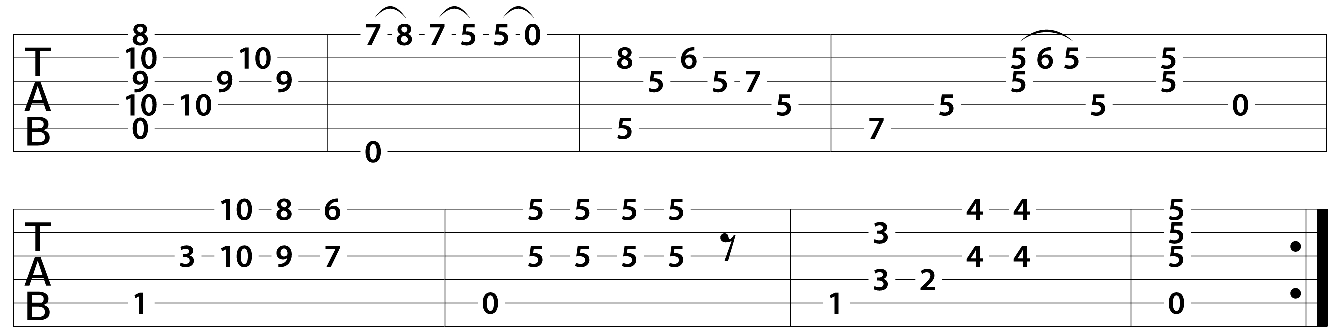
\includegraphics[width=365pt, height=100pt ]{res/darmodej.pdf}
\end{figure}
}
}


\toftagthis{vw}
\song{David a goliáš}{J. Ježek / V+W}{10pt}{0.99}{
\crdheight=2.3ex
\verse{1}{}\C{}Lidi na li\Am{}di jsou jako \F{}san\G[7]{}ě, \hskip 1em
\C{}člověk na člo\Am{}věka jako \F{}kat\G[7]{},\\
\C{}podívejte \A[7]{}se na ně, \Dm{}musíte \G[7]{}naří\C{}kat.\H[7]{}\\
\Em{}Obr do pidimužíka \A{}myd\H[7]{}lí, \hskip 0.8em \Em{}domnívaje se, že vyhra\A{}je,\H[7]{}\\
\G{}klidně \Em{}seďme \Am{}na žid\D[7]{}li, \hskip 0.8em \G{}čtěme bibli, \G[7]{}tam to všechno je.

\verse{2}{}\C{}Samuelo\Am{}va kniha nám \Dm[7]{}poví - \G[7]{}dá,\\
\C{}jak na žida \Am{}přišla veli\Dm[7]{}ká bí - \G[7]{}da,\\
\C{}jak ti bídní \Am{}Filištíni \F{}válku vést ne\Fm{}byli líní,\\
\C{}až potkali \Ab[7]{}Davi\G[7]{}da. 

\verse{3}{}\C{}David šel do \Am{}války volky, \Dm[7]{}nevol - \G[7]{}ky,\\
\C{}z velké dálky \Am{}nesl bratrům \Dm[7]{}homol - \G[7]{}ky,\\
\C{}v pochodu se \Am{}cvičil v hodu, \F{}dal si pro strý\Fm{}čka Příhodu\\
\C{}tři šutry do \G[7]{}tobol\C{}ky.

\verse{*}{}\uv{Hej, \Ab{}hej, kam se \C{}valej, vždyť jsou \D[7]{}malej!}\\
Takhle \G[7]{}Goliáš ho \E[7]{}provokuje,  \Dm[7]{}David slušně \G[7]{}salutuje.

\verse{4}{}\C{}Když mu \Am{}ale obr plivnul \Dm[7]{}do očí,\G[7]{}\\
\C{}David se o\Am{}točí, prakem \Dm[7]{}zato - \G[7]{}čí,\\
\C{}když začínáš, \Am{}no tak tu máš, \F{}byl jsi velkej \Fm{}já měl kuráž\\
\C{}a jakej byl \D[7]{}Go - \G[7]{}li - \C{}áš!

~\\
\hskip 5em \emph{(pokračování dle verze z roku 1952)}\\
\leftskip 45pt
\rec{Vcelku, to co jsme dnes slyšeli, to není nic nového,\\
to je stará příhoda, ale zajímavá věc,\\
ono to má pokračování:}


\textbf{\textsf{Akordy jako ve 2.,3.,*.,4.}}\\
\verse{5}{}Jestli masy nebudou dost masívní\\
a zůstanou ještě pár let pasívní,\\
stanou se pak tyto masy asi už na věčné časy\\
radioaktívní.\\
\verse{6}{}Víte, co je zapotřebí nápadů,\\
jak se zbavit nukleárních odpadů,\\
víte-li, co zla natropí bez kontroly izotopy\\
tisíc let po dopadu.\\
\verse{*}{}Ba jó, my to víme a tvrdíme,\\
mějme hlavy v písku, jako pštrosi,\\
nejvejš nám to spálí šosy.\\
\verse{7}{}Jenže lidem nejde jenom o šosy,\\
ale o krk a o značný obnosy,\\
a proto by měly masy, říct své slovo všemi hlasy,\\
dřív než nás smrt pokosí!\\
}


\toftagthis{raduza}
\song{De nîmes}{Radůza}{50pt}{1}{
\verse{1}\Am{}Očima uhla \Dm{}jsem \Em{}a nebylo to stu\Am{}dem.\\
\Am{}Peřina pohla \Dm{}se, \hskip 1em \G{}nějak už \Am{}bude.\\
Lino je studený, ponožky a pak triko.\\
A kabát přes denim a nic a ticho.

\verse{*}Cette \Am{}chanson n’a jamais été chantée\\
\Dm{}comme il faut, c’est ça\\
Mais \G{}si tu veux, nous \Em{}tous les deux\\
pou\Am{}vons le faire, comme ça

La \Am{}tranquillité, c’est ce qu’on cherche on\\
\Dm{}dit: »Puisse-t-elle venir!«\\
On \G{}dit que tout est \Em{}dificile\\
mais, \Am{}qu’ est-ce que ça veut dire

\chorus{}\Am{}Zouvám si pár \Dm{}těžkejch bot,\\
jsi \G{}ve ves\Em{}míru můj \Am{}pevnej bod.\\
A sukně kasám, je blízko brod\\
a pryč je, co kdo zbod.

\verse{2}Jen hlesnu od dveří:
\uv{Víš, nelhala jsem dosud.\\
A jestli nevěříš,
zkus špičku nosu.}\\
Okna jsou zamžený,
nádobí škopek plnej,\\
mám hrdlo stažený,
hajej a nynej.\\
\verse{*}Cette chanson \dots\\
\chorus{}Zouvám si pár těžkejch bot \dots 

\verse{3}Očima uhla jsem
a nebylo to studem.\\
Poznal jsi po hlase
jak mi teď bude.\\
Lino je studený,
pod kafem stůl se kejvá.\\
Un souvenir de Nîmes,
tak už to bejvá.\\
\verse{*}Cette chanson \dots\\
\chorus{}Zouvám si pár těžkejch bot \dots\\
}


\toftagthis{olympic}
\song{Dej mi víc své lásky}{Olympic}{30pt}{0.89}{
\verse{1}{}\Em{}Vymyslel jsem spoustu nápadů, a\G{}úú\\
co \Em{}podporujou hloupou nála\D{}du, a\H[7]{}úú,\\
\Em{}hodit klíče do kanálu, \A{}sjet po zadku \Am{}holou skálu,\\
\Em{}v noci chodit \H[7]{}strašit do hra\Em{}du.

\verse{2}{}Dám si dvoje housle pod bradu, aúú,\\
v bíle plachtě chodím pozadu, aúú,\\
úplně melancholicky, s citem pro věc, jako vždycky,\\
vyrábím tu hradní záhadu, a\D[7]{}úú.

\vskip -1ex
\chorus{} \G{}Má drahá, dej mi víc, \H[7]{}má drahá, dej mi víc,\\
\Em{}má drahá, \C{}dej mi víc své \G{}lásky, a\D[7]{}úú.\\
\G{}Já nechci skoro nic, \H[7]{}já nechci skoro nic,\\
\Em{}já chci jen \C{}pohladit tvé \G{}vlásky, a\H[7]{}úú!

\verse{3}{}Nejlepší z těch divnejch nápadů, aúú,\\
mi dokonale zvednul náladu, aúú,\\
natrhám ti sedmikrásky, tebe celou s tvými vlásky\\
zamknu si na sedm západů, aúú.\\
\textbf{R:}

\verse{4. = 3}{}\ldots{}+ aúú, aúú, aúú, aúú. 
}

\toftagthis{nohavica}
\song{Divoké koně}{Jaromír Nohavica}{15pt}{1}{
\capo{5}
\verse{1}\revrpt{} \Em{}Já viděl divoké koně, \G{}běželi \Am{}soumra\Em{}kem, \rpt{}\\
\Am{}vzduch \Em{}těžký \Am{}byl a divně \Em{}voněl\Ds[dim]{} \hskip 1em tabá\C{}kem,\\
\Am{}vzduch \Em{}těžký \Am{}byl a divně \Em{}voněl \H[7]{}tabá\Em{}kem.

\vskip -1ex
\verse{2}\revrpt{} Běželi, běželi, bez uzdy a sedla, krajinou řek a hor, \rpt{}\\
\revrpt{} sper to čert, jaká touha je to vedla za obzor. \rpt{}

\vskip -2ex
\verse{3}\revrpt{} Snad vesmír nad vesmírem, snad lístek na věčnost, \rpt{}\\
\revrpt{} naše touho ještě neumírej, sil máme dost. \rpt{}

\vskip -2ex
\verse{4}\revrpt{} V nozdrách sládne zápach klisen na břehu jezera, \rpt{}\\
\revrpt{} milování je divoká píseň večera. \rpt{}

\vskip -2ex
\verse{5}\revrpt{} Stébla trávy sklání hlavu, staví se do šiku, \rpt{}\\
\revrpt{} král s dvořany přijíždí na popravu zbojníků. \rpt{}

\vskip -2ex
\verse{6}\revrpt{} \scalebox{0.97}[1]{\textls[-40]{Chtěl bych jak divoký kůň běžet běžet, nemyslet na návrat,\,}}\rpt{}\\
\revrpt{} s koňskými handlíři vyrazit dveře, to bych rád. \rpt{}

\vskip -1ex
Já viděl divoké koně!\\
\vskip 12pt
\begin{figure}[h!]
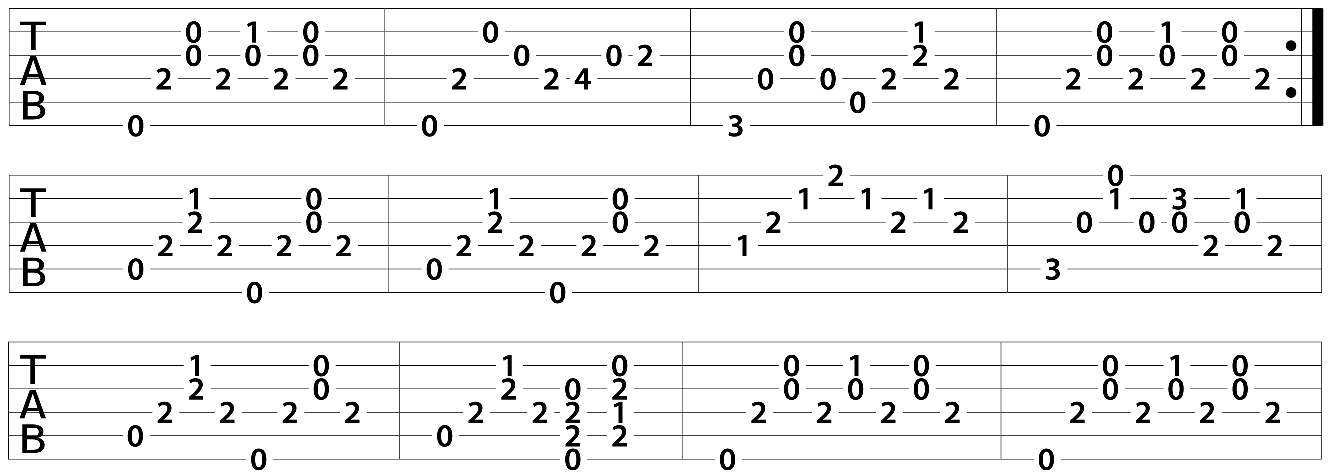
\includegraphics[width=365pt ]{res/divoke.pdf}
\end{figure}
\vskip -40pt
}


\toftagthis{hapka}
\song{Dívám se, dívám}{Petr Hapka / Michal Horáček}{12pt}{1}{
\verse{1}\D{}Dívám se, dívám a ty \A{}spíš, matně se leskne malý \G{}kříž.\\
Stoupá a klesá tvoje hruď\\
a já si říkám: \uv{Bůh jen \D{}suď, Bůh jen \A{}suď.}

\verse{2}Zdali, až jednou blýskne se a vítr liják přinese,\\
vezmeš mě k teplu pod svůj plášť.\\
Jestli to pro mě uděláš?

\verse{*}\D{}Když budu sedět nehnu\A{}tě a zase \D[maj]{}znovu zklamu \E{}tě\\
svým dojmem, že jsem na pouš\D{}ti\\
a že mě štěstí opouš\A{}tí,\hskip 1em \E{}

\verse{3}\D{}Zeptáš se: \uv{Kam jsi oči \A{}dal? Tvá šťastná hvězda svítí \G{}dál!\\
Jdi za ní, já tu držím stráž\ldots}\\
\chorus{}\revrpt{} \D{}Tak se \G[maj]{}ptám, jestli to \A{}uděláš, \rpt{}\\
pro mě \D{}uděláš.

\verse{4}\F{}Co když se těžce zadlu\C{}žím? I ten kříž prodáš? Co já \Bb{}vím.\\
Když mě mé masky unaví,\\
stáhneš mě k sobě do trá\F{}vy, do trá\C{}vy.

\verse{5}\uv{A klidně řekneš hroznou lež: Na svoje léta hezkej seš.\\
Před sebou ještě všechno máš\ldots}\\
Jestli to pro mě uděláš?

\verse{*}\F{}Co když mě zapřou přáte\C{}lé a budu s \F[maj]{}cejchem na \G{}čele\\
podroben strašné žalo\F{}bě? Vzkážeš mi: \uv{Stojím při to\C{}bě!\\
Jen při to\G{}bě.

\verse{6}Jediná vždycky budu stát i když ti celý svět dá mat.\\
Věřím ti všecko. Braň se, snaž\ldots}\\
\chorus{}\revrpt{} \F{}Jen se \Bb[maj]{}ptám, zda to \C{}uděláš. \rpt{}\\
Pro mě udě\F{}láš.

\verse{7}\D{}Stou\CHORD{\ldots}{}pá a klesá tvoje hruď, tak spolehlivě jako rtuť,\\
na teploměru našich dní,\\
ráno svět zuby vycení, vycení.

\verse{8}A mně se mnohé nezdaří, ale tvé prsty po tváři\\
mi zvolna přejdou, každý zvlášť.\\
\chorus{}Vím, že to pro mě uděláš.\\
Já vím, že to pro mě uděláš.\\
Všechno uděláš.
}


\toftagthis{brichta}
\song{\textls[-10]{Dívka s perlami ve vlasech}}{Aleš Brichta}{60pt}{0.9}{
\setlength{\parskip}{1ex} % vertical space between paragraphs
\verse{1}{}\Em{}Zas mě tu \D{}máš, ně\Am{}jak se \Em{}mračíš,\\
vybledlej smích už ve dveřích.\\
S čelenkou perel svatozář ztrácíš,\\
kolik se platí za vláčnej hřích.

\chorusAlt{R1:}{-29pt}No tak lás\G{}ko, co \D{}chceš mi říct,\\
\Am{}máš už perly, mož\Em{}ná i víc,\\
lásko, na co se ptáš, svíčku zhasínáš.\\
Nemám, lásko, co bych ti dal,\\
chtělas všechno, nebyl jsem král,\\
lásko, na co se ptáš, perly ve vlasech máš.

\verse{2}{}Tvý horky rty, víc radši ne,\\
nejsou už mý, nejsi má Cher.\\
Něco snad chápu, to ne, to ne,\\
bolí to, hořím, jak černej thér.

\chorusAlt{R2:}{-30pt}No tak lásko, kdo mi tě vzal,\\
komus dala, tělo i duši,\\
lásko, na co je pláč, když to skončit má.\\
Vždyť už, lásko, svý perly máš,\\
tak proč padaj', měněj se v slzy,\\
lásko, na co je pláč, perly ve vlasech máš.

\verse{3}{}Chtěla jsi víc pro svoje touhy,\\
já, chudej princ, mám jen, co mám.\\
Co vlastně zbývá, jen slzy pouhý,\\
ze svatebních zvonů, z nebeskejch bran.\\
\textbf{R2: + R1:}
}


\toftagthis{chinaski}
\song{Dlouhej kouř}{Chinaski}{25pt}{1}{
\verse{1}\D{}Když budeš hodná, naučím tě \C{}číst, naučím tě \G{}číst\\
mezi řádky.\\
To pokušení znáš, tak zapomeň cestu zpátky.\\
Hmm\ldots cestu zpátky.\\
Naše noc je mladá, vane jižní vítr,\\
papírový křídla vzduchem víří.\\
Řekni, co bys ráda, než nám ráno plány zkříží.

\verse{*}Půjdem nekonečně dlouhou sametově černou tmou.\\
Půjdem nekonečně dlouhou sametově černou\ldots

\chorus{}Vam pam tyda pam, dám si ruce do kapes.\\
vam pam tyda pam, dlouhej kouř a pohoda jazz.\\
vam pam tyda pam, neštěkne po mě ani pes.\\
padám a nevím kam, nečekej, že ti zavolám.

\verse{2}Když budeš hodná, moje hodná holka,\\
ukážu ti všechny svoje tajný skrýše.\\
Poletíme vejš, chvíli budem řvát, chvíli budem tiše.\\
Úplně tiše\ldots\\
Vezmu si tě celou, budem se mít rádi\\
a když ne, tak se ti něco zdálo.\\
A když budem chtít, šlápnem na zmizík,\\
všechno bude málo.

\verse{*}Půjdem nekonečně dlouhou\ldots + \textbf{R:}\\
}


\toftagthis{klus}
\song{Do nebe}{Tomáš Klus}{20pt}{1}{
\transposeFiveDown 
\verse{1}Haló, \C{}pane,\G{} vy s \Am{}výhledem na celej svět,\F{}\\
co se \C{}stane,\G{} když \Am{}neumím dát odpo\F{}věď?\\
Snad se \C{}nezlobíte,\G{} snad mi to \Am{}odpustíte,\F{}\\
vždyť \F{}víte, \F{}že chci\ldots

\chorus{}\revrpt{} Do nebe, do nebe, do nebe, do nebe, do nebe,\\
do nebe, do nebe, do nebe, do nebe,\\
do nebe, do nebe, do nebe, do nebe, do nebezpečna. \rpt{}

\verse{2}Haló, pane, nad střechami paneláků,\\
až déšť ustane, až uschnou křídla ptáků,\\
budu relativně štastný, budu žádaný a krásný,\\
budu obdivován v očích půvabných dam, ale sám\\
půjdu\ldots\\
\textbf{R:}

\verse{3}Haló, pane, vy s šedivými vousy,\\
jak poznat nepoznané, jak štěstí nevytrousit,\\ 
jak se nadechnout a zůstat živ a zdráv\\
a jestli jít či plout, to bych taky věděl rád,\\
vždyť chci\ldots\\
\textbf{R:}\\
}

\toftagthis{chinaski}
\song{Dobrák od kosti}{Chinaski}{40pt}{0.95}{
\verse{1}{}\C{}Má milá, \G{}jak ti je, tak \F{}jak ti je?\F{}\\
\C{}Jsem ten, kdo \G{}jednou tvý \F{}tělo zakryje.\Bb{} \hskip 1em \emph{\normalsize \textbf{Fine}}\\
Jsem ten, kdo tě jednou oddělá,\\
potkalas zkrátka kohos neměla.

\verse{2}{}Jsi budoucí krev v mojí posteli.\\
Jsem ten, kdo tě jednou jistojistě zastřelí,\\
jsem ten, kdo ty tvoje krásný oči jednou zatlačí.\\
Jsi moje všechno a mně to nestačí.\\
\chorus{}Je to \C{}vážně silná káva, \G{}pláč a nebo vztek,\\
\F{}nic už s tím nenadě\F{}láš.\\
Nech mě jenom hádat, jak jsi hebká na dotek,\\
krásná a nedospělá. 

\verse{3}{}Víš,všechno má aspoň malý kaz,\\
jsem ten, kdo ti jednou zlomí vaz.\\
Má milá, vždyť mě znáš, jsem dobrák od kosti\\
a ty jsi ta, co mi to jednou všechno odpustí. 

\verse{*}{}\revrpt{} Sejde z očí, sejde z mysli,\\
jenom blázen věří na nesmysly,\\
láska je čaroděj a ticho prý léčí,\\
ale zákon hovoří jasnou řečí. \rpt{}\\
\textbf{R:, R: (kluci) + *. (holky)\\ 1. al Fine }
}


\toftagthis{nohavica}
\song{Dokud se zpívá}{Jaromír Nohavica}{22pt}{1}{
\verse{1}{}\C{}Z Těšína \Em{}vyjíždí \Dm[7]{}vlaky co \F{}čtvrthodi\C{}nu,\Em{} \hskip 2.1em  \Dm[7]{} \hskip 2.8em  \G[7]{}\\
\C{}včera jsem \Em{}nespal a \Dm[7]{}ani dnes \F{}nespoči\C{}nu,\Em{} \hskip 2.1em  \D[7]{} \hskip 2.8em  \G[7]{}\\
\F{}svatý \G{}Medard, můj \C{}patron, ťuká \Am{}si na če\G{}lo, \G{}\\
ale \F{}dokud se \G{}zpívá, \F{}ještě se \G{}neumře\C{}lo. \Em{} \hskip 2.1em  \Dm[7]{} \hskip 2.8em  \G[7]{}

\verse{2}{}Ve stánku koupím si housku a slané tyčky,\\
srdce mám pro lásku a hlavu pro písničky,\\
ze školy dobře vím, co by se dělat mělo,\\
ale dokud se zpívá, ještě se neumřelo. 

\verse{3}{}Do alba jízdenek lepím si další jednu,\\
vyjel jsem před chvílí, konec je v nedohlednu,\\
za oknem míhá se život jak leporelo,\\
ale dokud se zpívá, ještě se neumřelo. 

\verse{4}{}Stokrát jsem prohloupil a stokrát platil draze,\\
houpe to, houpe to na housenkové dráze,\\
i kdyby supi se slítali na mé tělo,\\
tak dokud se zpívá, ještě se neumřelo. 

\verse{5}{}Z Těšína vyjíždí vlaky až na kraj světa,\\
zvedl jsem telefon a ptám se: \uv{Lidi, jste tam?}\\
A z veliké dálky do uší mi zaznělo,\\
\revrpt{} že dokud se zpívá, ještě se neumřelo. \rpt{}\\
}


\toftagthis{kabat}
\song{Ďábel a syn}{Kabát}{25pt}{1}{
\verse{1}{}\Dm{}Sedím a koukám, jak \C{}zvrácenej podzim\\
\Am{}stromům svlíká jejich \G{}šat,\\
poslouchám ptáky a jenom tak kouřím,\\
malinko chce se mi spát.\\
Padá mi hlava, pak cejtím, jak někdo\\
lehce mě za ruku vzal,\\
blázen či voják, jak maškara divná tam \Am{}stál\ldots{}\\
já pozval ho \Dm{}dál 

\verse{2}{}Měl špinavej kabát a v ruce flétnu,\\
oči jak z mrtvejch by vstal,\\
na botách bahno snad celýho světa,\\
tuhletu píseň mi hrál.\\
Tu píseň, co zpívám, a vůbec vám nevím,\\
kde na ni akordy vzal,\\
jak jsem tam seděl a koukal a kouřil, to já\ldots{}\\
teprv ji psal.  

\verse{3}{}Povídá: \uv{Hochu, vracím se z flámu,\\
hráli jsme karty se zdá,\\
partii pokera o budoucí vládu,\\
dík bohu vyhrál jsem já.\\
Já měl z pekla štěstí a nebo pár trumfů\\
v rukávu -- podvod, já vím,\\
chcete mě soudit, tak dejte mě na kříž, jsem váš\ldots{}\\
ďábel a syn.}  

\verse{4}{}Pak pomalu mluvil a ničil mě silou,\\
co od věků v sobě už má,\\
drtil mě pravdou a pouštěl mi žilou,\\
na závěr jen povídá:\\
\uv{Bůh stvořil lásku a žal, taky bolest\\
a já jenom ubohej chtíč,\\
fandím vám lidem, nevím proč nemáš mě rád\ldots{}}\\
já poslal ho pryč.  

\verse{5}{}Sedím a koukám, jak zvrácenej podzim\\
stromům svlíká jejich šat,\\
přemejším o tom, co s náma bude\\
a malinko chce se mi spát.\\
Padá mi hlava, pak cejtim, jak někdo\\
lehce mě za ruku vzal,\\
blázen či voják, jak maškara divná tam stál\ldots{}\\
tak pozvem ho dál.\\
}


\toftagthis{matuska}
\song{Eldorádo}{Waldemar Matuška}{30pt}{1}{
\verse{1}{}\Am{}V dálných \G{}dálkách zámo\Am{}ří ční prý \G{}zlaté poho\Am{}ří,\\
\Am{}přícho\C{}zího pohos\D{}tí \hskip 0.2em \Dm{}nádhe\C{}rou a hojno\G{}stí. \E[7]{}

\verse{2}{}Dík těm svůdným pověstím zástupy šly za štěstím,\\
chátra i ti bohatí s vírou, že se vyplatí\ldots{}

\chorus{}\Am{}Jít a hledat Eldo\G{}rádo zbave\C{}né vší \D{}bídy člově\G{}čí,\E[7]{}\\
\Am{}jít a hledat Eldo\G{}rádo, kde je \C{}láska, \D{}mír a bezpe\Em{}čí. 

\verse{3}{}\Hm{}Báchor\A{}ce té uvě\Hm{}ří  dávno \A{}už jen někte\Hm{}ří,\\
\Hm{}spíš než \D{}zlatonosný \E{}štít \Em{}nám dnes \D{}rozum káže \A{}jít \Fs[7]{}\ldots 

\chorus{}\Hm{}Jít a hledat Eldo\A{}rádo zbave\D{}né vší \E{}bídy člově\A{}čí,\Fs[7]{}\\
\Hm{}jít a hledat Eldo\A{}rádo, kde je \D{}láska, \E{}mír a bezpe\Fsm{}čí.\\
}


\toftagthis{sverakuhlir}
\song{Elektrický valčík}{Z. Svěrák / J. Uhlíř}{25pt}{0.89}{
\vskip -5pt
\capo{4}
\vskip 5pt
\verse{1}{}\Am{}Jednoho letního večera na návsi pod starou \E[7]{}lípou\\
hostinský Antonín Kučera vyvalil soudeček s \Am{}pípou.\\
Neby\F{}lo to posvícení, neby\Am{}la to neděle,\\
v naší \F{}obci mezi kopci plni\E[7]{}ly se korbele.

\vskip -2ex
\chorus{}\A{}Byl to ten slavný den, kdy k nám byl zaveden\noexport{\\} \E[7]{}elek\E[dim]{}trický \E[7]{}proud,\\
\E[7]{}byl to ten slavný den, kdy k nám byl zaveden\noexport{\\} \A{}elek\A[dim]{}trický \A{}proud,\\
\A[7]{}střída\D{}vý, \E{}stříd\Csm{}avý, \hskip 0.8em \Fsm{}silný \hskip 0.2em \Hm{}elekt\E[7]{}rický \A{}proud,\\
\A[7]{}střída\D{}vý, \E{}stříd\Csm{}avý, \hskip 0.8em \Fsm{}zkrátka \Hm{}elekt\E[7]{}rický \Am{}proud.

\rec{\textls[-18]{A nyní, kdo tu všechno byl:\\
Okresní a krajský inspektor, hasičský a recitační sbor,\\
poblíže obecní váhy tříčlenná delegace z Prahy,\\
zástupci nedaleké posádky pod vedením poručíka Vosátky,\\
početná družina montérů, jeden z nich pomýšlel na dceru\\
sedláka Krušiny, dále krojované družiny,\\
alegorické vozy, italský zmrzlinář Antonio Cosi\\
na motocyklu Indián a svatý Jan, z kamene vytesán.}}\\
\textbf{R:}

\linespread{1} \selectfont
\verse{2}{}\textls[-18]{Na stránkách obecní kroniky ozdobným písmem je psáno,}\\
tento den pro zdejší rolníky znamenal po noci ráno,\\
budeme žít jako v Praze, všude samé vedení,\\
jedna fáze, druhá fáze, třetí pěkně vedle ní.\\
\textbf{R:}

\rec{\textls[-25]{Z projevu inženýra Maliny, zástupce Elektrických podniků:\\
\uv{Vážení občané, vzácní hosté, s elektřinou je to prosté:\\
od pantáty vedou dráty do žárovky nade vraty,\\
odtud proud se přelévá do stodoly, do chléva,\\
při krátkém spojení dvou drátů\\dochází k takzvanému zkratu,\\
kdo má pojistky námi předepsané,\\tomu se při zkratu nic nestane,\\
kdo si tam nastrká hřebíky, vyhoří a začne od píky.\\
Do každé rodiny elektrické hodiny!}}}\\
\textbf{R:}

\noexport{
~\\
\hskip -20pt \textbf{Akordy:}\\
\hskip -15pt \begin{minipage}[t]{\textwidth} \chord{t}{o,p1,p2,o,p2,o}{Edim} \end{minipage}
\hskip 0pt\begin{minipage}[t]{\textwidth}\chord{t}{x,o,p1,p2,p1,p2}{Adim} \end{minipage}
}
}


\toftagthis{vw}
\song{Ezop a brabenec}{J.Ježek / V+W}{20pt}{1}{
\verse{1}{}\C{}Jednou \Em{}z lesa \Am{}domů se \Am[7]{}nesa \hskip 0.5em \F{}mou\G[7]{}drý \C{}Ezop\G[7]{}\\
\C{}potkal \Em{}brabce, \Am{}který bra\Am[7]{}bence \F{}má\G[7]{}lem \A[7]{}sezob.\\
\Dm{}Brabenec se \E{}chechtá, \Dm{}Ezop se ho \D[7]{}hned \G[7]{}ptá,\\
\C{}čemu \Em{}že se \Am{}na trávě \Am[7]{}v lese \F{}prá\G{}vě \Dm{}řeh - \G[7]{}tá.

\verse{2}{}\uv{\C{}Já,} povídá \G[7]{}brabenec, \uv{se taky \C{}rád\Bb{} hlasitě \A[7]{}chechtám,\\
chech\D[7]{}tám, když pupe\Ab[7]{}nec kyse\G[7]{}linou lep\C{}tám\D[7]{}. \hskip 1.2em \Dm[7]{} \hskip 2.8em \G[7]{}\\
\C{}Vím,} totiž ten \G[7]{}brabenec, \uv{mraveneč\C{}ník\Bb{} že se mě \A[7]{}neptá,\\
ne\D[7]{}ptá, pozře mě \Ab[7]{}ať se chech\G[7]{}tám nechech\C{}tám\Dm{}.} \hskip 1.3em \G[7]{} \hskip 1.6em \C{}

\verse{3}{} \Ab{}Kampak by to \Eb[7]{}došlo třeba s \Ab{}pouhou ponra\Eb[7]{}vou,\\
\G{}kdyby měla \D[7]{}plakat, že je \Dm{}ptačí potra\G[7]{}vou.\\
~\\
\verse{4}{}\C{}Ty, ač nejsi \G[7]{}brabenec, se taky \C{}rád\Bb{} hlasitě \A[7]{}chechtej,\\
chech\D[7]{}tej a na svou \Ab[7]{}bídu si \G[7]{}nezarep\C{}tej.\\
}


\toftagthis{anglicke, sunrise}
\song{Fairytale Gone Bad}{Sunrise Avenue}{30pt}{1}{
\bigskip

\Hm[11]{} \hskip 3.2em  \G[add9]{} \hskip 3.4em \A[sus4]{} \hskip 3.2em \Em[7add11]{}\\
\verse{1}This is the \Hm{}end, you \G{}know,\\
\D{}lady, the plans we had went all wrong,\\
\A{}we ain't nothing but \E[/G$\sharp$]{}fight and shout and \Hm{}tears.

We got to a point I can't stand,\\
I've had it to the limit, I can't be your man,\\
I ain't more than a minute away from walking.

\verse{*}\G[add9]{}We can't \D[5]{}cry the \A[add9]{}pain \hskip 1em a\G[add9]{}way,\\
we can't \D[5]{}find a \A[add9]{}need to \G[add9]{}stay,\\
I slowly\D[5]{} real\A[add9]{}ize there's \G[add9]{}nothing on our \A[add9]{}side.

\chorus{}\Hm[11]{}Out of my life, out of my mi\G[add9]{}nd,\\
out of the tears, we can't de\A[add9]{}ny,\\
we need to \D[sus2/F$\sharp$]swallow all our \G[add9]{}pride\\
and leave this mess behi\A[add9]{}nd.

Out of my head, out of my bed,\\
out of the dreams we had, they're bad,\\
tell them it's me who made you sad,\\
tell them the fairy\Fs[/A$\sharp$]{}tale gone bad.

\verse{2}Another night and I bleed,\\
they all make mistakes and so did we,\\
but we did something we can never turn back right.

Find a new one to fool,\\
leave and don't look back, I won't follow,\\
we have nothing left, it's the end of our time.

\verse{*}We can't cry the pain away,\\
we can't find a need to stay,\\
there's no more rabbits in my hat to make things right.\\
\textbf{R: $(2\times)$}\\

\Hm[11]{} \hskip 3.2em \G[add9]{} \hskip 3.4em \A[sus4]{}Tell them the f\Em[7add11]{}airytale gone bad.\\
\Hm[11]{} \hskip 3.2em \G[add9]{} \hskip 3.4em \A[sus4]{}Tell them the f\Em[7add11]{}airytale gone bad.\\

\Hm[11]{} \hskip 3.2em  \G[add9]{} \hskip 3.4em \A[sus4]{} \hskip 3.2em \Em[9]{}\\
}


\toftagthis{anglicke}
\song{Falling Slowly}{Glen Hansard \& Markéta Irglová}{20pt}{1}{
\verse{1}
\C{}I don't know you, \F{}but I want you\\
\C{}all the more for \F{}that.\\
Words fall through me and always fool me\\
and I can't react.

\verse{*}\Am{}Games that \G{}never a\F{}mount
to \G{}more than they \Am{}meant,\\
will \G{}play themselves \F{}out.

\chorus{}\C{}Take this sinking \F{}boat and point it \Am{}home,\\
we've still got \F{}time.\\
Raise your hopeful voice, you had the choice,\\
you've made it now.

\verse{2}Falling slowly, eyes that know me\\
and I can't go back,\\
Moods that take me and erase me\\
and I'll paint it black.

\verse{*}You have suffered enough and warred with yourself,\\
it's time that you won.\\
\textbf{R:}\\
Falling slowly, sing your melody,\\
I'll sing along.\\
}


\toftagthis{ceskekapely}
\song{Fousy}{Poletíme?}{60pt}{1}{
\verse{1}Když se \C{}zeptáte, proč nosím plnofous,\\
jestli mě třeba pes do brady \D{}kous,\\
jestli \F{}mám tam vyráž\C{}ku,\\
a nebo \Dm{}něco schová\C{}vám,\\
tak vám \D{}jak odpověď tohle zazpí\G{}vám:

\verse{2}Mít fous mi přijde normální,\\
nemít fous – nenormální,\\
kašlu na trendy, takhle jsem se narodil,\\
bůh mě stvořil, abych takhle chodil.

\verse{3}Za fousy mě z mámy vytáhli,\\
i ve škole mně fousy nechali,\\
první holku jsem sbalil fousem\\
ostatní už na fous čekaly.

\chorus{}Fousy, fousy, fousy, fousy, fous\ldots

\verse{4}Podle fousů se lidi poznají,\\
fousy fousům fousy mávají,\\
člověk bez fousů je jako kocour bez fousů,\\
jako kaktus bez fousů, jako Mikuláš bez fousů.\\
\textbf{R:}

\verse{5}Jednou mně mé fousy zešednou,\\
budou se fousit chůzi šoulavou,\\
a pak buďte si jistí za co mě spustí,\\
v díru v zemi vykopanou.

\verse{6}V nebi všichni svatí fousatí,\\
mě mezi fousaté posadí,\\
a budem pak fousy zdravit ty, co si\\
užívají věčné holení na věčnosti.\\
\textbf{R: (2$\times$)}
}


\toftagthis{brontosauri}
\song{Franky dlouhán}{Brontosauři}{40pt}{0.87}{
\verse{1}Kolik je \C{}smutného, když \F{}mraky černé \C{}jdou\\
lidem nad hla\G[7]{}vou, \F{}smutnou dála\C{}vou.\\
Já slyšel příběh, který velkou pravdu měl,\\
za čas odletěl, každý zapomněl.

\vskip -1ex
\chorus{}\C{}Měl kapsu \G[7]{}prázdnou Franky Dlouhán,\\
po státech \F{}toulal se jen \C{}sám\\ 
a že byl \F{}veselej, tak \C{}každej měl ho \G[7]{}rád.\\
Tam ruce k \F{}dílu mlčky přiloží a \C{}zase jede \Am{}dál\\
a \F{}každej, kdo s ním \G[7]{}chvilku byl,\\
tak \F{}dlouho \G[7]{}se pak \C{}smál.

\verse{2}Tam, kde byl pláč, tam Franky hezkou píseň měl,\\
slzy neměl rád, chtěl se jenom smát.\\
A když pak večer ranče tiše usínaj',\\
Frankův zpěv jde dál, nocí s písní dál.\\
\textbf{R:}

\verse{3}Tak Frankyho vám jednou našli, přestal žít,\\
jeho srdce spí, tiše smutně spí.\\
Bůh ví jak, za co tenhle smíšek konec měl,\\
farář píseň pěl, umíraček zněl.\\
\textbf{R:}\\
}


\toftagthis{buty}
\song{František}{Buty}{50pt}{0.95}{
\verse{1}{}\G{}Na hladinu rybníka svítí sluníč\C{}ko\\
\Em{}a kolem stojí v hustém kruhu \G{}topoly,\\
\Am{}které tam zasadil jeden hodný \Hm{}člověk,\\
\Am{}jmenoval se František \D{}Dobrota.

\vskip -2ex
\verse{2}{}František Dobrota, rodák z blízké vesnice,\\
měl hodně dětí a jednu starou babičku,\\
která, když umírala, tak mu řekla: \uv{Františku,\\
teď dobře poslouchej, co máš všechno udělat.}

\vskip -2ex
\chorus{}\revrpt{} \C{}Balabambam, balabambam\C{} \hskip 1em \D{} \rpt{} $^{3\times}$\\
a \Am{}kolem rybníka nahusto nasázet \D{}topoly. 

\verse{3}{}František udělal všechno, co mu řekla,\\
a po snídani poslal děti do školy.\\
Žebřiňák s nářadím dotáhl od chalupy k rybníku,\\
vykopal díry a zasadil topoly.

\vskip -2ex
\verse{4}{}Od té doby vítr na hladinu nefouká,\\
takže je klidná jako velké zrcadlo,\\
sluníčko tam svítí vždycky rádo,\\
protože tam vidí Františkovu babičku.\\
\textbf{R:}\\
\noexport{
\vskip 5pt
\leftskip 0pt
\textbf{\emph{\large Flétna:}}
\setlength\parindent{0pt}
\begin{minipage}[m]{\textwidth}
\begin{music}
\input musixext
\instrumentnumber{1}
\generalsignature1
\nobarnumbers
\setsize 1\smallvalue
\hsize 247pt
\generalmeter\meterC
\nostartrule
\startpiece
\notes\hsk\ibl0h{0}\qb0n\nbbl0\qb0l\tbl0\qb0n\ibl1h0\qb1l\tbl1\qb1j\enotes
\notes\qlp{g} \hsk \ca{f}\enotes\bar
\notes \ibl2h0\qb2g\qb2j\qb2l\tbl2\qb2n\ibl3h{0}\qb3m\nbbl3\qb3n\tbl3\qb3m\cl{l}\ds\enotes
\endpiece
\end{music}
\end{minipage} 
}
}


\toftagthis{ceskekapely}
\song{Gastrosexuál}{Wohnout}{30pt}{0.96}{
\capo{2}
\verse{1}\Em{}Můj doktor sebou \D{}sek' a \A{}málem to neu\Em{}stál.\\
Víš, já mu tehdy řek, že jsem gastrosexuál.\\
Ale jen, co se z lehu zved, přísně se zazubil.\\
\Em{}Blíž jsem si k němu \D{}sed a \A{}všechno mu vyklo\C{}pil.

\chorus{}Do \Am{}příboru se oša\D{}tím a nebude mi \Em{}zima,\C{}\\
\Am{}stříknu pivo na ru\D{}kávy a kolu do ga\Em{}tí, \hskip 1em \D{}\\
vzít si boty z kaviáru není volovina,\\
na \Am{}léto si pak uva\Hm{}řím šaty kopro\Em{}vý.

\verse{2}Doktor řek:\uv{No, pane Homola,
tím jste mě zaskočil.\\
Přemýšlím stále dokola, 
čím bych vás vyléčil.\\
S tou tváří vaší nevinnou 
já bych nemarodil.\\
Zkuste svůj úlet rozvinout,}
doktor mi poradil.\\
\chorus{} \dots{} šaty koprový a gu\D{}lášo\A{}vý fi\Em{}ží.\\
Noha\Em{}vičky z marci\D{}pánu s vanil\A{}kovou příchu\Em{}tí.\\
Šál mazaný brušetou z tymiánu\\
a knof\Em{}líky ze sa\D{}lámu kula\A{}ťoučký vykro\C{}jím.

Náj na nana nananáj \dots

\chorus{}Do příboru se ošatím \dots{}
}


\toftagthis{anglicke}
\song{Hallelujah}{Leonard Cohen / Jeff Buckley}{30pt}{0.89}{
\verse{1}{}I've \G{}heard there was a \Em{}secret chord,\\
that \G{}David played, and it \Em{}pleased the Lord,\\
but \C{}you don't really \D{}care for music, \G{}do you? \D{}\\
It \G[/H]{}goes like this, the \C{}fourth, the \D{}fifth,\\
the \Em{}minor fall, the \C{}major lift,\\
the \D{}baffled king \H[7]{}composing Halle\Em{}lujah!

\chorus{}Halle\C{}lujah, Halle\Em{}lujah, Halle\C{}lujah, Halle\G{}lu-uu\D{}uu-u\G{}jah! 

\verse{2}{}Your faith was strong, but you needed proof,\\
you saw her bathing on the roof,\\
her beauty and the moonlight overthrew you.\\
She tied you to a kitchen chair,\\
she broke your throne, and she cut your hair,\\
and from your lips she drew the Hallelujah!\\
\textbf{R:}

\optVerse{-35pt}{27pt}{20pt}{
\verse{3}You say I took the name in vain,\\
I don't even know the name,\\
but if I did, well really, what's it to you?\\
There's a blaze of light in every word,\\
it doesn't matter which you heard,\\
the holy or the broken Hallelujah!\\
\textbf{R:}
}
~\\
\verse{4}{}Baby, I've been here before,\\
I know this room, I've walked this floor,\\
I used to live alone before I knew you.\\
I've seen your flag on the marble arch,\\
but love is not a victory march,\\
it's a cold and it's a broken Hallelujah!\\
\textbf{R:}

\verse{5}{}There was a time you let me know,\\
what's really going on below,\\
but now you never show it to me, do you?\\
But I remember, when I moved in you,\\
and the holy dove was moving too,\\
and every breath we drew was Hallelujah!\\
\textbf{R:}

\verse{6}{}Maybe there's a God above,\\
but all I've ever learned from love\\
was how to shoot at someone who outdrew you.\\
But it's not a cry that you hear at night,\\
it's not somebody who's seen the light,\\
it's a cold and it's a broken Hallelujah!\\
\textbf{R:}

\optVerse{-35pt}{27pt}{20pt}{
\verse{7}{}I did my best, it wasn't much,\\
I couldn't feel, so I tried to touch,\\
I've told the truth, I didn't come to fool you.\\
And even though it all went wrong,\\
I'll stand before the Lord of Song\\
with nothing on my tongue but Hallelujah!\\
\textbf{R: $(2\times)$}
}
}


\toftagthis{anglicke}
\song{Help!}{The Beatles}{20pt}{0.89}{
\crdheight=2.3ex
\verse{*}{}\Hm{}Help! I need somebody, \G{}help! Not just anybody,\\
\E{}help! You know I need someone, \A[7]{}help!

\verse{1}{}\A{}When I was younger, so much \Csm{}younger than today,\\
\Fsm{}I never needed anybody's \D{}help in \G{}any \A{}way.\\
But now these days are gone I'm \Csm{}not so self assured,\\
\textls[-25]{\Fsm{}now I find I've changed my mind I've \D{}opened \G{}up the \A{}door.}

\chorus{}\Hm{}Help me if you can I'm feeling down\\
and I \G{}do appreciate you being 'round,\\
\E{}help me get my feet back on the ground,\\
won't you \A{}please, please help me?

\verse{2}{}And now my life has changed in oh so many ways,\\
my independence seems to vanish in the haze.\\
But every now and then I feel so insecure,\\
I know that I just need you like I've never done before.\\
\textbf{R:}

\verse{3}When I was younger\ldots\\
\textbf{R:} \ldots{} please, please help \Fsm{}me, help me, help \A[6]{}me, ooh\ldots{}\\
}


\toftagthis{anglicke}
\song{Hit the Road, Jack}{Ray Charles}{20pt}{1}{
\chorus{}Hit the \Am{}road, \Am[/G]{}Jack, and \F{}don't you come \E{}back\\
no more, no more, no more, no more.\\
Hit the road, Jack, and don't you come back no more.\\
\emph{(What you say?)}\\
Hit the road, Jack, and don't you come back\\
no more, no more, no more, no more.\\
Hit the road, Jack, and don't you come back no more.

\verse{1}Woah Woman, oh woman, don't treat me so mean,\\
You're the meanest old woman that I've ever seen.\\
I guess if you say so\\
I'd have to pack my things and go.\\
\textbf{R:}

\verse{2}Now baby, listen baby, don't ya treat me this-a way\\
Cause I'll be back on my feet some day.\\
Don't care if you do 'cause it's understood\\
you ain't got no money you just ain't no good.\\
Well, I guess if you say so\\
I'd have to pack my things and go.\\
\textbf{R:}\\
\revrpt{} \ldots{}don't you come back no more. \rpt{}\\

}



\toftagthis{nohavica}
\song{Hlídač krav}{Jaromír Nohavica}{40pt}{0.95}{
\verse{1}{}\D{}Když jsem byl malý, říkali mi naši:\\
\uv{Dobře se uč a jez chytrou kaši,\\
\G{}až jednou vyrosteš, \A{}budeš doktorem \D{}práv.}\\
Takový doktor sedí pěkně v suchu,\\
bere velký peníze a škrábe se v uchu,\\
já jim ale na to řek': \uv{Chci být hlídačem krav.}

\chorus{}Já chci mít čapku s bambulí nahoře,\\
jíst kaštany a mýt se v lavoře,\\
od rána po celý den zpívat si jen,\\
zpívat si: pam pam pam\ldots{} 

\verse{2}{}K vánocům mi kupovali hromady knih,\\
co jsem ale vědět chtěl, to nevyčet' jsem z nich,\\
nikde jsem se nedozvěděl, jak se hlídají krávy.\\
Ptal jsem se starších a ptal jsem se všech,\\
každý na mě hleděl jako na pytel blech,\\
každý se mě opatrně tázal na moje zdraví.\\
\textbf{R:}

\verse{3}{}Dnes už jsem starší a vím, co vím,\\
mnohé věci nemůžu a mnohé smím,\\
a když je mi velmi smutno, lehnu si do mokré trávy.\\
S nohama křížem a rukama za hlavou\\
koukám nahoru na oblohu modravou,\\
kde se mezi mraky honí moje strakaté krávy.\\
\textbf{R:}\\
}

\toftagthis{zalman}
\song{Ho ho Watanay}{Pavel Lohonka Žalman / indiánská}{50pt}{1}{
\vskip 8pt
\verse{1}\D{}Spinkej, můj maličký, \C{}máš v očích \D{}hvězdičky,\\
dám ti je \C{}do vlasů, tak \G{}usínej tak \D{}usínej.

\chorus{}\D{}Ho ho Watanay, \C{}ho ho \D{}Watanay,\\
ho ho \C{}Watanay, Ki\G{}okena, Ki\D{}okena.

\verse{2}Sladkou vůni nese ti noční motýl z perleti,\\
vánek ho kolíbá, už usíná, už usíná.\\
\textbf{R:}

\verse{3}V lukách to zavoní, rád jezdíš na koni,\\
má barvu havraní, jak uhání, jak uhání.\\
\textbf{R:}

\verse{4}V dlani motýl usíná, hvězdička už zhasíná,\\
vánek co ji k tobě nes', až do léta ti odlétá.\\
\textbf{R:}\\
}


\toftagthis{anglicke}
\song{Hollywood Hills}{Sunrise Avenue}{20pt}{1}{
\capo{4}
\vskip 2ex
\verse{1}Now this \G{}is not the time or the place for brokenh\D[sus4/F$\sharp$]{}earted,\\
cause this is the end of the \Em[7]{}rainbow,\\
where no one can be\C[add9]{} \hskip 1em too \hskip 1em \Em[7]{}sad. \hskip 1em \D[sus4/F$\sharp$]{}\\
No, I don't wanna leave but I must keep moving ahead,\\
cause my life belongs to the other side,\\
behind the great ocean's waves.

\chorus{}\G{} Bye, bye, Hollywood Hill\G[/H]{}s, I'm gonna\\
\D{} miss you, wherever I g\D[/F$\sharp$]{}o, I'm gonna\\
\Em[7]{} come back to \Em[7/H]{}walk these streets again,\\
\C[add9]{} bye, bye, Hollywood Hi\D{}lls for\G{}ever.

\verse{2}Thank you for the morning walks on the sweet sunset\\
and for the hot night moments,\\
for the fantasy in my bed.\\
\scalebox{0.95}[1]{I take a part of you with me now and you won't get it back}\\
and a part of me will stay here,\\
you can keep it forever, \Em{}dear. Woo\A[7sus4]{}aooooo...\C[add9]{}

\clearpage
\leftskip 40pt
\chorus{}Bye, bye, Hollywood Hills, I'm gonna\\
miss you, wherever I go, I'm gonna\\
come back to walk this streets again,\\
remember that we had fun together. 

Bye, bye, rodeo girls, I'm gonna\\
love you, wherever I go, I'm gonna\\
come back, so we can play together,\\
bye, bye Hollywood Hills forever. 

\verse{3}Long distance love doesn't work,\\
all the miles in between get in your head.\\
No, I don't wanna go, I don't wanna go.

\chorus{}Bye, bye, Hollywood Hills, I'm gonna\\
miss you, wherever I go, I'm gonna\\
come back to walk these streets again,\\
bye, bye\ldots

\chorus{}Bye, bye, Hollywood Hills, I'm gonna\\
miss you, wherever I go, I'm gonna\\
come back to walk these streets again,\\
remember that we had fun together.

Bye, bye, rodeo girls, I'm gonna\\
love you, wherever I go, I'm gonna\\
come back, so we can play together,\\
bye, bye, Hollywood Hills forever.

Hollywood Hills forever,\\
Hollywood Hills forever\\}


\toftagthis{schelinger}
\song{Holubí dům}{Jiří Schelinger}{60pt}{0.93}{
\crdheight=2.3ex
\verse{1}{}\Em{}Zpí - \D{}vám \C[maj7]{}ptákům a \Hm[7]{}zvlášť holu\Em{}bům,\\
stá\D{}val v \C[maj7]{}údolím \Hm[7]{}mém starý \Em{}dům. \emph{\normalsize \textbf{Fine}}\\
\G{}Ptá\D{}ků \G{}houf zalé\D{}tal ke kro\G{}vům,\\
\Em{}měl\ \ \D{}jsem \C[maj7]{}rád holu\Hm[7]{}bích křídel \Em{}šum.

\vskip -2ex
\verse{2}{}Vlídná dívka jim házela hrách,\\
mávání perutí víří prach.\\
Ptáci krouží a neznají strach,\\
měl jsem rád starý dům, jeho práh.

\vskip -2ex
\chorus{}Hledám \Am[7]{}dům holu\D{}bí, kdopak z \G{}vás cestu \Em{}ví?\\
Míval \Am[7]{}stáj roube\D{}nou, bílý \G{}štít.\\
Kde je \Am[7]{}dům holu\D{}bí a ta \G{}dívka kde \Em{}spí?\\
Vždyť to \Am[7]{}ví, že jsem \Hm{}chtěl pro ni \Em{}žít.

\verse{3}{}Sdílný déšť vypráví okapům,\\
bláhový, kdo hledá tenhle dům.\\
Odrůstáš chlapeckým střevícům,\\
měl jsem rád holubích křídel šum.

\vskip -2ex
\verse{4}{}Nabízej úplatou cokoli,\\
nepojíš cukrových homolí.\\
Můžeš mít třeba zrak sokolí,\\
nespatříš ztracené údolí.\\
\textbf{R: + 1. al Fine}\\
}


\toftagthis{anglicke}
\song{Hotel California}{Eagles}{15pt}{1}{
\capo{2}
\verse{1}
\Am{}On a dark desert highway,\E{} cool wind in my hair,\\
\G{}warm smell of colitas\D{} rising up through the air.\\
\F{}Up ahead in the distance,\C{} I saw a shimmering light\\
\Dm{}My head grew heavy and my sight grew dim,\\
\E{}I had to stop for the night.

\verse{2}
There she stood in the doorway,\\
I heard the mission bell,\\
and I was thinking to myself:\\
\uv{This could be heaven or this could be hell.}\\
Then she lit up a candle\\
and she showed me the way.\\
There were voices down the corridor,\\
I thought I heard them say:

\chorus
\F{}Welcome to the Hotel Cali\C{}fornia,\\
such a \E{}lovely place, such a \Am{}lovely face.\\
\F{}Plenty of room at the Hotel Cali\C{}fornia,\\
any \Dm{}time of year you can \E{}find it here.
\clearpage
\verse{3}
Her mind is Tiffany-twisted, she got a Mercedes Benz,\\
she got a lot of pretty, pretty boys that she calls friends.\\
How they dance in the courtyard, sweet summer sweat.\\
Some dance to remember, some dance to forget.

\verse{4}
So I called up the captain: \uv{Please bring me my wine}\\
\uv{We haven't had that spirit here since 1969.}\\
And still those voices are calling from far away,\\
wake you up in the middle of the night,\\
just to hear them say:\\
\textbf{R:}

\verse{5}
Mirrors on the ceiling,\\
the pink champagne on ice, (and she said,)\\
\uv{We are all just prisoners here, of our own device.}\\
And in the master's chambers\\
They gathered for the feast,\\
They stab it with their steely knives,\\
but they just can't kill the beast. 

\verse{6}
Last thing I remember, I was running for the door,\\
I had to find the passage back to the place I was before.\\
\uv{Relax,} said the night man,\\
\uv{we are programed to receive.\\
You can check out any time you like,\\
but you can never leave.}

\chorus{}Welcome to the Hotel California,\\
such a lovely place, such a lovely face.\\
They livin' it up at the Hotel California,\\
what a nice surprise, bring your alibis.
}



\toftagthis{anglicke}
\song{House of the Rising Sun}{The Animals}{45pt}{0.9}{
\verse{1}There \Am{}is \hskip 0.5em a \hskip 0.5em \C{}house in \D{}New Orleans,\F{}\\
they \Am{}call the \C{}Rising \E{}Sun.\\
And it's \Am{}been the \C{}ruin of \D{}many a poor boy\F{}\\
and \Am{}God, I \E{}know, I'm \Am{}one. \hskip 0.5em \E{}

\verse{2}My mother was a tailor,\\
she sewed my new blue jeans,\\
my father was a gamblin' man\\
down in New Orleans.

\verse{3}Now the only thing a gambler needs\\
is a suitcase and trunk\\
and the only time he's satisfied\\
is when he's on a drunk.

\verse{4}Oh, mother, tell your children\\
not to do what I have done.\\
Spend your lives in sin and misery\\
in the House of the Rising Sun

\verse{5} Well, I got one foot on the platform,\\
the other foot on the train.\\
I'm goin' back to New Orleans\\
to wear that ball and chain.

\verse{6}There is a house\dots
}

\toftagthis{ceskekapely}
\song{Hrobař}{Premier}{70pt}{0.92}{
\verse{1}{}V \G{}mládí jsem se učil hrobařem,\\
\Em{}jezdit s hlínou, jezdit s trakařem,\\
\C{}kopat hroby byl můj ide\D{}ál. 

\verse{2}{}Jezdit s hlínou, jezdit s vozíkem,\\
s černou rakví, bílým pomníkem,\\
toho bych se nikdy nenadál.

\verse{3}V mládí jsem se\dots

\verse{4}Jezdit s hlínou\dots

\verse{5}{}Že do módy přijde kremace,\\
černý hrobař bude bez práce,\\
toho bych se nikdy nenadál. 

\verse{6}{}Kolem projel vůz milionáře,\\
záblesk světel pad' mi do tváře,\\
marně skřípěj' kola brzdící. 

\verse{7}{}Stoupám vzhůru, stoupám ke hvězdám,\\
tam se s černou rakví neshledám,\\
sbohem, bílé město zářící. 

\verse{8}{}Sbohem, moje město,\\
vzpomínat budu přesto\\
jak jsem poznal tvůj smích a tvůj pláč!\\
Na na na\ldots{}\\

}

\toftagthis{cechomor}
\song{Hruška}{Čechomor}{90pt}{1}{
\verse{1}\D{}Stojí hruška v širém poli,\\
vršek se jí zelená.\\
\revrpt{} Pod ní se pase kůň vraný,\\
pase ho má milá. \rpt{}

\verse{2}Proč \D{}má milá dnes \A{}pasete,\\
z ve\D{}čera \G{}do rá\A{}na?\\
\revrpt{} Kam, \D{}můj mi\G{}lý, po\A{}jede\D{}te,\\
já \D{}poje\A{}du s v\D{}áma. \rpt{}

\verse{3}Ó, já pojedu daleko,\\
přes vody hluboké.\\
\revrpt{} Kéž bych byl nikdy nepoznal\\
panny černooké. \rpt{}\\
}


\toftagthis{folk}
\song{Husličky}{Vlasta Redl}{30pt}{1}{
\verse{1}{}\revrpt{} \A{}Čí že ste, husličky, \D{}či - \A{}e, \Hm{}kdo vás tu \Fsm{}zanech\E{}al? \rpt{}\\
\Hm{}Na trávě pová\A{}lané\D{}, \hskip 0.8em  \Hm{}na trávě \E{}pová\A{}lané,\D{}\\
\Hm{}u paty \Fsm{}oře - \E{}cha?\Hm{} \hskip 2.2em \Fsm{} \hskip 2.5em \E{}

\verse{2}{}\revrpt{} A \A{}kdože tu trávu tak \D{}zvá\A{}lal, \Hm{}aj modré \Fsm{}fia \hskip 0.4em - \hskip 0.4em \E{}ly, \rpt{}\\
\Hm{}že ste, hu\E{}sli - \E[/G$\sharp$]{}čky, \hskip 1em \A{}sa - \A[/C$\sharp$]{}mé, \hskip 1em \D{}\\
\Hm{}že ste, hu\E{}sli - \E[/G$\sharp$]{}čky, \hskip 1em \A{}sa - \A[/C$\sharp$]{}mé, \hskip 1em \D{}\\
\Hm{}na světě \Fsm{}zosta - \E{}ly?\Hm{} \hskip 2.2em \Fsm{} \hskip 2.5em \E{}

\verse{3}{}\revrpt{} A který tu mládenec usnul a co sa mu přišlo zdát, \rpt{}\\
co sa mu enem zdálo, bože, co sa mu enem zdálo,\\
že už vjec nechtěl hrát?

\verse{4}{}\revrpt{} Zahrajte, husličky, samy, zahrajte zvesela, \rpt{}\\
až sa tá bude trápit, až sa tá bude trápit,\\
která ho nechtěla.\\
}


\toftagthis{filmove}
\song{Hvězda na vrbě}{K. Mareš / J. Šteidl}{25pt}{1}{
\verse{1}\Em{}Kdo \G{}se \Am{}večer\Em{} hájem \Am{}vrací,\F{} ten ať \Em{}klopí\G[7]{} zra\C{}ky, \Em{}\\
ať \G{}je \Am{}nikdy\Em{} neo - \Am{}brací\Dm{} k vr\G[7]{}bě \hskip 0.5em \Em{}křivola\E{}ký.\A{} \hskip 1em \C{} \hskip 1em \Em{}\\
Ji\G{}nak \Am{}jeho \Em{} oči \hskip 0.5em \Am{}zjistí,\F{} i když \Em{}se to\G[7]{} nez\C{}dá,\Em{}\\
že\G{} na \Am{}vrbě \Em{} kromě \Am{}listí, \Dm{} visí \hskip 0.5em \F{}malá hvěz\Am{}da.

\chorus{}Vidě\C{}li jsme jednou v \F{}lukách,
plakat \C{}na tý vrbě \F{}kluka,\\
který \Dm{}pevně věřil \Bb[7]{}tomu,
že ji \D[7]{}sundá z toho \G[7]{}stromu.\Em{}

\verse{2}Kdo o hvězdy jeví zájem, zem když večer chladne,\\
ať jde klidně přesto hájem, hvězda někdy spadne.\\
Ať se pro ni rosou brodí a pak vrbu najde si,\\
a \G{}pro \Am{}ty co\Em{} kolem \Am{}chodí\Dm{} na tu \F{}větev\F{} zavě\Am{}sí.

\optVerse{-35pt}{27pt}{20pt}{
\verse{3}Kdo se večer\ldots\\
\textbf{R:}

\verse{4}Kdo o hvězdy\ldots
}
}


\toftagthis{ceskekapely}
\song{Chci ti říct}{MIG 21}{20pt}{1}{
\verse{1}\Gm{}Chladná \C{}rána jsou\Gm{} tomu, kdo \C{}strádá\\
láskou bolestnou, neopětovanou.\\
Pokud víš, tak rád tě mám a ty mě máš ráda,\\
chuť a vůni tvou nejde zapomenout.

\verse{*}Chystá \Dm{}se prej konec \C{}světa, tramta\Gm{}dá,\\
\Dm{}mě jen jedna \C{}věta napa\Bb{}dá\dots

\chorus{}\F{}Chci ti říct, že \C{}mám tě rád, že \Gm{}miluju tě jako blázen\\
Chci si nechat tetovat jen jméno tvé, chci vypít bazén\\
vody, kterou plavala jsi, zasadit si tvoje vlasy,\\
\F{}rozfoukat je \C{}do ulic, \Gm{}chci ti říct, že rád tě mám \Bb[7]{}víc.

\verse{2}Dýcháš na mou tvář, já na tvou dýchám\\
Chvěješ se myšlenkou, že se rozední\\
Děláš jako že nespěcháš, já že nepospíchám\\
Nechce se z objetí, když je poslední

\verse{*}Chystá se prej\dots

\chorus{}Chci ti říct\dots\\
\dots že mám tě rád \F{}víc.\C{}\hskip 1.3em \Gm{}

\Bb[7]{}Mít tak promyšlenej plán,\\
předem fakt moc se omlouvám\\
ale ode dneška od půl jedný musíme bejt zodpovědný\\
Mít tak promyšlenej plán,\\
předem fakt moc se omlouvám\\
ale ode dneška od půl jedný musíme bejt zodpovědný\\
Mít tak promyšlenej plán,\\
ale nemám ho, nemám ho, nemám\dots{} a tak:\\
\textbf{R:}
}

\toftagthis{anglicke}
\song{Imagine}{John Lennon}{85pt}{0.88}{
\verse{1}\C{}Imagine there's \C[maj]{}no heaven\F{},\\
it's easy if you try,\\
no hell below us,\\
above us only sky.\\
\verse{*}\F{} Imagine a\Am{}ll the peo\Dm{}ple \hskip 1em \Dm[/C]{}\\
\G{}living for to\G[7]{}day. 

\verse{2}Imagine there's no countries,\\
it isn't hard to do,\\
no greed or hunger,\\
and no religion too,\\
\verse{*}Imagine all the people\\
living life in peace 

\chorus{}\F{}You may \G{}say I'm a \C{}dreamer,\E[7]{}\\
but I'm not the only one,\\
I hope someday you'll join us\\
\F{}and the \G{}world will live as \C{}one! 

\verse{3}Imagine no possessions,\\
I wonder if you can,\\
nothing to kill or die for,\\
a brotherhood of man.\\
\verse{*}Imagine all the people\\
sharing all the world.\\
\textbf{R:}
}


\toftagthis{anglicke}
\song{Islander}{Nightwish}{25pt}{0.9}{
\begin{figure}[h!]
\leftskip 5pt
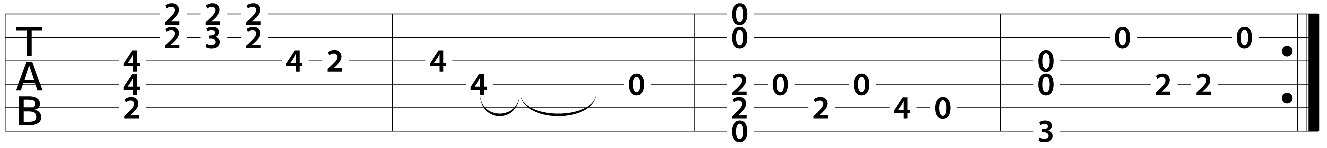
\includegraphics[width=350pt, height=40pt ]{res/islander.pdf}
\end{figure}
\verse{1}{}\Hm{}An old man by a \H[sus2]{}seashore \G[maj]{}at the end of day\\
\A{}gazes the \G{}horizon with \A{}seawinds in his \Hm{}face.\\
Tempest-tossed island, seasons all the same,\\
anchorage unpainted and a ship without a name.

\vskip -2ex
\verse{2}{}Sea without a shore for the banished one unheard,\\
he lightens the beacon, light at the end of world.\\
Showing the way, lighting hope in their hearts,\\
the ones on their travels homeward from afar.

\vskip -2ex
\chorus{}This is for \G{}long \D{}for - \A{}got - \Hm{}ten\\
\G{}light at the \D{}end of the \Em{}world\Hm{}.\\
Ho\G{}ri - \D{}zon \A{}cry - \Hm{}ing\\
the \G{}tears he left be\D{}hind long a\Em{}go.

\vskip -2ex
\verse{3}{}The albatross is flying, making him daydream,\\
the time before he became one of the world`s unseen.\\
Princess in the tower, children in the fields,\\
life gave him it all -- an island of the universe.

\vskip -2ex
\verse{4}{}Now his love's a memory, a ghost in the fog,\\
\textls[-30]{he sets the sails one last time saying farewell to the world.}\\
Anchor to the water, seabed far below,\\
grass still in his feet and a smile beneath his brow.\\
\textbf{R: }
}


\toftagthis{olympic}
\song{Jasná zpráva}{Olympic}{60pt}{1}{
\verse{1}{}\C{}Skončili jsme, jasná zpráva,\\
\Am{}proč o tebe \F{}zakopávám \G{}dál?\\
\Dm{}Projít bytem \F{}já abych se \C{}bál.

\verse{2} Dík tobě se vidím zvenčí,\\
připadám si starší, menší, sám.\\
Kam se kouknu, kousek tebe mám.

\chorus{}\Am{}Pěnu s vůní \Em{}jablečnou, \Am{}vyvanulý \Em{}sprej,\\
\Am{}telefon, cos \C{}ustřihla mu \G{}šnůru.\\
Knížku krásně zbytečnou, co má lživý děj,\\
píše se v ní, jak se lítá vzhůru,\\
lítá \Dm{}vzhůru, ve dvou \G{}vzhůru.

\verse{3}{}Odešlas mi před úsvitem,\\
mám strach bloudit vlastním bytem sám.\\
Kam se kouknu, kousek tebe mám.\\
\textbf{R:}

\verse{4}{}Skončili jsme, jasná zpráva,\\
není komu z okna mávat víc,\\
jasná zpráva, rub, co nemá líc.\\
\textbf{R:}

}


\toftagthis{nerez}
\song{Já s tebou žít nebudu}{Nerez}{45pt}{0.9}{
\verse{1}\Em{}Bylas jak poslední hlt \Fs{}vína,\\
\H[7]{}sladká a k ránu bola\Em{}vá, \hskip 0.8em \E[dim]{} \hskip 2.7em \H[7]{}\\
\Em{}za nehty výčitky a \Fs{}špína,\\
\H[7]{}říkalas: \uv{Dnešní noc je \Em{}tvá.}\hskip 0.3em \E[dim]{} \hskip 2.7em \H[7]{}

\chorus{}\G{}Co my dva z lásky vlastně \H{}máme,\\
\Am{}hlubokou \E[dim]{}šachtou padá \H[7]{}zdviž, já říkám \uv{kiš-kiš},\\
\Em{}navrch má vždycky těžký \Fs{}kámen\\
\H[7]{}a my jsme v koncích čím dál \Em{}blíž,\hskip 0.5em  \E[dim]{} \hskip 2.7em \H[7]{}\\
\revrpt{} \Em{}a me tu ha nadži vava \Am{}jaj dar\E[dim]{}i dari \H[7]{}daj. \rpt{}

\verse{2}Zejtra tě potkám za svým stínem,\\
neznámí známí v tramvaji,\\
v cukrárně kávu s harlekýnem,\\
hořká a sladká splývají.\\
\textbf{R:}

\verse{3}Bylas jak poslední hlt vína,\\
zbývá jen účet zaplatit a jít,\\
za nehty výčitky a špína\\
a trapný průchod banalit.

\chorus{}Co my tři z lásky vlastně máme,\\
hlubokou šachtou padá zdviž, co čumíš, kiš-kiš,\\
navrch má vždycky těžký kámen\\
a my jsme v koncích čím dál blíž,\\
\revrpt{} a me tu ha nadži vava jaj dari dari daj. \rpt{}

\revrpt{} \Em{}Navrch má vždycky těžký \Fs{}kámen\\
\H[7]{}a my jsme v koncích čím dál \Em{}blíž \hskip 0.5em \E[dim]{} \hskip 2.7em \H[7]{} \rpt{} $^{4\times}$\\
}


\toftagthis{zalman}
\song{Jdem zpátky do lesů}{Pavel Lohonka Žalman}{30pt}{1}{
\verse{1}\Am[7]{}Sedím na kolejích, \D[7]{}které nikam nevedou,\G{} \hskip 1em \C{} \hskip 1em \G{}\\
\Am[7]{}koukám na kopretinu jak \D[7]{}miluje se s lebe\G{}dou\C{}. \hskip 1em \G{}\\
\Am[7]{}Mraky vzaly slunce \D[7]{}zase pod svou ochra\G{}nu, \Em{}\\
\Am[7]{}jen ty nejdeš, holka zlatá, \D[7]{}kdypak já tě dosta\G{}nu?\D[7]{}

\chorus{}\G{}Z ráje, my vyhnaní \Em{}z ráje,\\
kde není už \Am[7]{}místa, \hskip 0.5em \C[7]{} prej něco se \G{}chystá.\D[7]{}\\
\G{}Z ráje nablýskaných \Em{}plesů\\
jdem zpátky do \Am[7]{}lesů, \hskip 0.5em \C[7]{}za nějaký \G{}čas. 

\verse{2}Vlak nám včera ujel ze stanice do nebe,\\
málo jsi se snažil, málo šel jsi do sebe.\\
Šel jsi vlastní cestou a to se zrovna nenosí,\\
i pes, kterej chce přízeň, napřed svýho pána poprosí.\\
\textbf{R:}

\verse{3}Už tě vidím z dálky, jak máváš na mě korunou\\
a jestli nám to bude stačit, zatleskáme na druhou.\\
Zabalíme všechny, co si dávaj' rande za branou,\\
v ráji není místa, možná v pekle se nás zastanou.\\
\textbf{R:}
}

\toftagthis{nohavica}
\song{Jdou po mně jdou}{Jaromír Nohavica}{55pt}{1}{
~\\
\verse{1}{}Býval jsem \D{}chudý jak \G{}kostelní \D{}myš,\\
\D{}na půdě \Fsm{}půdy jsem \Hm{}míval svou \A{}skrýš,\\
\revrpt{} \G{}pak jednou v \D{}létě \A{}řek' jsem si \Hm{}bať,\\
\G{} svět facku\D{}je tě a \G{}tak mu to \D{}vrať. \rpt{}

\verse{2}{}Když mi dát nechceš, já vezmu si sám,\\
zámek jde lehce a adresu znám,\\
\revrpt{} zlato jak zlato, dolar či frank,\\
tak jsem šel na to do National Bank. \rpt{}

\chorus{}Jdou po mně, \D{}jdou, \G{}jdou, \D{}jdou,\\
\D{}na každém \Fsm{}rohu ma\G{}jí fotku \A{}mou,\\
\G{}kdyby mě \D{}chytli, \A{}jó, byl by \Hm{}ring,\\
\G{}tma jako v \D{}pytli je v \C{}celách Sing-\G{}sing,\\
\A{}jé \D{}jéé\G{}. \hskip 0.8em \D{} \hskip 1em \CHORD{--}{}

\verse{3}{}Ve státě Iowa byl od poldů klid,\\
chudičká vdova mi nabídla byt,\\
\revrpt{} jó, byla to kráska, já měl peníze,\\
tak začla láska jak z televize. \rpt{}

\verse{4}{}Však půl roku nato řekla mi: \uv{Dost,\\
tobě došlo zlato, mně trpělivost,\\
\revrpt{} sbal svých pár švestek a běž si, kam chceš,}\\
tak jsem na cestě a chudý jak veš. \rpt{}\\
\textbf{R:}

\verse{5}{}Teď ve státě Utah žiju spokojen,\\
pípu jsem utáh' a straním se žen,\\
\revrpt{} jó, kladou mi pasti a do pastí špek,\\
já na ně mastím, jen ať mají vztek. \rpt{}

\chorus{}Jdou po mně \D{}jdou, \G{}jdou, \D{}jdou,\\
\D{}na nočních \Fsm{}stolcích ma\G{}jí fotku \A{}mou,\\
\G{}kdyby mě \D{}klofly, \A{}jó, byl by \Hm{}ring,\\
\G{}být pod pan\D{}toflí je \C{}hůř než v Sing-\G{}sing.\\
\A{}jé \D{}jéé\G{}. \hskip 0.8em \D{} \hskip 1em \CHORD{--}{}
}


\toftagthis{hlas}
\song{Jednou mi fotr povídá}{Ivan Hlas}{25pt}{1}{
\verse{1}\A[7]{}Jednou mi fotr povídá: \uv{\D[7]{}Zůstali jsme už sami dva,}\\
že \E{}si chce začít taky trochu ží\A[7]{}t.\\
\uv{Nech si to projít palicí a nevracej se s vopicí\\
snaž se mě hochu trochu pochopit.} 

\chorus{}Já \E{}šel, šel dál, baby, \A[7]{}kam mě Pán Bůh zval\\
já \E{}šel, šel dál, baby, a \D[7]{}furt jen tancoval.\\
Na \A[7]{}každý divný hranici, \D[7]{}na policejní stanici,\\
\E{}hrál jsem jenom rock'n'roll for you.\A[7]{}

\verse{2}Přiletěl se mnou černej čáp, zobákem dělal rock'n'klap\\
a nad kolíbkou Elvis Presley stál.\\
Obrovskej bourák v ulici, po boku krásnou slepici\\
a lidi šeptaj: \uv{Přijel nějakej král!}\\
\textbf{R:}

\verse{3}Pořád tak nějak nemohu chytit štěstí za nohu\\
a nemůžu si najít klidnej kout.\\
Blázniví ptáci začnou řvát a nový ráno šacovat\\
a do mě vždycky pustí silnej proud.\\
\textbf{R:}\\
}


\toftagthis{krestan}
\song{Jeruzalém ze zlata}{Pavlína Jíšová / Naomi Šemer}{17pt}{0.95}{
~\\
\verse{1}{}\A[ \noexport{$(\sfrac{3}{4})$}]{}Horský vzduch čistý jak \Dm[ \noexport{$(\sfrac{4}{4})$}]{}víno, ve větru \A[ \noexport{$(\sfrac{3}{4})$}]{}stmívání,\A[ \noexport{$(\sfrac{3}{4})$}]{}\\
\A{}přináší borovou \Dm{}vůni a ze všech \Am{}míst \E{}zvony \Am{}zní.\\
Ticho stromů a bílý kámen ve spánku objímá\\
to město až k bolesti krásné, co v srdci svém zeď má. 

\chorus{}Jeruza\Dm{}léme \G{}ze zla\C{}ta, z mědi a \F{}záře tajems\Am{}tví,\\
pohleď, i \F{}já jsem jeden \C{}z tónů \E{}všech \Am{}pí \hskip 0.2em - \hskip 0.2em s\E{}ní \Am{}tvých.\\
Jerušalajim šel zahav, vešel nechošet vešel or\\
halo lechol -- širjájich, ani kinor 

\verse{2}{}Smutek sedá na trh prázdný a k vyschlým cisternám,\\
\textls[-10]{jen lítost chodí starým městem k hoře, kde stával chrám.}\\
V jeskyních tisíc sluncí zhaslých jen vítr rozdmýchá,\\
nemohu jít k Mrtvému moři, nemohu jít do Jericha.\\
\textbf{R:}

\vskip -2ex
\verse{3}{}Ať mi jazyk můj na patro přilne a ruce neslouží,\\
\textls[-35]{když zapomenu tvoje jméno, budu pít hořkou vodu z kaluží.}\\
Jak sabra, která vprostřed pouště vždy znovu rozkvétá,\\
tak budu já o tobě zpívat, Jeruzaléme ze zlata.\\
\textbf{R:}

\vskip -2ex
\verse{4}{}Tak málokdy a přece zázrak, zeď je zhroucená,\\
šofar volá na horu chrámu, na trh a k plným cisternám.\\
V jeskyních tisíc sluncí září, až téměř nedýchám,\\
a mohu jít k Mrtvému moři a mohu jít do Jericha.\\
\textbf{R:}\\
}


\toftagthis{krestan}
\song{Ještě jedno kafe}{Robert Křesťan \& Druhá tráva}{25pt}{1}{
\verse{1}Máš \Em{}sladkej dech a oči, kterým \D{}patří svatozář,\\
\C{}a vlasy máš jak hedvábí, když je \H[7]{}hodíš na polštář,\\
ale já se o tvou lásku ani vděčnost neprosím,\\
ty děkuješ jen hvězdám a jseš věrná jenom jim. 

\chorus{}\C{}Ještě jedno kafe bych si \H[7]{}dal,\\
\C{}ještě jedno kafe, kruci\H[7]{}nál, než pojedu \Em{}dál. 

\verse{2}Tvůj táta, to je vandrák a od přírody zběh\\
a místo písmen učí tě jen dorovnávat dech,\\
a taky házet nožem a držet pospolu\\
a brada se mu třese, když se nosí ke stolu.\\
\textbf{R:} 

\verse{3}Tvá sestra hádá z ruky a tvá máti jakbysmet\\
a ty sama umíš všechno, co je mimo tenhle svět,\\
a tvá rozkoš nezná hranic, děvče s hlasem skřivana,\\
jen tvý srdce je jak moře -- samý tajemství a tma.\\
\textbf{R:}\\
}


\toftagthis{nohavica}
\song{Ježíšek}{Jaromír Nohavica}{30pt}{0.9}{
\crdheight=2.3ex
\verse{1}{}Dal sem na plotnu \Am{}vodu, zapnul \Dm{}plyn,\\
nasypal \G{}černou mletou kávu do \C{}hrníčku.\E{}\\
Pustil sem \Am{}desku -- trojku \Dm{}Queen,\\
zapálil \E{}na stromečku nejhořejší \Am{}svíčku.

\chorus{}\Am{}Na stěnách skotačí černé \Dm{}stíny,\\
nechytneš\E{} je, nepolapíš, je to \Am{}marné, když se trápíš.\\
Z vánočních koled jsou ever\Dm{}greeny\\
a co \E{}ty, Ježíšku, ještě \Am{}spíš.

\verse{2}{}Celý svět čeká na boží znamení\\
a On si zatím kdesi lítá v Mléčné dráze.\\
A dole v městě za Domem umění\\
jde Santa Claus převlečený za Dědu Mráze.\\
\textbf{R:}

\vskip -1ex
\verse{3}{}Pokojem voní čerstvé konopí,\\
z ledničky vytáhnul jsem kapra sněhuláka.\\
Až se mi celý roztopí,\\
z balkónu do tmy z plných plic si zahulákám.

Pa pa ra, pa pa ra paparara\ldots{}\emph{(melodie jako refrén)}

\textbf{R:}\\
}

\toftagthis{mladek}
\song{Jožin z bažin}{Ivan Mládek}{40pt}{1}{
\vskip 20pt

\verse{1}{}\Em{}Jedu takhle tábořit \H[7]{}Škodou 100 na \Em{}Oravu,\\
spěchám, proto riskuji, \H[7]{}projíždím přes \Em{}Moravu.\\
\D[7]{}Řádí tam to \G{}strašidlo, \D[7]{}vystupuje \G{}z ba\H[7]{}žin,\\
\Em{}žere hlavně Pražáky, \H[7]{}jmenuje se \Em{}Jo - \D[7]{}žin.\\
~\\
\chorus{}\G{}Jožin z bažin močálem se \D[7]{}plíží,\\
Jožin z bažin k vesnici se \G{}blíží,\\
Jožin z bažin už si zuby \D[7]{}brousí,\\
Jožin z bažin kouše, saje, \G{}rdousí.\\
\C{}Na Jožina z \G{}bažin, \D{}koho by to napa\G{}dlo,\\
\C{}platí jen a \G{}pouze \D{}práškovací leta\G{}dlo.\H[7]{}\\
~\\
\verse{2}{}Projížděl jsem dědinou cestou na Vizovice,\\
přivítal mě předseda, řek' mi u slivovice:\\
\uv{Živého či mrtvého Jožina kdo přivede,\\
tomu já dám za ženu dceru a půl JZD!}\\
\textbf{R:}
\clearpage
\verse{3}{}Říkám: \uv{Dej mi, předsedo, letadlo a prášek,\\
Jožina ti přivedu, nevidím v tom háček.}\\
Předseda mi vyhověl, ráno jsem se vznesl,\\
na Jožina z letadla prášek pěkně klesl.

\chorus{}Jožin z bažin už je celý bílý,\\
Jožin z bažin z močálu ven pílí,\\
Jožin z bažin dostal se na kámen,\\
Jožin z bažin -- tady je s ním ámen!\\
Jožina jsem dostal, už ho držím, johoho,\\
dobré každé lóve, prodám já ho do ZOO.\\
}


\toftagthis{zalman}
\song{Kdyby tady byla taková panenka}{Pavel Lohonka Žalman}{12pt}{1.05}{
\vskip 8pt
\textls[-25]{\verse{1}\revrpt{} \D{}Kdyby tady byla taková panenka,
\A[7]{}která by mě \D{}chtěla, \rpt{}\\
\revrpt{}\textls[-35]{ \G{}která by mě chtěla, \D{}syna vychovala,
\A[7]{}přitom pannou by\D{}la. }\rpt{}

\verse{2}\revrpt{} Kdybych já ti měla syna vychovati,
přitom pannou býti, \rpt{}\\
\revrpt{} ty by jsi mi musel kolébku dělati,
do dřeva netíti. \rpt{}

\verse{3}\revrpt{} Kdybych já ti musel kolébku dělati,
do dřeva netíti, \rpt{}\\
\revrpt{} ty bys mi musela košiličku šíti
bez jehly a nití. \rpt{}

\verse{4}\revrpt{} Kdybych já ti měla košiličku šíti
bez jehel a nití, \rpt{}\\
\hskip -1pt\revrpt{} ty by jsi mně musel žebřík udělati
až k nebeské výši. \rpt{}

\verse{5}\revrpt{} Kdybych já ti musel žebřík udělati
až k nebeské výši, \rpt{}\\
lezli bysme spolu, spadli bysme dolů, byl by konec všemu,\\
lezli bysme spolu, spadli bysme dolů,\\
byl by konec vše\Hm{}mu.\hskip 1em  \G{} \hskip 1em  \A[7]{} \hskip 1.5em \D{}}\\
}


\toftagthis{nohavica}
\song{Když mě brali za vojáka}{Jaromír Nohavica}{20pt}{0.86}{
\verse{1}{}\Am{}Když mě brali za vo\C{}jáka, \G{}stříhali mě doho\C{}la,\\
\Dm{}vypadal jsem jako \Am{}blbec, \E{}jak i všichni doko\F{}la,\\
-\G{}la, -\C{}la, -\G{}la, \Am{}jak i všichni \E{}doko\Am{}la.

\verse{2}{}Zavřeli mě do kasáren, začali mě učiti,\\
jak mám správný voják býti a svou zemi chrániti,\\
-ti, -ti, -ti a svou zemi chrániti.

\verse{3}{}Na pokoji po večerce ke zdi jsem se přitulil,\\
vzpomněl jsem si na svou milou, krásně jsem si zabulil,\\
-lil, -lil, -lil, krásně jsem si zabulil.

\verse{4}{}Když přijela po půl roce, měl jsem zrovna zápal plic,\\
po chodbě furt někdo chodil, tak nebylo z toho nic,\\
nic, nic, nic, tak nebylo z toho nic.

\verse{5}{}Neplačte, vy oči moje, ona za to nemohla,\\
mladá holka lásku potřebuje a tak si k lásce pomohla,\\
-la, -la, -la, tak si k lásce pomohla.

\verse{6}{}Major nosí velkou hvězdu, před branou ho potkala,\\
\textls[-10]{řek' jí, že má zrovna volný kvartýr, tak se sbalit nechala,}\\
-la, -la, -la, tak se sbalit nechala.

\verse{7}{}Co je komu do vojáka, když ho holka zradila,\\
\textls[-5]{na shledanou, pane Fráňo Šrámku, písnička už skončila,}\\
-la, -la, -la, jakpak se Vám líbila?\\
-la, -la, -la, no nic moc extra nebyla.\\
}


\toftagthis{chinaski}
\song{Klára}{Chinaski}{30pt}{0.9}{
\H{}Ná nanana\Gsm{}nanananananana \E{}ná \Em{}\\
\H{}Ná nanana\Gsm{}nanananananana \E{}ná aa\Em{}áá

\verse{1}\H{}Kláro, jak to s \Dsm{}tebou vypadá,\\
od půl \Csm{}devátý, do osmi \Em{}ráno,\\
co nám \H{}brání bejt spolu \Dsm{}jenom ty a já,\\
\Csm{}nebuď včerejší, no tak, \Em{}Kláro.

Pro tebe \H{}slibuju, žaluju, denně \Dsm{}piju jak Dán,\\
\Csm{}ve skrytu duše marně \Em{}tajně doufám,\\
že \H{}já, jenom \Gsm{}já jsem ten tvůj vysněný \E{}pán\ldots{}\Em{}\\
\H{}Ná nanana\Gsm{}nanananananana \E{}ná aa\Em{}áá

\verse{2}Já se prostě nekontroluju a plácám a plácám,\\
jsi vážně úžasná, já tě nejspíš miluju,\\
no ty mi dáváš, jééé!

Zabalit, vyrazit, rychle frčíme dál,\\
bereme čáru, šup do kočáru!\\
Já, jenom já jsem ten tvůj vysněný pán,\\
inženýr -- šarlatán.

\chorus{}\C{}Koukám na tebe, Kláro, už několik dní\Dm[7]{}, \hskip 2.5em \Db[maj]{}\\
nejsem nějakej ten chlápek, jsem solidní.\\
Kláro, stačí jen málo a budeme pár.\\
Královno má, ty to víš, co bych si přál.\\
\revrpt{} \C{}Ná nanana\Am{}nanananana\F{}naá aáá\Fm{}aáa \rpt{}

\verse{3}\C{}Hele, kotě, na co tě \Em{}nalákám?\\
\Dm{}Mám doma sbírku cinknu\Fm{}tejch srdcovejch králů,\\
\C{}naslouchám, následně \Em{}vím, kudy kam,\\
\Dm{}dáme si partičku a \Fm{}skončíme k \C{}ránu.

Počkám a\Em{}ž usneš\Dm{}\ldots{} \hskip 0.8em a \Fm{}budu se ti \C{}zdát,\\
jenom já \Am{}jsem ten tvůj vysněný \F{}pán,\\
inže\Fm{}nýr -- šarlatán.

\chorus{}\Cs{}Koukám na tebe, Kláro, už několik dní\Dsm[7]{}, \hskip 3em \D[maj]{}\\
nejsem nějakej ten chlápek, jsem solidní.\\
Kláro, stačí jen málo a budeme pár.\\
Královno má, ty to víš, co bych si přál.

\Cs{}Ná nananananananana\Dsm[7]nááá áá\D[maj]{}á\\
Ná nananananananananááá ááá\\
\Cs{}Ná nananananananana\Dsm[7]{}ná nanana\D[maj]{}nanananá ná \Cs{}nááá\\
}


\toftagthis{vw}
\song{Klobouk ve křoví}{J. Ježek / V+W}{100pt}{0.93}{
\crdheight=2.2ex
\verse{1}{}\C{}Vítr \Bb[9]{}vane \C{}pouští,\G[+7]{}\\
\C{}po písku \Bb[9]{}žene klo\C{}bouk,\C[7]{}\\
\Fm{}zahnal \G[7]{}ho do \C{}houští,\Am{}\\
\Fm{}starý a \G[7]{}černý klo\C{}bouk.\G[7]{}

\vskip -1ex
\verse{2}{}Kdepak je ta hlava,\\
která klobouk nosila?\\
\F{}Byla čer\G[7]{}ná či \C{}plavá?\Am{}\\
\Fm{}Komu a\G[7]{}si patři\C{}la? \Am{}

\vskip -1ex
\verse{3}{}\Em{}Kdo to v poušti \F{}zmizel?\\
\Em{}Odkud šel a \A[7]{}kam?\\
\G{}Jaký to měl \A[dim]{}svízel,\\
\G{}že byl v \F[7]{}pou\Gb[7]{}šti \hskip 1em \G[7]{}sám?\G[+7]{}

\vskip -1ex
\verse{4}{}\C{}Jen za\Ab{}váté \C{}stopy,\G[+7]{}\\
\C{}starý klo\Bb[9]{}bouk ve křo\A[7]{}ví.\\
\Dm{}Nikdo nic \G[7]{}nepo\C{}chopí,\\
\Fm{}nikdo se \Ab[7]{}nic \hskip 1em \Ab[7]{}ne - \G[7]{}do - \C{}ví. \hskip 0.3em \C[6]{}\\
}


\toftagthis{anglicke}
\song{Knockin' on Heaven's Door}{Bob Dylan}{50pt}{1}{
\verse{1}{}\G{}Mama, \D{}take this badge of \Am{}me,\\
\G{}I can't \D{}use it any\C{}more.\\
It's getting dark, too dark to see,\\
feels like I'm knockin' on heaven's door.

\chorus{}Knock, knock, knockin' on heaven's door\\
Knock, knock, knockin' on heaven's door\\
Knock, knock, knockin' on heaven's door\\
Knock, knock, knockin' on heaven's door\\
~\\
\verse{2}{}Mama, put my guns in the ground,\\
I can't shoot them anymore.\\
That cold black cloud is comin' down,\\
feels like I'm knockin' on heaven's door.\\
\textbf{R: $(2\times)$}
}


\toftagthis{hapka}
\song{Kocour se schoulil na tvůj klín}{Petr Hapka / Michal Horáček}{80pt}{1}{
\verse{1}Kocour se schoulil na tvůj \C{}klín,\\
u nohou \G[/H]{}spí ti dalma\Am{}tin, \hskip 1em \G[/H]{}\\
\C{}v pozicí lvů co \C[/E]{}zdobí \F[add9]{}banku,\\
i sama noc má na ka\C[/E]{}hánku,\\
jen ty se ještě ještě bráníš \Dm{}spánku\\
a \D[sus4]{}síle \hskip 2em \Am{}starých \G{}vín.

\verse{2}Jak dlouho to však vydržíš?\\
Už na kostele zlátne kříž,\\
ne, ani jeho svatá záře\\
nenajde důlek do polštáře,\\
natožpak obrys mužské tváře,\\
a ty to dobře víš.

\chorus{}Má \F[add9]{}krásko, s přetěžkými \C{}víčky,\\
\F[add9]{}snad je tvůj rytíř na ces\C{}tách,\\
\F[add9]{}snad si tvou krajkou \C{}od spodnič\Am{}ky\\
stírá \Dm{}prach, \G{} na ces\C{}tách.

\verse{3}Až přes řeku a do strání\\
se rozléhá tvé volání,\\
i Jonáš ve velrybím břiše\\
by tvoje slova musel slyšet,\\
vždyť voláš tišeji než tiše,\\
kdo se ti ubrání.

\verse{4}Vidíš však, nebo nevidíš,\\
už na kostele zlátne kříž,\\
ne, ani jeho svatá záře\\
nenajde důlek do polštáře,\\
natožpak obrys mužské tváře,\\
a den je blíž a blíž.

\chorus{}Má krásko, s přetěžkými víčky,\\
kývou se, kývou, misky vah,\\
na jedné krajka od spodničky,\\
na druhé, na druhé víří prach.

\verse{5}I ve zvířeném prachu cest\\
vidím tě lampu k oknu nést,\\
tvá silueta ale bledne,\\
kdo pohlédne, už nedohlédne,\\
snad ještě můra k lampě sedne,\\
já však znám tu lest.

\chorus{}Má krásko, s přetěžkými víčky,\\
i když má víčka tíží prach,\\
tak po tvé krajce od spodničky\\
teď -- bych už nerad sáh.
}

\toftagthis{nohavica}
\song{Kometa}{Jaromír Nohavica}{35pt}{1}{
\verse{1}{}\Am{}Spatřil jsem kometu, oblohou letěla,\\
chtěl jsem jí zazpívat, ona mi zmizela,\\
\Dm{}zmizela jako laň \G[7]{}u lesa v remízku,\\
\C{}v očích mi zbylo jen \E[7]{}pár žlutých penízků.

\verse{2}{}Penízky ukryl jsem do hlíny pod dubem,\\
až příště přiletí, my už tu nebudem,\\
my už tu nebudem, ach, pýcho marnivá,\\
spatřil jsem kometu, chtěl jsem jí zazpívat.

\chorus{}\Am{}O vodě, o trávě, \Dm{}o lese,\\
\G[7]{}o smrti, se kterou smířit \C{}nejde se\E[7]{},\\
\Am{}o lásce, o zradě, \Dm{}o světě\\
\textls[-15]{\E{}a o všech lidech, co kdy \E[7]{}žili na téhle \Am{}planetě\Dm{}. \hskip 2em \E[7]{}}

\verse{3}{}Na hvězdném nádraží cinkají vagóny,\\
pan Kepler rozepsal nebeské zákony,\\
hledal, až nalezl, v hvězdářských triedrech\\
tajemství, která teď neseme na bedrech.

\verse{4}{}Velká a odvěká tajemství přírody,\\
že jenom z člověka člověk se narodí,\\
\clearpage
\leftskip 50pt
že kořen s větvemi ve strom se spojuje\\
a krev našich nadějí vesmírem putuje.\\
\chorus{}Na na na\ldots{}

\verse{5}{}Spatřil jsem kometu, byla jak reliéf\\
zpod rukou umělce, který už nežije,\\
šplhal jsem do nebe, chtěl jsem ji osahat,\\
marnost mne vysvlékla celého donaha.

\verse{6}{}Jak socha Davida z bílého mramoru\\
stál jsem a hleděl jsem, hleděl jsem nahoru,\\
až příště přiletí, ach, pýcho marnivá,\\
my už tu nebudem, ale jiný jí zazpívá.

\chorus{}O vodě, o trávě, o lese,\\
o smrti, se kterou smířit nejde se,\\
o lásce, o zradě, o světě,\\
bude to písnička o nás a kometě.\\
}

\toftagthis{nohavica}
\song{Kozel}{Jaromír Nohavica}{70pt}{1}{
~\\
\verse{1}{}Byl jeden \G{}pán, ten kozla \C{}měl,\\
velice \D{}si s ním rozu\G{}měl.\\
Měl ho moc rád, opravdu moc,\\
hladil mu fous na dobrou noc.

\verse{2}{}Jednoho dne se kozel splet,\\
rudé tričko pánovi sněd.\\
Jak to pán zřel, zařval: \uv{Jéjé!},\\
svázal kozla na koleje.

\verse{3}{}Zapískal vlak, kozel se lek'.\\
\uv{To je má smrt,} mečel, \uv{mek, mek!}\\
Jak tak mečel, vykašlal pak\\
rudé tričko, čímž stopnul vlak.

Ná ná ná na\ldots{}
}

\toftagthis{filmove}
\song{Kujme pikle}{Šíleně smutná princezna}{80pt}{1}{
\capo{3}
\verse{1}\Em{}Kujme \Em[/F$\sharp$]{}pikle, \hskip 1em \Em[/G]{}kujme \hskip 0.5em \Em[/F$\sharp$]{}pikle,\\
\Em{}obvy - \Em[/G]{}klé \hskip 0.5em i \hskip 0.5em  \Am[/F$\sharp$]{}neobvy - \H[7]{}klé.\\
Kujme pikle, pikle kujme,\\
snad se pikle s piklí ujme.\\
\Am{}Budeme \Em{}pikliti\\
\Am{}za krá\Am[/F$\sharp$]{}lovské \hskip 1em \H[7]{}ti - ti - \Em{}ti. \hskip 1em \H[7]{}

\verse{2}Kujme pikle, kujme pikle,\\
správná pikle lidi zvikle.\\
Kujme pikle, pikle kujme,\\
intrikujme, spekulujme.\\
Lepšího nic není\\
nad pořádný piklení.

\verse{3}Hledá vězně, však my víme,\\
a my jí to překazíme.\\
V tom vám musím odporovat,\\
my to budem podporovat.\\
\revrpt{} \Am{}Vlákáme ji \Em{}do sítí\\
a \H[7]{}budem dále \Em{}pikliti. \rpt{} $^{3\times}$\\
}



\toftagthis{nohavica}
\song{Ladovská zima}{Jaromír Nohavica}{30pt}{1}{
\capo{5}
\verse{1}
\C[add9]{}Za vločkou vločka\G[6]{} z oblohy padá,\\
\D[sus2/F$\sharp$]{}chvilinku počká\G[6]{} a potom taje.\\
Na staré sesli sedí pan Lada,\\
obrázky kreslí zimního kraje.

\chorus{}Ladovská zima za okny je\\
a srdce jímá bílá nostalgie,\\
ladovská zima, děti a sáně,\\
a já jdu s nima do chrámu Páně.\\
Bim bam bim bam bim bam\\
bim bam bim bam bim.

\rec{To mokré bílé svinstvo padá mi za límec,\\
už čtvrtý měsíc v jednom kuse furt prosinec.\\
Večer to odhážu, namažu záda,\\
ráno se vzbudim a zas kurva padá.\\
Děcka majú zmrzlé kosti,\\
sáňkujú už jenom z povinnosti.\\
Mrzne jak sviňa, třicet pod nulu,\\
auto ani neškytne, hrudky se dělají v Mogulu.\\
Kolony aut, krok, sun, krok,\\
bo silničáři, tak jak každý rok,\\
jsou překvapeni velice,\\
že sníh zasypal jim silnice.\\
Pendolino stojí kdesik u Polomi,\\
zamrzly mu všecky CD-ROMy.\\
A policajti? Ti to jistí z dálky,\\
zalezlí do Aralky.}\\
\textbf{R:}

\rec{Na Vysočině zavřeli Dé jedničku,\\
kamiony hrály na honičku,\\
tzv. rallye Letní gumy,\\
v tym kopcu u Meziříčí,\\
spěchali s melounama a teď jsou v… (však víte kde).\\
Na ČT1 Studio sníh,\\
Voldanová sedí na saních.\\
A v Praze kalamita jak na Sibiři,\\
tři centimetry sněhu a u Muzea čtyři.\\
Jak v dálce vidím zasněžený Říp,\\
říkám si: Praotče Čechu, tys byl ale strašný cyp.\\
Kdyby jsi popošel ještě o pár kilometrů dále,\\
tak jsem se teďka mohl kdesi v teple v plavkách válet.\\
Místo toho aby se člověk bál zajít do Tesca na nákupy,\\
jak jsou tam na tych rovných střechách sněhu kupy.\\
Do toho všeho jak mám zmrzlý nos aj líca,\\
tak ještě z rádia provokatér Nohavica.\\}
\textbf{R:}
}


\toftagthis{kryl}
\song{Lásko}{Karel Kryl}{45pt}{0.95}{
\verse{1}\Am{}Pár zbytků pro krysy na misce od guláše,\\
\E{}milostný dopisy, s partií\Dm{} mariáše.\\
Před cestou dalekou zpocený boty zujem\\
\C{}a potom pod dekou \E{}sníme, když onanujem.

\vskip -2ex
\chorus{}\Am{}Lásko, \G{}zavři se do pokoje,\\
\Am{}lásko, \G{}válka je holka moje,\\
s \C{}ní se \G{}milu\Am{}ji, když \G{}noci si \Am{}krátím\E{}.\\
Lásko, slunce máš na vějíři,\\
lásko, dvě třešně na talíři,\\
ty ti daruji, až jednou se vrátím.

\verse{2}Dvacet let necelých, odznáček na baretu,\\
s úsměvem dospělých vytáhnem cigaretu,\\
v opasku u boku nabitou parabelu,\\
zpíváme do kroku pár metrů od bordelu.\\
\textbf{R:}

\verse{3} Pár zbytků pro krysy a taška na patrony,\\
latrína s nápisy, jež nejsou pro matróny,\\
není čas na spaní, smrtka nám drtí palce,\\
nežli se zchlastaní svalíme na kavalce.\\
\textbf{R:} Levá, dva!\\
\textbf{R:}\\
}


\toftagthis{filmove}
\song{Lásko má, já stůňu}{Karel Svoboda}{25pt}{1}{
\capo{4}

\verse{1}{}\Am{}Já, ač mám spánek \Em{}bezesný, mně \D{}včera \E{}sen se \Am{}zdál.\\
\Am{}I když dávno \Em{}nejsem s ním, mě \D{}navští\E{}vil sám \F{}král, \G{}řekl:

\chorus{}\uv{\C{}Lásko má, já \G{}stůňu, svoji \Dm{}pýchu já jen \Am{}hrál,\\
kvůli \C[7]{}vám se vzdávám \F{}trůnu, kleno\C{}tů i \G{}kate\E{}drál.}

\verse{2}{}Ač den mám jindy poklidný, dnes nevím, kudy kam.\\
Trápí mě sen ošidný a trápí mě král sám, řekl:

\chorus{}\uv{Lásko má,\ldots{}\\
\hskip 1em \ldots{}klenotů i kate\C{}drál.} \G{}Řekl:

\chorus{}\uv{Lásko má,\ldots{}\\
\hskip 1em \ldots\ klenotů i kate\A{}drál.}\\
}


\toftagthis{anglicke}
\song{Leaving on a Jet Plane}{John Denver}{50pt}{1}{
\verse{1}All my \C{}bags are packed, I'm \F{}ready to go,\\
I'm \C{}standing here out\F{}side your door,\\
I \C{}hate to wake you \F{}up to say good\G{}bye. 

\verse{2}But the dawn is breaking, it's early morn,\\
the taxi's waiting, he's blowing his horn,\\
already, I'm so lonesome I could die. 

\chorus{}So kiss me and smile for me,\\
tell me that you'll wait for me,\\
hold me like you'll never let me go. 

'Cause I'm leaving on a jet plane,\\
don't know when I'll be back again,\\
oh, babe, I hate to go. 

\verse{3}{}There's so many times I've let you down,\\
so many times I've played around,\\
I tell you now they don't mean a thing. 

\verse{4}Every place I'll go I think of you,\\
every song I sing I'll sing for you,\\
when I come back,  I'll bring your wedding ring.\\
\textbf{R:} 
\clearpage
\verse{5}{}Now the time has come to leave you,\\
one more time let me kiss you,\\
then close your eyes, I'll be on my way. 

\verse{6} Dream about the days to come,\\
when I won't have to leave alone,\\
about the times, I won't have to say.\\
\textbf{R: + $\downarrow$}

I'm leaving on a jet plane,\\
don't know when I'll be back again,\\
oh, babe, I hate to go.\\
}


\toftagthis{anglicke}
\song{Lemon Tree}{Fool's Garden}{30pt}{1}{
\verse{1}{}I'm \Dm{}sittin' here in the \Am{}boring room,\\
it's just another rainy Sunday afternoon,\\
I'm wasting my time, I got nothing to do,\\
I'm hangin' around, I'm waitin' for you\\
but \Gm{}nothing ever happens\Am{} -- and I \Dm{}wonder.

\verse{2}{}I'm drivin' around in my car,\\
I'm drivin' too fast, I'm drivin' too far,\\
I'd like to change my point of view,\\
I feel so lonely, I'm waiting for you\\
but nothing ever happens -- and I wonder.

\chorus{}I \F{}wonder how, \C{}wonder why\\
\Dm{}yesterday you told me 'bout the \Am{}blue blue sky\\
and \Bb{}all that I can \C{}see\\
is just a yellow \F{}lemon tree\C{}.\\
I'm \F{}turnin' my head \C{}up and down,\\
i'm \Dm{}turnin' turnin' turnin' turnin' \Am{}turnin' around\\
and \Bb{}all that I can \H[dim]{}see\\
is just a yellow \C{}lemon tree\C[7]{}.

Ta, da da didap\ldots{}

\verse{3}{}I'm sittin' here, I miss the power,\\
I'd like to go out, takin' a shower\\
but there's a heavy cloud inside my head,\\
I feel so tired, put myself into bed\\
Where nothing ever happens -- and I wonder.

\verse{*}{}\A{}Isolation \Dm{}is not good for me,\\
\C{}isolation -- \F{}I don't want to \A{}sit on a lemon tree.

\verse{4}{}I'm steppin' around in a desert of joy,\\
baby, anyhow I get another toy\\
and everything will happen -- and you'll wonder.\\
\textbf{R: + $\downarrow$}

I \F{}wonder how, \C{}wonder why\\
\Dm{}yesterday you told me 'bout the \Am{}blue blue sky\\
and \Bb{}all that I can \C{}see\\
and \Bb{}all that I can \C{}see\\
and \Bb{}all that I can \C{}see\\
is just a yellow \F{}lemon tree.\\
}

\toftagthis{anglicke}
\song{Let It Be}{The Beatles}{55pt}{0.9}{
\verse{1}{}When I \C{}find myself in \G{}times of trouble,\\
\Am{}Mother Mary \F{}comes to me\\
\C{}speaking words of \G{}wisdom -- let it \F{}be.\C{} \hskip 0.8em \Dm{} \hskip 2em \C{}\\
And in my hour of darkness\\
she is standing right in front of me,\\
speaking words of wisdom -- let it be.

\chorus{}Let it \Am{}be, let it \G{}be, let it \F{}be, let it \C{}be,\\
\C{}whisper words of \G{}wisdom -- let it \F{}be. \C{} \hskip 0.8em \Dm{} \hskip 2em \C{}

\verse{2}{}And when the broken-hearted people\\
living in the world agree,\\
there will be an answer -- let it be.\\
For though they may be parted\\
there is still a chance that they will see,\\
there will be an answer -- let it be.

\chorus{}Let it be, let it be, let it be, let it be,\\
there will be an answer -- let it be.\\
Let it be, let it be, let it be, let it be,\\
whisper words of wisdom -- let it be.\\
Let it be, let it be, let it be, let it be,\\
there will be an answer -- let it be.\\
~\\
\F{} \hskip 1em \C{} \hskip 0.8em \Dm{} \hskip 2em \C{} \hskip 2em \Bb{} \hskip 1em \F[/A]{} \hskip 1.8em \G{} \hskip 1.5em \F{} \hskip 1.5em \C{}\\

\verse{3}{}And when the night is cloudy\\
there is still a light that shines on me,\\
shine on 'till tomorrow -- let it be.\\
I wake up to the sound of music,\\
Mother Mary comes to me\\
there will be no sorrow -- let it be.

\chorus{}Let it be, let it be, let it be, let it be,\\
there will be no sorrow -- let it be.\\
Let it be, let it be, let it be, let it be,\\
whisper words of wisdom -- let it be.
~\\
\F{} \hskip 1em \C{} \hskip 0.8em \Dm{} \hskip 2em \C{} \hskip 2em \Bb{} \hskip 1em \F[/A]{} \hskip 1.8em \G{} \hskip 1.5em \F{} \hskip 1.5em \C{}\\

}

\toftagthis{anglicke}
\song{Lion Sleeps Tonight}{The Tokens}{60pt}{1}{
\capo{1}
~\\
\verse{1}\E{}In the jungle, the \A{}mighty jungle,\\
the \E{}lion sleeps to\H{}night.\\
In the jungle, the quiet jungle,\\
the lion sleeps tonight.

\verse{2}Near the village, the peaceful village,\\
the lion sleeps tonight.\\
near the village, the quiet village,\\
the lion sleeps tonight.

\verse{3}Hush my darling, don't fear my darling,\\
the lion sleeps tonight.\\
Hush my darling, don't fear my darling,\\
the lion sleeps tonight.\\
}


% NEW SONGS
\toftagthis{sverakuhlir}
\song{Lotr intelektuál}{Z. Svěrák / J. Uhlíř}{40pt}{1}{
\medskip
\rec{Vykoupat! Odvšivit! Učesat! Voblíct!\\
Ráno půjde do školy!\\
Tu nejlepší školu mu dám! (Správně!)\\
Protože na to mám! (Správně!)}

\verse{1}\Am{}Dáme klukovi ško\Em{}ly,\hskip 1.2em \F{}ať to stojí coko\C{}li,\\
\G{}nešetříme na chlap\C{}ci, \F{}táto, \C{}šáhni \G{}do kap\C{}sy.

Když zná lupič písmena, stane se s ním proměna,\\
když zná lupič dějiny, tak je úplně jiný.

\chorus{}\C{}Bude \F{}to ozdoba \C{}loupežnické \G{}bandy,\\
\C{}bude \F{}mít brejličky \C{}a možná i \G{}kšandy,\\
\C{}posu\F{}ne řemeslo \C{}zas o kousek \G{}dál,\\
\C{}bude to \F{}lotr \G{}intelektu\C{}ál.

\verse{2}Naučí se francouzsky, bude nosit licousky,\\
naučí se mluvnici, \uv{přelstí všecky pravnici.}

Naučí se německy, řekne troky, ne necky,\\
když bude mluvit plynně, může loupit v cizině.\\
\textbf{R:}\\	
}



\toftagthis{ceskekapely}
\song{Magdaléna}{Jelen}{40pt}{1}{
\verse{1}\A{}Zapal ten oheň ve mně,\D[add9]{} čeho se bojíš,\\
\A{}zápalkou škrtni jemně\D[add9]{}.\\
Zapal ten oheň ve mně, čeho se bojíš,\\
zimou se celá třeseš, proč venku stojíš?\\
Pojď \A{}dál, prosím tě, \D[add9]{}nenech se prosit se \A{}dál,\\
\D[add9]{}nenech se! 

\verse{2}Sedíme na pavlači, přichází ráno,\\
tobě se lesknou oči.\\
Sedíme na pavlači, přichází ráno\\
a mně se hlava točí.\\
Pojď dál, prosím tě, nenech se prosit se dál,\\
nenech se! 

\chorus{}\Fsm{}Hodiny se zastaví a v \E{}devět třicet v pondělí,\\
\A{}Magdaléno, \A{}tvoje vlasy\\
leží pod mou postelí a i když jsme to nechtěli,\\
oblíkáš se, pročpak asi.\\
Hodiny se zastaví a v devět třicet v pondělí\\
jsem\A{} sám.\D[add9]{}
\clearpage
\verse{3}Stojíme na rozcestí a zvony zvoní,\\
daleko od bolestí.\\
Stojíme na rozcestí a zvony zvoní,\\
možná nás čeká štěstí.\\
Pojď dál, prosím tě, nenech se prosit se dál,\\
nenech se!\\
\textbf{R:}

\chorus{}Hodiny se zastaví a v devět třicet v pondělí,\\
Magdaléno, tvoje vlasy,\\
leží pod mou postelí a i když jsme to nechtěli,\\
oblíkáš se, pročpak asi.\\
Hodiny se zastaví a v devět třicet v pondělí\\
máš těžký srdce a mokrý řasy,\\
když vycházíš ze dveří, tak sama tomu nevěříš,\\
nenech se!\\
}


\toftagthis{kabat}
\song{Malá dáma}{Kabát}{80pt}{0.955}{
\verse{1}\Am{}Utrhla trávu a začla \D[sus2]{}hrát,\\
ta malá dáma z předměs\F{}tí,\\
co umí \E[7]{}lidem z dlaní \Am{}číst.\\
Tam kočky z rána mívaj' hlad,\\
po noci plný neřestí\\
je pohladí a dá jim jíst.

\verse{*}\Dm{}Po tmě se \D[sus2]{}toulá a ve dne \Am{}spí\\
a její oči vědí víc než \Dm{}mý,\\
došly mi \D[sus2]{}slova, já stál tam \F{}jen,\\
s touhle \E[7]{}jedinou bych \Am{}zemřel.

\chorus{}\Am{}S touhle bych \F{}zemřel v jedinej \C{}den\\
a jestli \E[7]{}vám to\E[7sus4]{} ne - sta - \Am{}čí,\\
kdyby tam \F{}stála stovka \C{}žen,\\
vyzvu ji \E[7]{}k tanci, a to \E[+]{}netan\Am{}čím.

\verse{2}Tam za tratí svý doupě má,\\
mince po kašnách posbírá\\
a pak je skládá na kolej.\\
Staví si chrám, plechovej most,\\
už po něm kráčí první host,\\
tak ať ho nohy nebolej.

\verse{*}Prošla si peklem a kouzla zná,\\
přejetý mince počítá\\
a kdo ji spatří je zatracen,\\
s touhle jedinou bych zemřel.\\
\textbf{R:}


\hskip -7pt \verse{\Large Br}Budu si \Am{}pamatovat na tu \C{}chvíli,\\
když hrála, \F{}znělo to jak Paga\E[7]{}nini.\\
A já už \Am{}věděl, že jsem ztrace\C{}nej,\\
zeptal se \F{}za kolik, s pocitem \E[7]{}viny.\\
\textbf{R: ($2\times$)}
}


\toftagthis{nohavica}
\song{Malé české blues}{Jaromír Nohavica}{40pt}{1}{
\verse{1}{}Koupil jsem \Dm{}kozu, nemám kozu,\\
včera mi \G{}pošla na virozu,\\
kdybych koupil \Bb{}kozla, taky by mi \A{}chcip,\\
takový jsem \Dm{}cyp. \hskip 0.3em \A{}Do prdele práce!

\verse{2}{}Třešeň v rohu zahrady roky mi nesla,\\
letos úroda na polovinu klesla,\\
že prý špačci, já ti dám špačci,\\
snědí spoluobčané. Do prdele práce!

\verse{3}{}Dřu jak mezek ve zbrojovce,\\
ve volném čase za barákem chovám ovce,\\
Neuwirt chová rybky v akváriu,  má na kontě mega\\
a já nic. Do prdele práce!

\verse{4}{}Moje stará, škoda slov,\\
takový malý Suvorov,\\
jak mi liskne tak to třiskne jak když o traverzu\\
buchne těžký kov. Do prdele práce!\\
\clearpage
\verse{5}{}Starší dcera robí v Londonderry,\\
mladší čeká děcko, ale neví s kerym,\\
synek sedí, bo byl hlupy,\\
nechal se chytit. Do prdele práce!

\verse{6}{}Topolánek, jasné jak facka,\\
jezdí v plavkách do Chorvatska,\\
já tak možu na horní splav do Lidečka,\\
tečka. Do prdele práce!

\verse{7}{}Na posraného i hovno padá,\\  
tady je těžká jaká smysluplná rada,\\
nejlepší bude odložit bendžo a zajít na jedno.\\
Do restaurace --  tak já jdu.\\
}


\toftagthis{ceskekapely}
\song{Malování}{Divokej Bill}{20pt}{0.82}{
\crdheight=2.2ex
\verse{1}\Dm{}Nesnaž se, \Dm{}znáš se,\Bb{} řekni mi, \C{}co je jiný,\\
\Dm{} jak v kleci máš se\Bb{} \hskip 1.2em \C{}pro nevinný,\\
\Dm{}noci dlouhý \Bb{}jsou plný \C{}touhy a \Dm{}lásky nás dvou. \Bb{}\\
\C{}Všechno hezký \Dm{}za sebou mám,\Bb{} můžu \C{}si za to \Dm{}sám,\\
\Bb{} v hlavě \C{}hlavolam,\\
\Dm{}jen táta a máma\Bb{} jsou s \C{}náma, \Dm{}napořád s náma.\Bb{}

\vskip -2ex
\chorus{}To \C{}je to tvoje \Dm{}malování \Bb{}vzdušnejch z\C{}ámků,\\
\Dm{}malování po \Bb{}zdech holejma \C{}rukama tě \Dm{}nezachrání,\\
už \Bb{}máš na ka\C{}hánku, \Dm{}nezachrání, už jsi \Bb{}na zá\C{}dech,\\
je to \Dm{}za náma, ty čteš \Bb{}poslední str\C{}ánku,\\
\Dm{} za náma,\Bb{} na \C{}zádech, \Dm{}za náma, už \Bb{}máš na ka\C{}hánku,\\
mezi\Dm{} náma,\Bb{} mi taky \Gm{}došel \Am{}dech\ldots{} 

\Dm{} \hskip 2.1em \Bb{} \hskip 1.2em \C{} \hskip 1em \Dm{} \hskip 2.1em \Bb{} \hskip 1.2em \Gm{} \hskip 2em \Am{}\\
\textbf{R:}

\verse{2}Znáš se, řekni mi, co je jiný, jak v kleci máš se,\\
pro nevinný noci dlouhý jsou plný touhy a lásky nás tří.
}


\toftagthis{buty}
\song{Mám jednu ruku dlouhou}{Buty}{65pt}{0.85}{
\crdheight=2.2ex
\hskip 3em \revrpt{} \E{}Na \Csm{}nananana \A{}ná \E{}ná \rpt{}

\verse{1}{}\E{}Najdem si \Csm{}místo, \Gsm{}kde se dobře \Fsm{}kouří,\\
kde horké slunce do nápojů nepíchá,\\
\H{}kde vítr \H[/A]{}snáší \E{}šmolky ptačích \A{}hovínek\\
\H{}okolo \A{}nás a \H{}říká\ldots{}

\verse{2}{}Můžeme zkoušet, co nám nejvíc zachutná,\\
tak klidně se dívat jestli někdo nejde,\\
někdo, kdo ví, že už tady sedíme,\\
a řekne: \uv{Nazdar, kluci.}\\
\chorus{}\revrpt{} \E{}Mám \Csm{}jednu ruku \A{}dlou\E{}hou. \rpt{}

\verse{3}{}\A{}Posaď se \Fsm{}k nám, \Csm{}necháme tě \Hm{}vymluvit\\
a vzpomenout si na ty naše úkoly.\\
\E{}Tu ruku nám \Hm{}dej a \A{}odpočívej \D{}v pokoji \E{} \hskip 1em \E{} \\
\A{}tam na tom \Fsm{}místě, \Csm{}kde se dobře \Hm{}není. \E{} \hskip 1em \Fermataup{4}

\chorus{}\revrpt{} \A{}Na, \Fsm{}nananana \D{}ná \A{}ná \rpt{} $^{4\times}$\\
\revrpt{} \Am{}Na nananana \rpt{} $^{3\times}$  \D{}ná \A{}ná\\
\revrpt{} \A{}Mám \Fsm{}jednu ruku \D{}dlou\A{}hou. \rpt{} $^{4\times}$\\
}


\toftagthis{nohavica}
\song{Mám jizvu na rtu}{Jaromír Nohavica}{35pt}{0.83}{
\crdheight=2.3ex
\hskip 1em \revrpt{} \textsf{\bfseries Cadd9\ \ Gsus2/H\ \   Fsus2\ \ Gsus4 } \rpt{}

\verse{1}{}\C[sus2]{}Jsem příliš starý na to, abych věřil v revoluci,\\
\G[sus4]{}a svoji velkou hlavu \G{}těžko skryju \G[sus4]{}pod kapuci\\
\Am[7]{}a nechutná mi, když se \F[sus2]{}vaří předvařená rýže,\\
\C[sus2]v náprsní kapse nosím\G[sus4]{} Ventinol \G{}na potíže.

\vskip -2ex
\chorus{}\Am[7]{}Jak to tak vidím, asi těžko projdu \Am[7/E]{}uchem jehly\\
\F[sus2]{}a lesem běhám tak, a\C[sus2]{}by mě vlci nedoběhli,\\
\Dm[7]{}a kdyby se někdo z vás na anděla \C[/E]{}ptal,\\
tak \C[sus2]{}mám jizvu na rtu,\G[sus4]{} když při mně stál.

\verse{2}{}Sako mám od popílku, na kravatě saze,\\
mé hrubé prsty neumí uzly na provaze\\
a když mi občas tečou slzy, hned je polykám\\
a tančím jen tak rychle, jak hraje muzika.

\vskip -2ex
\chorus{}Mé oči mnohé viděly a ruce mnohé měly\\
a srdce stydělo se, když salvy slávy zněly,\\
a kdyby se někdo z vás na anděla ptal,\\
tak mám jizvu na rtu, když při mně stál.

\verse{3}{}Mluvil jsem s prezidenty, potkal jsem vrahy,\\
nahý jsem na svět přišel a odejdu nahý,\\
v patnácti viděl jsem, jak kolem jely ruské tanky,\\
a v padesáti nechával si věštit od cikánky.

\vskip -2ex
\chorus{}A dříve, než mě přijme svatý Petr u komise,\\
básníkům české země chtěl bych uklonit se\\
a kdyby se někdo z vás na anděla ptal,\\
tak mám jizvu na rtu, když při mně stál.

\verse{4}{}V Paříži četl jsem si ruskou verzi L'Humanité\\
a z bible zatím pochopil jen věty nerozvité,\\
v New Yorku chyt' jsem koutek od plastových lžiček,\\
ale nejlepší káva je v Hypernově U Rybiček.

\vskip -2ex
\chorus{}Trumfové eso v mariáši hážu do talónu\\
a chtěl bych vidět Baník, jak poráží Barcelonu\\
a kdyby se někdo z vás na anděla ptal,\\
tak mám jizvu na rtu, když při mně stál.

\verse{5}{}Někteří lidi mají fakt divné chutě,\\
ale já, lásko má, stále stejně miluju tě,\\
když hážeš bílé křemenáče na cibulku,\\
když zvedáš prst jako dirigentskou hůlku.

\vskip -2ex
\chorus{}A i když mě to táhne tam a tebe občas jinam,\\
na špatné věci pro ty dobré zapomínám\\
a kdyby se někdo z vás na anděla ptal,\\
tak mám jizvu na rtu, když při mně stál,\\
\ldots{} když při mně stál\ldots{} on při mně stál.\\
\noexport{
\vfill
\begin{figure}[h!]
\leftskip 5pt
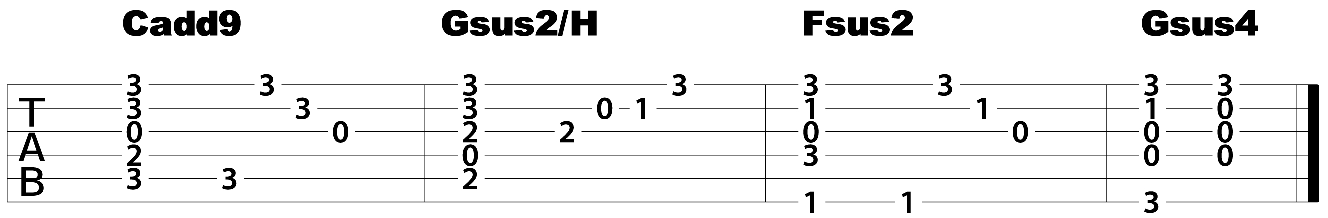
\includegraphics[width=345pt, height=60pt ]{res/jizvu.pdf}
\end{figure}
\leftskip 40pt
\rightskip 10pt
\hskip -50pt \begin{minipage}[t]{\textwidth} \chord{t}{x,p3,p5,p5,p3,p3}{Csus2} \end{minipage}
\hskip -15pt\begin{minipage}[t]{\textwidth}\chord{t}{p3,x,o,o,p1,p3}{Gsus4} \end{minipage}
\hskip -15pt\begin{minipage}[t]{\textwidth}\chord{t}{p3,x,o,o,o,p3}{G} \end{minipage}
\hskip -15pt\begin{minipage}[t]{\textwidth}\chord{t}{x,o,p2,o,p1,p3}{Ami7} \end{minipage}
\hskip -15pt\begin{minipage}[t]{\textwidth}\chord{t}{p1,x,p3,o,p1,p3}{Fsus2} \end{minipage}
\hskip -15pt\begin{minipage}[t]{\textwidth}\chord{t}{o,x,p2,o,p1,o}{C/E} \end{minipage}\\
}
}


\toftagthis{lucie}
\song{Medvídek}{Lucie}{80pt}{1}{
\verse{1}\A{}Dlouhá noc a mně se stýská moc,\\
pro tebe malý dárek mám.\\
Přes hory, \Hm{}přes ploty,\\
medvídek z \E[7]{}Bogoty už \A{}letí.  

\verse{2}Medvídek plyšový na cestě\\
křížový, Bůh ho ochrání\\
před smečkou \Hm{}římskejch psů\\
a jejich \E[7]{}úřadů\\
ti \D{}posílá lásku, co \E{}v bříšku má. 

\chorus{}\F{}Medvídek z Bogoty \A{}usnul a sní,\\
\F{}na kříži z Golgoty\A{} spí.\\
Za třicet \Hm{}stříbrných\\
z medvídka \E[7]{}padá sníh\\
no a ti \D{}římští psi\\
ho sjíždě\E{}jí na saních o Váno\A{}cích.
\clearpage
\leftskip 60pt
\verse{3}Nesvatá hodina medvídka proklíná,\\
že odhodil korunu bez trnů.\\
Medvídek ospalý pod křížem pokleká,\\
chce pít

\verse{4}Kalichem sladkosti medvídka\\
napustí do bříška, jak to má rád.\\
Koruna plyšová, vánoční cukroví,\\
nikdo se nedoví o svatozáři trnový.\\
\textbf{R:} 

\verse{*}\Am{}Medvídku, probuď se, \Am[/C]{}prober se, vstaň,\\
\Am[/F$\sharp$]{}psi se už \Am[/G]{}sbíhají, \Am[/E]{}připrav si dlaň,\\
slunce zas vychází, cítíš tu zář,\\
tlapky dáš v pěst, nebo nastavíš tvář. 

\Hm{}Římskejm psům a jejich \E{}úřadům\\
Maxipes \D{}Herodes vánoční \E{}slib dal dnes.\\
\textbf{R:}\\

}


\toftagthis{nohavica}
\song{Metro pro krtky}{Jaromír Nohavica}{70pt}{1}{
\verse{1}\G{}Prvá, druhá, \C{}třetí, \D{}čtvrtá,\G{} \hskip 1em \G{} \hskip 1em \C{} \hskip 1em \D{}\\
\G{}na za\G{}hradě \C{}krtek \D{}vrtá,\G{} \hskip 1em \G{} \hskip 1em \C{} \hskip 1em \D{}\\
\Em{} drápy \Em{}má jak \C{}výv\C{}rtky, oho\G{}ho,\\
\Am{} vrtá \Am{}metro \C{}pro krt\D{}ky, ohoho.\G{} \hskip 1em \G{} \hskip 1em \C{} \hskip 1em \D{}

\chorus{}Rrr ...

\verse{2}Každý, kdo si zaplatí, ohoho,\\
smí se projet po trati, ohoho,\\
od okurek po macešky, jé,\\
dál už musí každý pěšky, jé.

\chorus{}Rrr ...\\
}


\toftagthis{cechomor}
\song{Mezi horami}{Čechomor}{70pt}{1}{
\capo{5}
\verse{1}\revrpt{} \Em{}Mezi horami, lipka zelená, \rpt{}\\
\revrpt{} \G{}zabili Janka, \D{}Janíčka, \Em{}Janka\\
\Em{}miesto \D{}jele\Em{}ňa. \rpt{}

\verse{2}\revrpt{} Keď ho zabili, zamordovali, \rpt{}\\
\revrpt{}  na jeho hrobě, na jeho hrobě\\ 
kříž postavili. \rpt{}

\verse{3}\revrpt{} Ej, křížu, křížu, ukřižovaný, \rpt{}\\
\revrpt{}  zde leží Janík, Janíček, Janík\\ 
zamordovaný. \rpt{}

\verse{4}\revrpt{} Tu šla Anička plakat Janíčka, \rpt{}\\
\revrpt{}  hned na hrob padla a viac nevstala\\ 
dobrá Anička. \rpt{}\\
}

\toftagthis{nohavica}
\song{Mikymauz}{Jaromír Nohavica}{40pt}{0.9}{
\crdheight=2.3ex
\verse{1}\Am{}Ráno mě probouzí \G{}tma, sahám si na zápěs\F{}tí,\\
zda-li to \E{}ještě tluče, \Dm{}zda-li mám \E{}ještě štěstí,\\
\Am{}nebo je po mně a \G{}já mám voskované bo\F{}ty,\\
ráno co \E{}ráno stejné \Dm{}probuzení \E{}do nico\Am{}ty.

\vskip -2ex
\verse{2}Není co, není jak, není proč, není kam,\\
není s kým, není o čem, každý je v době sám,\\
vyzáblý Don Quijote sedlá svou Rosinantu\\
a Bůh je slepý řidič sedící u volantu.

\vskip -2ex
\chorus{}\E{}Zapínám \F{}telefon -- \Dm{}záznamník \E{}cizích citů,\\
špatné zprávy \F{}chodí jako \Dm{}policie, \E{}za úsvitu,\\
\Dm{}jsem napůl bdělý a \G[7]{}napůl ještě v noční pauze,\\
\C{}měl bych se smát, ale \E[sus4]{}mám ús\E{}měv Mikymauze,\\
\Am{}rána bych \Am[/G]{}zrušil. \hskip 1em \F{} \hskip 1em \E{} \hskip 1em \Am{}

\verse{3}Dobrý muž v rádiu pouští Čikoreu,\\
opravdu veselo je, asi jako v mauzoleu,\\
ve frontě na mumii mám kruhy pod očima,\\
růžový rozbřesk fakt už mě nedojímá.

\vskip -2ex
\verse{4}Povídáš něco o tom, co bychom dělat měli,\\
pomalu vychládají naše důlky na posteli,\\
všechno se halí v šeru, čí to bylo vinou,\\
že dřevorubec máchl mezi nás širočinou.

\leftskip 20pt
\chorus{}Postele rozdělené na dva suverénní státy,\\
ozdoby na tapetách jsou jak pohraniční dráty,\\
ve spánku nepřijde to, spánek je sladká mdloba,\\
že byla ve mně láska, je jenom pustá zloba,\\
dráty bych zrušil.

\verse{5}Prokletá hodina, ta minuta, ta krátká chvíle,\\
kdy věci nejsou černé, ale nejsou ani bílé,\\
kdy není tma, ale ještě ani vidno není,\\
bdění je bolest bez slastného umrtvení.

\vskip -2ex
\verse{6}Zběsile mi to tepe a tupě píchá v třísle,\\
usnout a nevzbudit se, nemuset na nic myslet,\\
opřený o kolena poslouchám tvoje slzy,\\
na život je už pozdě a na smrt ještě brzy.

\vskip -2ex
\chorus{}Co bylo kdysi včera, je, jako nebylo by,\\
káva je vypita a není žádná do zásoby,\\
věci, co nechceš, ať se stanou, ty se stejně stanou,\\
a chleba s máslem padá na zem vždycky blbou stranou,\\
máslo bych zrušil.

\verse{7}Povídáš o naději a slova se ti pletou,\\
jak špionážní družice letící nad planetou,\\
svlíknout se z pyžama, to by šlo ještě lehce,\\
dvacet let mluvil jsem a teď už se mi mluvit nechce.

\vskip -2ex
\verse{8}Z plakátu na záchodě prasátko vypasené\\
kyne mi, zatímco se kolem voda dolů žene,\\
všechno je vyřčeno a odnášeno do septiku,\\
jenom mně tady zbývá prodýchat pár okamžiků.

\vskip -2ex
\chorus{}Sahám si na zápěstí a venku už je zítra,\\
hodiny odbíjejí signály Dobrého jitra,\\
jsem napůl bdělý a napůl ještě v noční pauze,\\
měl bych se smát, ale mám úsměv Mikymauze,\\
\textls[-35]{rána bych zrušil\ldots{} lásku bych zrušil\ldots{} máslo bych zrušil.}\\
}


\toftagthis{filmove}
\song{Milenci v texaskách}{Starci na chmelu}{20pt}{1}{
\verse{1}\D{}Chodili spolu z čisté \Hm{}lásky \G{}a sedmnáct jim bylo \Hm{}let \hskip 1em \A[7]{}\\
\D{}a do té lásky bez nad\Hm{}sázky \G{}se vešel celý širý \Hm{}svět.\\
\G{}Ten svět v nich \Em{}ale viděl \Fsm{}pásky \G{}a jak by mohl nevi\A[7]{}dět,\\
\D{}vždyť horovali pro te\Hm{}xasky \G{}a sedmnáct jim bylo \Hm{}let.

\verse{2}A v jedné zvláště slabé chvíli, za noci silných úkladů,\\
ti dva se spolu oženili bez požehnání úřadů.\\
Ať vám to je či není milé, měla ho ráda, měl ji rád,\\
odpusťte dívce provinilé, jestli vám o to bude stát.

\verse{3}\D{}Ať vám to je či není \E[sus4/7]{}milé, \hskip 3em \G[maj]{} měla ho ráda, měl ji \H[sus2]{}rád\\
a bylo by moc pošetilé pro život hledat jízdní řád.\\
\textls[-9]{\G{}Tak jeden \Em[add9]{}mladík s jednou \Fsm{}slečnou \G{}se spolu octli na tra\A[7]{}ti,}\\
\D{}kéž dojedou až na ko\E[sus4/7]{}nečnou, \hskip 1em \G[maj]{}kéž na trati se nez\H[sus2]{}tratí,\\
\G[maj]{} kéž na trati se neztra\H[sus2]{}tí,\\
\G[maj]{} kéž na trati se neztra\H[sus2]{}tí\ldots{}
}


\toftagthis{nohavica}
\song{Milionář}{Jaromír Nohavica}{35pt}{0.9}{
U nás \D{}v domě říka\A[7]{}jí mi Franta \D{}Šiška,\D{}\\
bo už \D{}od pohledu \G{}chytrý jsem jak \D{}liška.\D{}\\
A když \D{}kery něco \Em{}neví nebo \A[7]{}když je na co \D{}levy,\\
tak jde \D{}za mnu a ja \A[7]{}všecko najdu \D{}v knižkach.\D{}\\
\D{} Ha \Em{}há, \hskip 0.5em \A[7]{}hahahá \D{}há,\\
tak jde \D{}za mnu a ja \A[7]{}všecko najdu \D{}v knižkach.\D{}

Raz mi říkal jeden známy dole v baře,\\
že s tu hlavu moh' bych do Milionaře.\\
Čemu ne, říkám si, brachu,\\
však má Železný dost prachu\\
no a Čechovi se podíváš do tváře.

Dostal jsem se mezi partu uchazeču.\\
Nikdo nemá šajnu jak tam nervy teču!\\
Všecko viděl jsem to hněde\\
tak jsem zmáčknul á, bé, cé, dé\\
no a už mě, kurva, ke stolečku vleču.

Čech to začal takým malým interiew,\\
co prý robim jestli kuřim a co piju.\\
Tak jsem řeknul, co jsem řeknul,\\
on se evidentně leknul\\
a už začly blikat světla ve studiu.\\

\leftskip -15pt
\large
\begin{minipage}[t]{0.54\textwidth}
\textls[-25]{První otázka, prý co je ukulele.\\
\textls[-55]{Tož to se přiznam měl jsem bobky u prdele.}\\
Tak jsem radši hlavu sklonil,\\
abych to všecko nezkonil,\\
říkám: \uv{Chtěl bych se obratit na přitele.}\\

Lojza byl po hlasu silně nevyspalý,\\
asi zase celu šichtu prochlastali.\\
Bylo slyšet, jak tam dycha,\\
ale třicet vteřin ticha.\\
To je tak, když se vam kamarád navali.\\

Moju staru zatím doma braly mory,\\
lidi ohryzávali televizory.\\
Tady nešlo nad čim plesat,\\
tož padesat na padesat,\\
ať vím, esi su to ty bulharské hory.\\

A už jasně na tym komputuře sviti:\\
buďto je to za A) vzácne lučni kviti,\\
nebo za B) nástroj strunny,\\
tu jde kurňa o koruny\\
a ja stejně jak na začátku jsem v řiti.\\

Čech tam zatím mával tymi svymi čisly.\\
Tak si řikam: Franta napij se a mysli.\\
Jake tudy sakypaky,\\
obratiš se na divaky,\\
však tu zatím za ty prachy enem kysli.}\\
\end{minipage}
\hskip 5pt
\begin{minipage}[t]{0.46 \textwidth}
\rightskip -25pt
\textls[-35]{Sám jsem byl zvědavý co publikum zvoli,\\
bo aj v obecenstvu možu sedět voli.\\
Devadesát procent za B),\\
ale to mi přišlo slabé,\\
bo co není stopro to mě dycky smoli.\\

Ještě že jsem chlap, co z boja neutika.\\
Říkám: \uv{Pane Čechu, pujdem do rizika.}\\
Měl jsem v gaťach nadělano,\\
ale Čech zakřičel: \uv{Ano,\\
máte pravdu, je to nástroj hudebnika!}\\
(Ha há, hahahá há, měl sem pravdu,\\
byl to nástroj hudebníka.)\\

Lidi tleskali, bo úspěch to byl plný.\\
Radosti zrobili dvě mexické vlny.\\
A já co mam srdce skromné,\\
jako všeci z Dolni Lomné,\\
jsem byl spokojený, bo sem ukol splnil.\\

\uv{\textls[-50]{Pane Čechu nerad přetáhnul bych strunu.}\\
Končim hru a beru tisicikorunu.}\\
Čech se jenom chytnul stolu,\\
obočí mu spadlo dolu\\
no a už se modry ku podlaze sunul.\\

První třidu do Ostravy Intercity.\\
V jidelňáku celu cestu valim kyty\\
a ta stovka co mi zbude,\\
to je přispěvek na chude,\\
bo Ostrava je region razovity.}
\end{minipage}
~\\
}

\toftagthis{nohavica}
\song{Milionář 2}{Jaromír Nohavica}{30pt}{1}{
\verse{1}Pane \D{}Nohavica, \A[7]{}znamý zpěva\D{}ku,\D{}\\
v živo\D{}tě jsem polknul \G{}křivdu kdeja\D{}ku,\D{}\\
ale \D{}to co vy jste \Em{}zrobil, tak to \A[7]{}jste mě fakt roz\D{}zlobil,\\
bo vy \D{}nemate cti \A[7]{}ani za ma\D{}ku.\D{}

\verse{2}Svévolně jste užil mého osudu,\\
zrobil jste ze mě hlupeho pobudu,\\
využil jste moji krize, jak jsem jel do televize,\\
v cele Dolní Lomné mám teď ostudu.

\verse{3}Stare baby, ba aj děcka nedospěle\\
po mně pokřikuji \uv{Franta ukulele!}\\
Zřekla se mě vlastní mama, musim chodit kanalama,\\
citim se jak sporťák Carda v TeleTele.

\verse{4}No a vy se zatím flákáte po TESCU,\\
mate velké auto, děcka, robu hezku,\\
za barakem modry bazen a ja stary cip a blázen\\
enem prazdnu kapsu a gatě na přezku.

\verse{5}Sto padesát tisíc prodaných cédeček,\\
tolik peněz, že se z toho chce až bečet,\\
natřískané kulturaky, baby ječí, chlapi taky,\\
no a za mnu se jen nouze s bídu vleče.

\verse{6}Napišu ten případ do krajského tisku,\\
že mě Nohavica okrad o část zisku,\\
buď se se mnou vyrovnáte, patřičný obnos mi dáte,\\
nebo dostanete u branky do pysku.

\verse{7}S úctou podepsany Franta Xaver Šiška,\\
sto osmdesát tři centimetrů výška,\\
boty dvanáct, vaha sto pět, jezdim v TIRu po Evropě\\
no a boxerky jsem dostal od Ježíška.\\
}


\toftagthis{zlutypes}
\song{Modrá}{Žlutý pes}{50pt}{1}{
\verse{1}\G{}Modrá je \D{}planeta, kde \C{}můžeme \D{}žít,\\
modrá je voda, kterou musíme pít,\\
modrá je obloha, když vodejde mrak,\\
modrá je \F{}dobrá, \C{}už je to \G{}tak.

\verse{2} Modrá je Milka -- ta naše kráva,\\
modrá je prej v Americe tráva,\\
modrá je údajně i polární liška,\\
senzačně modrá je moje vojenská knížka.

\chorus{}Jako \C{}nálada, když zahrajou poslední \G{}kus,\\
modrá je \F{}naděje, \C{}láska \F{}i moje \G{}blues.\\
Je to \C{}barva, kterou mám prostě \G{}rád,\\
modrá je \F{}dobrá, \C{}už je to \G{}tak.

\verse{3}Modrá je Raketa - ta moje holka,\\
modrá je vzpomínka na Mikyho Volka,\\
velká rána je modrej přeliv,\\
modrý voko má i černej šerif.\\
\textbf{R: $(2\times)$}

}

\toftagthis{folk}
\song{Montgomery}{Savana / tradicionál}{80pt}{0.94}{
\verse{1} \D{}Déšť ti, holka, smáčel \G{}vlasy, \Em{}\\
z \A[7]{}tvých očí zbyl prázdný \D{}kruh,\A[7]{}\\
kde je zbytek tvojí krásy,\\
to ví dneska jenom Bůh.

\chorus{}Z celé jižní eskadrony,\\
nezbyl ani jeden muž,\\
v Montgomery bijou zvony,\\
déšť ti smývá ze rtů růž.

\verse{2} Tam na kopci v prachu cesty,\\
leží i tvůj generál,\\
v ruce šátek od nevěsty,\\
ale ruka leží dál.\\
\textbf{R:}

\verse{3} Tvář má zšedivělou strachem,\\
zbylo v ní pár těžkých chvil,\\
proužek krve stéká prachem,\\
déšť mu slepil vlas jak jíl.\\
\textbf{R:}

\verse{4} Déšť ti šeptá jeho jméno,\\
šeptá ho i listoví,\\
lásku měl rád víc než život,\\
to ti nikdy nepoví.\\
\textbf{R:}\\
}


\toftagthis{kryl}
\song{Morituri te salutant}{Karel Kryl}{24pt}{0.87}{
\crdheight=2.3ex
\verse{1}Cesta je \Am{}prach a \G{}štěrk a \Dm{}udusaná \Am{}hlína\\
\C{}a šedé \F{}šmouhy \G[7]{}kreslí do vla\C{}sů\\
\revrpt{} a z hvězdných \F{}drah má \G{}šperk, co \C{}kamením se \E{}spíná,\\
\Am{}a pírka \G{}touhy z \Em{}křídel pega\Am{}sů. \rpt{}

\vskip -2ex
\verse{2}Cesta je bič, je zlá, jak pouliční dáma,\\
má v ruce štítky, v pase staniol\\
\revrpt{} a z očí chtíč jí plá, když háže do neznáma\\
dvě křehké snítky rudých gladiol. \rpt{}

\vskip -2ex
\chorus{}Seržante, \G{}písek je bílý, jak paže Daniely,\\
\Am{}počkejte chvíli, mé oči uviděly\\
\G[7]{}tu strašně dávnou vteřinu zapomnění,\\
\Am{}seržante, mávnou \G[7]{}a budem zasvěceni!\\
\C{}Morituri te salutant\E{}, morituri te salutant\ldots{}

\vskip -2ex
\verse{3}Tou cestou dál jsem šel, kde na zemi se zmítá\\
a písek víří křídla holubí\\
\revrpt{} a marš mi hrál zvuk děl, co uklidnění skýtá,\\
a zvedá chmýří, které zahubí. \rpt{}

\vskip -2ex
\verse{4}Cesta je tér a prach a udusaná hlína,\\
mosazná včelka od vlkodlaka,\\
\revrpt{} rezavý kvér -- můj brach a sto let stará špína\\
a děsně velká bíla oblaka. \rpt{}\\
\textbf{R:}
}



\toftagthis{anglicke}
\song{My Way}{Frank Sinatra}{30pt}{1}{
\capo{3}
\verse{1}And \G{}now, the end is \Hm[7/F$\sharp$]{}here,\\
and so I \Dm[6/F]{}face the final \E[7]{}curtain.\\
My \Am{}friend, I'll say it \Am[7/G]{}clear,\\
I'll state my \D[7/F$\sharp$]{}case of which I'm \G{}certain.\\
I've \G{}lived a life that's \G[7]{}full,\\
I traveled \C{}each and every \Cm{}highway\\
and \G{}more, much more than \D[7]{}this, I did it \Am[/G]{}my \hskip 2em \G{}way.

\verse{2}Regrets -- I've had a few,\\
but then again, too few to mention.\\
I did what I had to do\\
and saw it through without exemption.\\
I planned each charted course,\\
each careful step along the byway\\
and more, much more than this, I did it my way.

\chorus{}Yes, there were \G{}times, I'm sure you \G[7]{}knew,\\
when I bit \C{}off more than I could chew,\\
but through it \Am{}all, when there was \D[7]{}doubt,\\
I ate it \Hm{}up and spit it \Em{}out,\\
I faced it \Am{}all and I stood \D[7]{}tall and did it \Am[/G]{}my \hskip 2em \G{}way.

\verse{3}I've loved, I've laughed and cried,\\
I've had my fill, my share of losing.\\
And now, as tears subside,\\
I find it all so amusing.\\
To think I did all that\\
and may I say, not in a shy way,\\
\uv{Oh, no, oh, no, not me, I did it my way}

\chorus{}For what is a man, what has he got?\\
If not himself, then he has naught,\\
To say the things he truly feels\\
and not the words of one who kneels.\\
The record shows I took the blows and did it my way!
}




\toftagthis{brontosauri}
\song{Na kameni kámen}{Brontosauři}{40pt}{0.95}{
\verse{1}Jako \C{}suchej starej strom,\\
jako \F[maj]{}vše ničící hrom, jak v poli \C{}tráva,\C{}\\
připadá mi ten náš svět,\\
plnej \F[maj]{}řečí a čím \Am{}víc, tím \G{}líp se \C{}mám.\C{}

\chorus{}Budem \F[maj]{}o něco se rvát,\\
až tu \Am{}nezůstane \G{}stát na kameni \C{}kámen.\C{}\\
A jestli \F[maj]{}není žádnej Bůh,\\
tak nás \Am{}vezme země, vzduch, \G{}no a potom \C{}ámen.\C{}

\verse{2}A to všechno proto jen,\\
že pár pánů chce mít den bohatší králů.\\
Přes všechna slova, co z nich jdou,\\
hrabou pro kuličku svou, jen pro tu svou.\\
\textbf{R:}

\verse{3}Možná jen se mi to zdá\\
a po těžký noci přijde, přijde hezký ráno.\\
Jaký bude, nevím sám,\\
taky jsem si zvyk na všechno kolem nás.\\
\textbf{R:}\\
Na na ná na ná na ná\ldots
}


\toftagthis{hlas}
\song{Na kolena}{Ivan Hlas}{45pt}{1}{
\verse{1}Táhněte \C{}do háje, všichni \Am{}pryč,\\
chtěl jsem jít \C{}do ráje a nemám \Am{}klíč,\\
jak si tu \C{}můžete takhle \Am{}žrát,\\
ztratil jsem \F{}holku, co ji mám \G{}rád. 

\verse{2}Napravo, nalevo, nebudu mít klid,\\
dala mi najevo, že mě nechce mít,\\
zbitej a špinavej tancuju sám,\\
váš pohled káravej už dávno znám.\\
~\\
\chorus{}Pořád jen:\\
\revrpt{} \F{}na kolena, na kolena, \rpt{} \ \C{}jé jé jé, pořád jen\\
\revrpt{} \F{}na kolena, na kolena, \rpt{} \ \C{}jé jé jé, pořád jen\\
\revrpt{} \F{}na kolena, na kolena, \rpt{} \ \C{} je to \Am{}tak,\\
a vaše \F{}saka vám posere \G{}pták.\\
~\\
\verse{3}Cigáro do koutku si klidně dám,\\
tuhletu pochoutku vychutnám sám,\\
kašlu vám na bonton, vejmysly chytrejch hlav,\\
sere mě Tichej Don a ten váš tupej dav.\\
\textbf{R: }+ \ldots{}a tenhle barák vám posere pták.\\
}

\toftagthis{kabat}
\song{Na sever}{Kabát}{50pt}{0.85}{
\verse{1}\G{}No tak mi \Em{}zatancuj, ať \D{}náladu \G{}mám.\\
A dej mi celou noc, já nechci bejt sám,\\
hlavní je neuhnout, dobře zvolit svůj směr,\\
já teď, holka, musím jít až tam na sever.\\
\chorus{}\revrpt{} Cestu \G{}znám a \C{}neměním \G{}směr,\\
\G{}dojdu k ře\Em{}ce plný ryb až \D{}tam na se\G{}ver. \rpt{}

\verse{2} Procházím krajinou a lidi mě zvou,\\
čím těžší víno, lehčí holky tu jsou,\\
jedna z nich povídá -- dokud dávám, tak ber,\\
já ji jenom políbil a šel na sever.\\
\textbf{R:}

\verse{3} Mám nohy bolavý, už nechtěj' se hnout,\\
tou temnou vodou nechám tělo svý plout,\\
zakončím s noblesou ze všech poslední den,\\
kam mě vlny donesou, tam vsákne mě zem.\\
\textbf{R:}

\verse{*}Ta \D{}cesta byla rovná, místy rozbitá,\\
\C{}číše vína plná, jindy celá vylitá,\\
už \D{}nevrátím se zpátky, ubejvá mi sil,\\
tak \C{}řekněte jí, prosím, že \D{}jsem tady byl.

\chorus{}\textbf{\sffamily (A D A F$\sharp$mi E A)} 4$\times$
}


\toftagthis{buty}
\song{Nad stádem koní}{Buty}{18pt}{1}{
\verse{1}\D{}Nad stádem \textls[-35]{\A[sus4]{}}koní\hskip 0.3em - \hskip 0.3em \A{}í\hskip 0.6em \Em{} podkovy \G{}zvoní, zvoní,\\
černý vůz vlečou a slzy tečou a já volám,\\
\textls[-10]{tak neplač, můj kamaráde, náhoda je blbec, když krade.}\\
Je tuhý jak veka a řeka ho splaví, máme ho rádi,\\
no tak \C{}co, tak \G{}co, tak \A[sus4]{}co? \hskip 1.8em \A{}

\verse{2}Vždycky si přál, až bude popel, i s kytarou\\
vodou ať plavou, jen žádný hotel s křížkem nad hlavou.\\
Až najdeš místo, kde je ten pramen a kámen, co praská,\\
budeš mít jisto -- patří sem popel a každá láska,\\
no tak co, tak co, tak co?

\verse{3}Nad stádem koní podkovy zvoní, zvoní,\\
černý vůz vlečou a slzy tečou a já šeptám,\\
vysyp ten popel, kamaráde, do bílé vody, vody,\\
vyhasnul kotel a náhoda je štěstí od podko\G{}vy\D{}.\hskip 0.6em \G{} \hskip 0.7em \D{} \hskip 0.6em \G{}

\revrpt{}\G{} Vysyp ten \D{}popel, \A{}kamará\G{}de, \G{}do bílé \D{}vody, \A{}vo\G{}dy,\\
\G{}vyhasnul \D{}kotel a \A{}náhoda je\Em{} štěstí \Em{}od podko\G{}vy\D{}.\hskip 0.6em \G{} \hskip 0.7em \D{} \hskip 0.6em \G{} \rpt{} $^{3\times}$\\
}


\toftagthis{ceskekapely}
\song{Naděje}{Mezitím}{15pt}{1}{
\fontsize{13.6px}{2.8ex} \selectfont
\verse{1}\E{}Korálky z malin \H{}na krku nosí, \A{}ve vlasech předloňskej \E{}sníh.\\
\E{}Bez šatů a \H{}nožky má bosý, \A{}na ústech zvonivej \E{}smích.\\
\hskip -2.3ex \revrpt{} Chodí \A{}nahá a to jí nejvíc \E{}sluší, snídá \Csm{}déšť, pije z našich \A{}duší,\\
\E{}dává smích, \H{}tajný hřích, \A{}slzy smutku neosu\E{}ší. \rpt{}

\verse{2}Ze dlaní motýlům slaďounký nektar dá pít.\\
Písničkám do tónů zacinká ten její smích.\\
\hskip -2.2ex \revrpt{} Nemá hlas a přesto není němá, není dívka a není ani žena,\\
s tebou sní, už dvanáct dní je v tvojí mysli uvězněná. \rpt{}

\chorus{}\Csm{}Tajemná, tvý tajný \A{}přání sní \H{}zatímco ty \E{}spíš.\\
\Csm{}Tajemná, tak co ti \A{}brání jít \Fsm{}blíž a ještě \H{}blíž.\\
\Csm{}Tajemná, jak noční \A{}stíny, jak \H{}chorál z koste\E{}lů.\\
\Csm{}Tajemná, panenka z \A{}hlíny, s \E{}křídly andě\H{}lů.

\verse{3}Tajemství, až v žilách to mrazí, dá ti a nemůže víc.\\
Jak ti moc chybí, jak ti moc schází, měl bys jí konečně říct.\\
\hskip -2.4ex \textls[-28]{\revrpt{} Až ji potkáš a poznáš, že se chvěje, sklopí oči, kterýma se směje,}\\
jdi přímo k ní a řekni jí, že jsi bez ní bez naděje.\rpt{}\\
}

\toftagthis{plihal}
\song{Nagasaki, hirošima}{Karel Plíhal}{35pt}{1}{
\verse{1}\C{}Tramvají \G{}dvojkou \F{}jezdíval jsem \G{}do Žide\C{}nic\G{}, \hskip 0.8em \F{} \hskip 0.8em \G{}\\
\C{}z tak velký \G{}lásky\F{} většinou \G{}nezbyde nic\Am{}, \hskip 2em \Am{}\\
\F{}z takový \C{}lásky \F{}jsou kruhy \C{}pod očima\G{} \hskip 1em \G{}\\
a dvě \C{}spálený \G{}srdce -- \F{}Nagasaki, \G{}Hiroši\C{}ma.\G{} \hskip 0.8em \F{} \hskip 0.8em \G{}\\

\verse{2}Jsou jistý věci, co bych tesal do kamene,\\
tam, kde je láska, tam je všechno dovolené,\\
a tam, kde není, tam mě to nezajímá,\\
jó, dvě spálený srdce -- Nagasaki, Hirošima.

\verse{3}Já nejsem svatej, ani ty nejsi svatá,\\
ale jablka z ráje bejvala jedovatá,\\
jenže hezky jsi hřála, když mi někdy bylo zima,\\
jó, dvě spálený srdce -- Nagasaki, Hirošima.

\verse{4}Tramvají dvojkou jezdíval jsem do Židenic,\\
z tak velký lásky většinou nezbyde nic,\\
Z takový lásky jsou kruhy pod očima\\
a dvě spálený srdce -- Nagasaki, Hirošima.\\
a dvě \C{}spálený \G{}srdce -- \F{}Nagasaki, \G{}Hiroši\C{}ma,\G{}, \hskip 0.8em \F{} \hskip 0.8em \G{}\\
a dvě \C{}spálený \G{}srdce -- \F{}Nagasaki, \G{}Hiroši\C{}ma.
}


\toftagthis{ceskekapely}
\song{Nejlíp jim bylo}{Mňága a Žďorp}{20pt}{1}{
\capo{2}
\verse{1}
Nejlíp jim \C{}bylo\F[maj7]{}\\
\C{}když \F[maj7]{}nevěděli co dě\C{}lají\F[maj7]{} \hskip 3.2em \C{} \hskip 1em \F[maj7]{}\\
jenom se \G{}potkali 
\F{}a neznělo to \C{}špatně\F[maj7]{} \hskip 3.2em \C{} \hskip 1em \F[maj7]{}

Tak se snažili a opravdu si užívali,\\
jenom existovali a čas běžel skvěle.

\chorus{}
\F{}Nechám si projít \C{}hlavou
\G{}kam všechny věci \Am{}plavou,\\
\F{}jestli je všechno jen \C{}dech,
\G{}tak jako kdysi v noci\\
\Am{}spolu potmě na schodech\C{} \hskip 1em \F[maj7]{}

\verse{2}
Pak se ztratili
a chvílema se neviděli,\\
jenom si telefonovali
a byli na tom bledě.

A když se vrátili
už dávno nehořeli,\\
jenom dál usínali,
chvíli spolu, chvíli vedle sebe.\\
\textbf{R: $(3\times)$}\\
}


\toftagthis{ceskekapely}
\song{Nikdy nic nebylo}{Sto zvířat}{50pt}{1}{
\capo{3}
\verse{1}Nikdy jsi \Em{}nebyla a naše seznámení\\
proběhlo, \C{}má milá, před kinem, který není,\\
nepil jsem \Cs[dim]{}Tequilu a ne že bych se šklebil,\\
\D{}netlačil na pilu v tom baru, kterej nebyl.

\verse{2}Nikdy jsem neříkal, kolik mě čeká slávy,\\
nehrála muzika, ze který jsem se dávil,\\
nechtěl jsem na závěr Ti vyblejt celej život\\
a ztratit charakter a všechno oběživo.

\chorus{}\revrpt{} Nebylo \Em{}nic, já jen \G{}kdybys měla chvíli,\\
\A{}můžem si někam \Em{}sednout.\\
Nebylo nic, pár let jsme spolu nemluvili\\
a předtím taky ani jednou. \rpt{}

\verse{3}Nikdy nic nebylo, noc jako horská dráha,\\
vsadím se o kilo, že prostě nejsi drahá,\\
je to jen chiméra a žádný že jsem brečel\\
a měl jsem hysterák -- ty už mi neutečeš.

\verse{4}Scénář se nekoná, my dva ho nenapsali\\
a někdo místo nás prázdnej papír spálil,\\
\clearpage
nic není, ani já, ani tvý zlatý oči,\\
jen jsme šli na biják, co nikdo nenatočil\\
\textbf{R:}

\verse{5}Nikdy jsi nebyla a naše seznámení\\
proběhlo, má milá, před kinem, který není,\\
nic není, ani já, ani tvý zlatý oči,\\
jen jsme šli na biják co nikdo nenatočil.\\
\textbf{R:}\\
}



\toftagthis{anglicke}
\song{Nothing Else Matters}{Metallica}{70pt}{0.79}{
\vskip 5pt
\verse{1}So close, no matter how far,\\
couldn't be much more from the heart,\\
forever trustin' who we are\\
and nothing else matters.

\verse{2}Never opened myself this way,\\
life is ours, we live it our way,\\
all these words I don't just say\\
and nothing else matters.

\verse{3}Trust I seek and I find in you,\\
everyday for us something new,\\
open mind for a different view\\
and nothing else matters.

\chorus{}Never cared for what they do,\\
never cared for what they know\\
but I know.

\verse{4}So close\ldots{}\\
\textbf{R:} + \emph{acoustic solo}

\verse{5}Never opened\ldots{}

\verse{6}Trust I seek\ldots{} 

\chorus{}Never cared for what they say,\\
never cared for games they play,\\
never cared for what they do,\\
never cared for what they know,\\
and I know.\\
+ \emph{electric solo}

\verse{7}So close\ldots{}
}

\toftagthis{spiritual}
\song{Oh, Freedom}{americká lidová / Spirituál kvintet}{85pt}{1}{
\verse{1}\F{}Oh, Freedom, \C{}oh, \F{}Freedom,\Bb{} \hskip 1.2em \C{}\\
\F{}oh, \Dm{}Freedom, over me\G[7]{}. \hskip 1.5em \C{}\\
\chorus{}Be\A{}fore I'll be a \Dm{}slave,\\
I'd be \Bb{}buried in my \G[7]{}grave\\
and go \F{}home to my \C{}Lord\\
and be \Bb{}free!\F{}

\verse{2}No more weeping\ldots\\
\textbf{R:}\\
\verse{3}No more crying\ldots\\
\textbf{R:}\\
\verse{4}There'll be singing\ldots\\
\textbf{R:}

\verse{5}Jménem lásky, jménem hněvu\\
zpívám tobě, lide můj.

\chorus{}Nejvíc svobody si važ,\\
a čím víc ji postrádáš,\\
o to blíž v dobách zlých\\
při ní stůj!\\
}


\toftagthis{olympic}
\song{Okno mé lásky}{Olympic}{60pt}{0.9}{
\verse{1}\C{}Kdo tě líbá, když ne \F{}já,\\
\C{}kdo tě hlídá, když ne \F{}já,\\
\C{}okno v přízemí je \Bb{}zavřené i \F{}dnes, lásko \C{}má.

\verse{2}Kdo ti zpívá, když ne já,\\
kdo tě mívá, když ne já,\\
okno v přízemí je zavřené i dnes, lásko má. 

\chorus{}\Am{}A v jeho \G{}lesku vidím \F{}přicházet\\
\Am{}sebe ve \G{}věku patnáct \F{}let\\
\Am{}a znovu \G{}říkám spoustu \F{}něžných vět.\\
\C{}Ty, \F{}já, \C{}jsme \F{}my, \C{}my a \G{}náš je \F{}svět.

\verse{3}Kdo tě budí, když ne já,\\
kdo tě nudí, když ne já,\\
okno v přízemí je zavřené i dnes, lásko má.\\
\textbf{R:}

\verse{4}Kdo tě hladí, když ne já,\\
kdo tě svádí, když ne já,\\
kdo tě zradí, když ne já,\\
ty, já, jsme my, my a náš byl svět.\\
}

\toftagthis{filmove}
\song{Oliver twist}{Rebelové}{60pt}{0.8}{
\crdheight=2.2ex
\verse{1}\G{}Raději jsem neměla ten \Em{}román,\\
\Am{}raději jsem \D[7]{}neměla ho \G{}číst, \D[7]{}snad ani list.\\
\G{}Hrdina byl v tom románě \Em{}schován,\\
\Am{}miluji ho, \D[7]{}jmenuje se \G{}Twist, \C{}Oliver \G{}Twist.

\vskip -1.8ex
\chorus{}\Hm{}Takový muž na zemi už není,\\
jenom v knihách nebo dívčím snění,\\
\F{}přirovnám ho směle bez prodlení,\\
k \G{}to\F{}re\E{}rům, \G{}špa\F{}něls\E{}kým. \D[7]{}

\verse{2}Raději jsi neměla ten román,\\
raději jsi neměla ho číst, snad ani list.\\
Navždy měl tam zůstat v knize schován,\\
hrdina, co jmenuje se Twist, Oliver Twist.

\vskip -1.8ex
\chorus{}Namísto mne on ti ruší snění,\\
stále vzdycháš, proč jen živý není,\\
kdyby žil, tak dám se do učení\\
k torerům, španělským.\

\verse{3} Raději jsem neměla\dots

\verse{4}\Am{}Proč jsem se jen \D[7]{}naučila \G{}číst, \Em{}\\
\Am{}proč já blázen \D[7]{}dával ti to \G{}číst,\\
\Cs{}číst, \Bb{}ááá, \C{}ja-da-da-\G{}dam.
}

\toftagthis{olympic}
\song{Otázky}{Olympic}{40pt}{1}{
\verse{1}\C{}Kolik mám ještě dní, \F{}než přijde poslední,\\
\G{}jak dlouho budu zpívat a \C{}hrát.\\
Kolik je na zemi cest, kterou mám dát se vést,\\
nebo už myslet mám na návrat.

\chorus{}\C{}Posečkej, lásko \C[7]{}má, oka\F{}mžik,\\
\D[7]{}vždyť svět je veliký otaz\G{}ník.\\
\C{}Pořád se jenom ptáš \F{}a odpovědi, \G{}tý se nedoč\C{}káš.

\verse{*}\E{}Já jen vím, v zimě strom \Am{}ne \hskip 0.2em - \hskip 0.2em\Am[/G$\sharp$]{}kvete,\\
\Am[/G]{}v lé \hskip 0.4em - \hskip 0.4em \Am[/F$\sharp$]{}tě \hskip 0.4em sníh \hskip 0.2em \F{} nepadá, \E{}v noci je tma,\Am{}\\
\Am[/G$\sharp$]{}rád \hskip 0.4em tě \hskip 0.5em \Am[/G]{}mám, \hskip 0.6em \Am[/F$\sharp$]{}jen ne - \F{}ptej se \C{}proč, nevím \G{}sám.

\verse{2}Kde je tvůj dětský smích a proč je láska hřích,\\
kolik jen váží bolest člověčí.\\
Proč je zlato drahý kov\\ a proč je tolik prázdných slov,\\
proč chce každý být největší.\\
\textbf{R:}

\clearpage
\verse{*}Já jen vím, řeky proud hučí dál,\\
v žilách krev pěnivá, kdo ji tam dal,\\
rád tě mám, jen neptej se proč, nevím sám.

\verse{3}Kolik je slunci let, milión nebo pět,\\
myslíš, že zítra ráno vyjde zas.\\
Kolik je ulic, měst, proč umí kytky kvést,\\
proč nikdo neslyší můj hlas.
}


\toftagthis{ceskekapely}
\song{Otevřená zlomenina srdečního svalu}{Wanastowi Vjecy}{40pt}{0.96}{
\verse{1}Jsem jako \G{}vítr, kterej sfoukne pírko ze tvejch dlaní,\\
\D{}špínu jedný noci, jako hygiena ranní,\\
\Am{}velká voda slzí, který spláchnou noční hříchy,\\
\C{}tamburíny zvoní k \Eb{}operaci míchy.

Narovnám ti páteř, poškrábu ti záda,\\
pofoukám ti srdce, zrada kamaráda,\\
lásky účel světí prostředky a smetí,\\
špínu jedný noci, který neuletíš.

Otevřená zlomenina srdečního svalu,\\
trápení a kocovina, vůně tvýho žalu,\\
vypustíš svou hříšnou duši do slanýho moře,\\
neumírej, děvče moje, chci ti říct, že: 

\chorus{}Ohořelou \G{}károu chtěl bych dojet \D{}ke hvězdám,\\
který svítily z tvejch \Am{}očí, dřív než červo\C{}toči\\
se do tvýho srdce \F{}daj'.\D{}\\
V ohořelým autě už dva měsíce nedejchám,\\
sám se svojí vinou, už nikdy nechci jinou,\\
už asi nedoufám. 

\verse{2}Pláčem solíš otevřený rány, co se hojí,\\
tvoji krev i tělo příjímám pod obojí,\\
stejný lidi se soumrakem mají stejný stíny,\\
zmizelas jak před přízrakem, padám do hlubiny.

Tvůj pramínek vlasů zaliju včelím voskem,\\
koukám na tu krásu a nechápu to mozkem,\\
to, co jsi mi dala, já nikomu už nedám,\\
tak mi řekni, má opičko, proč tě marně hledám.

Otevřená zlomenina srdečního svalu,\\
trápení a kocovina, vůně tvýho žalu,\\
vypustíš svou hříšnou duši do slanýho moře,\\
neumírej, děvče moje, chci ti říct, že:\\
\textbf{R:}
}


\toftagthis{anglicke}
\song{Otherside}{Red Hot Chilli Peppers}{48pt}{1.1}{
\vskip 20pt

\chorus{}\Am{}How long, how \F{}long will I \C{}slide,\\
\G{}separate my \Am{}side,\hskip 0.5em \F{}\\
I \C{}don’t, I \G{}don’t believe it’s \Am{}bad,\hskip 0.5em \F{}\\
\C{}slittin' my throat, it’s \G{}all I ever\ldots

\verse{1}\Am{}I heard your voice through a \Em{}photograph,\\
\Am{}I thought it up it brought \Em{}up the past,\\
\Am{}once you know you can \Em{}never go back,\\
I’ve got to \G{}take it on the \Am{}otherside.

\verse{2}Centuries are what it meant to me,\\
a cemetery where I marry the sea,\\
stranger things could never change my mind,\\
I’ve got to take it on the otherside,\\
\G{}take it on the \Am{}otherside,\\
\G{}take it on, \Am{}take it on.\\
\textbf{R:}

\clearpage
\verse{3}Pour my life into a paper cup,\\
the ashtray’s full and I’m spilling my guts,\\
she wants to know am I still a slut,\\
I’ve got to take it on the otherside.

\verse{4}Scarlet starlet and she’s in my bed,\\
a candidate for my soul mate bled,\\
push the trigger and pull the thread,\\
I’ve got to take it on the otherside,\\
take it on the otherside,\\
take it on, take it on.\\
\textbf{R: $(2\times)$}
}

\toftagthis{krestan}
\song{Panenka}{Robert Křesťan}{70pt}{1}{
\verse{1}Co \D{}skrýváš za \G{}víčky a \D{}plameny \G{}svíčky,\\
snad \D{}houf bílých holubic nebo jen \A{}žal?\\
Tak \G{}odplul ten \D{}prvý den, \G{}zmáčený \D{}krví,\\
ani pouťovou panenku \A[7]{}nezane\D{}chal.

\chorus{}Otevři \G{}oči, ty \D{}uspěcha\A{}ná,\\
\G{}dámo \D{}uplaka\A{}ná,\\
\G{}otevři \D{}oči, ta \G{}hloupá noc \D{}končí,\\
a mír je \A[7]{}mezi ná\D{}ma.

\verse{2}Už si oblékni šaty i řetízek zlatý\\
a umyj se, půjdeme na karneval.\\
A na bílou kůži ti napíšu tuší,\\
že dámou jsi byla a zůstáváš dál.\\
\textbf{R:}\\
}


\toftagthis{anglicke}
\song{Perfect Day}{Lou Reed}{40pt}{1}{
\E{} \hskip 1em \Am{} \hskip 2em \E{} \hskip 1em \Am{}\\
\verse{1}\Am{}Just a \D{}perfect day,\G{} drink sangria \C{}in the park,\\
\F{}then later when \Dm{}it gets dark we go\E{} home.

\verse{2}Just a perfect day, feed animals in the zoo,\\
then later a movie, too, and then home.

\chorus{}Oh, \A{}it's such a \D{}perfect day,\\
\Csm{}I'm glad I spent it with \D{}you.\\
\A{}Oh, such a \E{}perfect day,\\
\revrpt{} you just \Fsm{}keep me \E{}hanging \D{}on, \rpt{}

\verse{3}Just a perfect day, problems all left alone,\\
weekenders on our own, it's such fun.

\verse{4}Just a perfect day, you made me forget myself,\\
I thought I was someone else, someone good.\\
\textbf{R:}

\revrpt{} \Csm{}You're gonna \G{}reap just what you \D{}sow.\A{} \hskip 1em \rpt{}\\
}


\toftagthis{nohavica}
\song{Petěrburg}{Jaromír Nohavica}{12pt}{0.92}{
\textls[-20]{\verse{1}\Am{}Když se snáší noc na střechy Petěrburgu, \F{}padá \E{}na mě \Am{}žal,\\
\textls[-35]{zatoulaný pes nevzal si ani kůrku \F{}chleba, kterou \E{}jsem mu \Am{}dal.}

\chorus{}\revrpt{} \C{}Lásku moji \Dm{}kníže I\E{}gor si bere,\\
\F{}nad sklenkou \Ds[dim]{}vodky \hskip 0.5em \H[7]{}hraju si \E{}s revolverem,\\
\Am{}havran usedá na střechy Petěrburgu, \F{}čert a\E{}by to \Am{}spral. \rpt{}

\textsl{Mezihra (akordy sloka + 2$\times$ ref.)} 

\verse{2}Nad obzorem letí ptáci slepí v záři červánků,\\
moje duše, široširá stepi, máš na kahánku.

\chorus{}\revrpt{} Mému žalu na světě není rovno,\\
vy jste tím vinna, Naděždo Ivanovno,\\
vy jste tím vinna, až mě zítra najdou s dírou ve spánku. \rpt{}\\}
\noexport{
~\\
\hskip -17pt \textbf{\large Mezihra:}
\vskip -2pt

\begin{figure}[h]
\leftskip -5pt
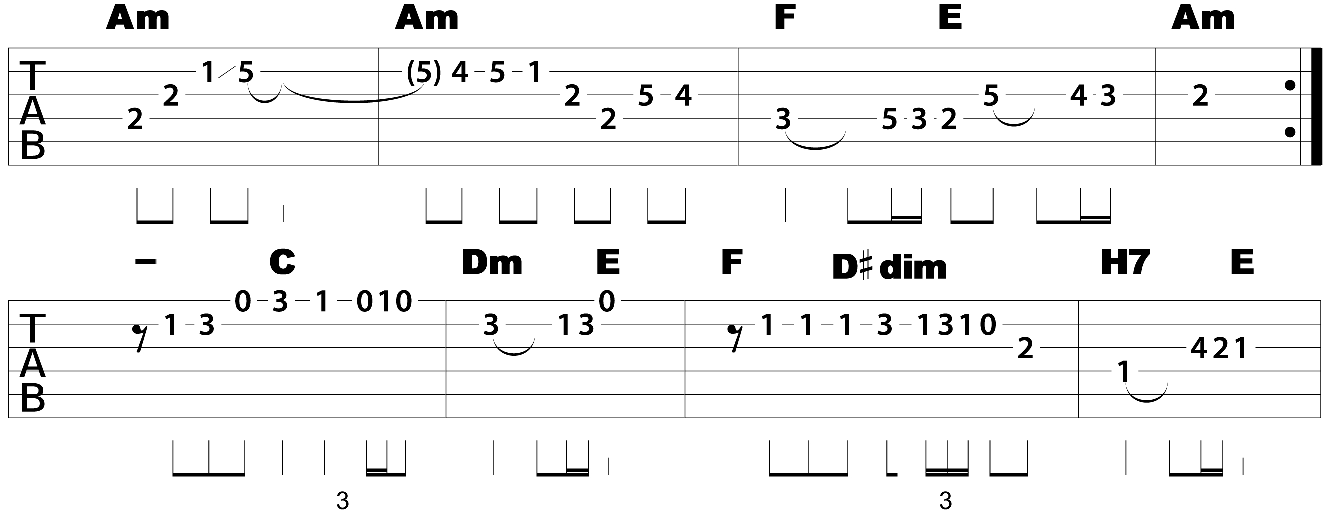
\includegraphics[width=370pt, height=133pt]{res/peterburg.pdf}
\vskip -15pt
\end{figure}
}
}

\toftagthis{nohavica}
\song{Pijte vodu}{Jaromír Nohavica}{65pt}{0.88}{
\chorus{}\revrpt{} \C{}Pijte vodu, pijte pitnou vodu,\\
pijte vodu a \G[7]{}nepijte \C{}rum. \rpt{}

\vskip -1ex
\verse{1}Jeden smutný ajznboňák\\
pil na pátém nástupišti Air Cognac.\\
Huba se mu slepila,\\
diesel lokomotiva ho zabila.\\
\textbf{R:}

\vskip -1.5ex
\verse{2} V rodině u Becherů\\
pijou becherovku přímo ze džberů.\\
Proto všichni Becheři\\
mají trable s játrama a páteří.\\
\textbf{R:}

\vskip -1.5ex
\verse{3}Pil som vodku značky Gorbatschow\\
a potom povedal som všeličo a volačo.\\
Vyfásol som za to tri roky,\\
teraz pijem chlorované patoky.\\
\textbf{R:}

\vskip -1.5ex
\verse{4}Jesteśmy chłopci z Warszawy,\\
jeżdżimy pociągiem za robotą do Ostrawy.\\
Cztery litry wódki a mnóstwo piw,\\
po prostu bardzo fajny kolektyw.\\
\textbf{R:}

\vskip -1.5ex
\verse{5}Jedna paní v Americe\\
ztrapnila se převelice.\\
Vypila na ex rum\\
a poblila jim Bílý dům.\\
\textbf{R:}\\
}


\toftagthis{sverakuhlir}
\song{Píseň proti trudomyslnosti}{J. Uhlíř / Z. Svěrák}{13pt}{1}{
\textls[-10]{\D{}Polární noc má zvláštní moc, každého přepadne smu\A[7]{}tek,\\
Němec i Brit, křesťan i Žid, každý by nejradši ute\D{}k',\\
ba i ti \G{}šikovní Žapon\D{}ci se sila\E[7]{}mi jsou na kon\A[7]{}ci,\\
jen jeden z \D{}národů nesko\G{}ná, hrůzy seve\D{}ru slavně \A[7]{}překo\D{}ná!\\}
~\\
Tam, kde hy-, tam, kde hy-, tam, kde hynou vl\A[7]{}ci,\\
tam, kde hy-, tam, kde hy-, tam kde hynou vl\D{}ci,\\
tam, kde hy-, tam, kde hy-, tam kde hynou so\G{}bi,\\
\A[7]{}Čech se přizpůso\D{}bí! \A[7]{}Čech se přizpůso\D{}bí!\A[7]{}\hskip 1.8em \D{}\\
}


\toftagthis{slovenske}
\song{Po schodoch}{Richard Müller}{35pt}{1}{
\verse{1}\Am{}Výťah opäť nechodí, tak \G{}zdolať 13 poschodí\\
\F{}zostáva mi \G{}znova po svo\Am{}jich.\\
Na schodoch čosi šramotí a neón kde tu nesvieti,\\
ešte že sa po tme nebojím.

\verse{2}Počuť hlasné stereo aj výstrahy pred neverou\\
ktosi čosi vŕta v paneloch.\\
Tatramatky ródeo zas mieša sa tu s operou,\\
\F{}všetko počuť \G{}cestou po scho\Am{}doch.\Em{}

\chorus{}\revrpt{} Cestou \Am{}po schodoch, \Em{}po schodoch,\\
\F{}poznávam \G{}poschodia,\\
poznám \Am{}po schodoch, \Em{}po zvukoch,\\
\F{}čo sme kto \Em{}za ľu\Am{}dia. \rpt{}

\verse{3}Štekot smutnej kólie, za premárnené prémie\\
vyhráža sa manžel rozvodom.\\
Disko, tenis, árie, kritika televízie,\\
oddnes chodím iba po schodoch.\\
\textbf{R:}
}


\toftagthis{nedvedi}
\song{Podvod}{Jan Nedvěd}{15pt}{0.9}{
\capo{2}
\verse{1}\Em{}Na dlani jednou z tvých řas, do tmy se \Am{}koukám,\\
\D{}hraju si písničky tvý, co sem ti \G{}psal.\\
Je skoro \Am{}půlnoc a z kostela \Am[/C]{}zvon mi noc připo\Em{}míná,\\
půjdu se \Am{}mejt a pozhasí\Am[/C]{}nám, co bude \H[7]{}dál?

\verse{2}Pod polštář dopisů pár, co poslalas dávám,\\
píšeš, že ráda mě máš a trápí tě stesk.\\
Je skoro půlnoc a z kostela zvon mi noc připomíná,\\
půjdu se mejt a pozhasínám, co bude dál?

\chorus{}Chtěl jsem to \Am{}ráno, kdy naposled snídal jsem s tebou,\\
ti \Em{}říct, že už ti nezavolám,\\
pro jednou pitomou \Am{}holku, pro pár noci \D{}touhy,\\
podved' jsem \G{}všechno, o čem doma si \H[7]{}sníš,\\
teď je mi to \Em{}líto.

\verse{3}Kolikrát člověk může mít rád tak opravdu z lásky,\\
dvakrát či třikrát -- to ne, i jednou je dost.\\
Je skoro půlnoc a z kostela zvon mi noc připomíná,\\
půjdu se mejt a pozhasínám, co bude dál?\\
\textbf{R: ($2\times$)}
}


\toftagthis{kabat}
\song{Pohoda}{Kabát}{80pt}{1}{
\vskip 8pt
\CHORD{\revrpt{}}{} \hskip 0.7em \D{} \hskip 1em \A{} \hskip 1em \E{} \hskip 1em \Hm{} \hskip 2em \CHORD{\rpt}{}\\
\verse{1}\Fsm{} Vezmu tě, má milá, \Csm{}rovnou k nám,\\
\Fsm{} kolem louky, lesy, \Csm{}hejna vran,\\
\Fsm{} všude samá \E{}kráva, samej \Hm{}vůl.

\verse{2}Máme kino, máme hospodu,\\
v obci všeobecnou pohodu,\\
máme hujer, žito, chléb i sůl.

\chorus{}\D{}Když se u nás chlapi \A{}poperou,\\
tak jenom \E{}nožem anebo \Hm{}sekerou,\\
v zimě tam \D{}dlouhý noci \A{}jsou\\
a tuhej \Hm{}mráz.\Hm{}\\
Jak jsou naše cesty zavátý,\\
tak vezmem vidle anebo lopaty,\\
když něco nejde, co na tom sejde,\\
my máme čas.

\verse{3}Chlapi někdy trochu prudký jsou,\\
holky s motykama tancujou,\\
s ranní rosou táhnou do polí.

\clearpage
\verse{4} Nikdo se tam nikam nežene,\\
máme traktory a ne, že ne,\\
až to spatříš, ledy povolí.\\
\textbf{R:}

\verse{5}Hoří les a hoří rodnej dům,\\
hoří velkostatek sousedům,\\
to je smůla, drahá, podívej.

\verse{6}Hasiči to stejně přejedou,\\
oni si moc dobře nevedou,\\
schovej sirky, ať je neviděj.\\
\textbf{R: ($2\times$)}
}


\toftagthis{nohavica}
\song{Pochod marodů}{Jaromír Nohavica}{30pt}{1}{
\verse{1}\Dm{}Krabička cigaret a \F{}do kafe \C{}rum, \Bb{}rum, \Dm{}rum,\\
dvě vodky a fernet a teď, \F{}doktore, \C{}čum, \Bb{}čum, \Dm{}čum,\\
chra\Gm{}pot v hrud\Bb{}ním ko\Dm{}ši, no \Gm{}to je \Bb{}záži\A{}tek,\\
\Dm{}my jsme kámoši řidi\F{}čů sani\C{}tek, -\Bb{}tek, -\Dm{}tek.

\verse{2}Měli jsme ledviny, ale už jsou nadranc, -dranc, -dranc,\\
i tělní dutiny už ztratily glanc, glanc, glanc,\\
u srdce divný zvuk, co je to, nemám šajn,\\
je to vlastně fuk, žijem fajn, žijem fajn, fajn, fajn.

\chorus{}\Dm{}Cirhóza, \F{}trombóza, \C{}dávivý \F{}kašel,\\
\Gm{}tuberku\Dm{}lóza -- \A{}jó, to je \Dm{}naše!\\
Neuróza, \F{}skleróza, \C{}ohnutá \F{}záda,\\
\Gm{}paraden\Dm{}tóza, no \A{}to je pa\Dm{}ráda!\\
Jsme \Gm{}slabí na tě\Dm{}le, ale \C{}silní na du\F{}chu,\\
\Gm{}žijem vese\Dm{}le, \hskip 1em \A{}juchuchuchu\Dm{}chu!

\verse{3}Už kolem nás chodí pepka mrtvice, -ce, -ce,\\
tak pozor, marodi, je zlá velice, -ce, -ce,\\
zná naše adresy a je to čiperka,\\
koho chce, najde si, ten natáhne perka, -rka, -rka.

%\leftskip 50pt
\verse{4}Zítra nás odvezou, bude veselo, -lo, -lo,\\
doktoři vylezou na naše tělo, -lo, -lo,\\
budou nám řezati ty naše vnitřnosti\\
a přitom zpívati ze samé radosti, -sti, -sti.

\chorus{}Zpívati: \Dm{}Cirhóza, \F{}trombóza, \C{}dávivý \F{}kašel,\\
\Gm{}tuberku\Dm{}lóza, hele, \A{}já jsem to \Dm{}našel!\\
Neuróza, \F{}skleróza, \C{}křivičná \F{}záda,\\
\Gm{}paraden\Dm{}tóza, no \A{}to je pa\Dm{}ráda!\\
Byli \Gm{}slabí na tě\Dm{}le, ale \C{}silní na du\F{}chu,\\
\Gm{}žili vese\Dm{}le, než \A{}měli poru\D{}chu!\\
}


\toftagthis{nohavica}
\song{Potulní kejklíři}{Jaromír Nohavica}{40pt}{0.8}{
\verse{1}\Am{} Potulní kejklíři \Em{}jdou zasněženou plá\Am{}ní, \hskip 1em \Em{}\\
\Am{} v obitém talíři \Em{}vaří vítr ke snída\Am{}ni. \hskip 1em \Em{}\\
\C{} S cvičenou opičkou \G{}na rameni,\\
\Am{}životem\Dm{} malin\G{}ko \C{}unave\E[7]{}ni,\\
\Am{}potulní kejklíři \Em{}jdou bílou plá\Am{}ní. \hskip 1em \Em{}

\verse{2}V kovárně na kraji vsi všechen sníh už ztál,\\
dobrý kovář odžene psy a pozve je dál,\\
sláma je postelí i peřinou\\
a oni jeden k druhému se přivinou\\
a zítra na návsi začíná candrbál.

\chorus{}\revrpt{} \Am{}Kejklíři, \Em{}kejklíři \Am{}jdou\ldots{}\Em{} \hskip 1.5em \rpt{} 

\verse{3}Po schodech kostela poskakuje míč,\\
muž s tváří anděla ohýbá železnou tyč.\\
A krásná dívka jménem Marína\\
zatančí tanec pohanského bůžka Odina\\
a zítra po polednách budou zase pryč.\\
\textbf{R:}

\verse{4}Vozíček z lipových dřev po hlíně drkotá,\\
červená nepokojná krev je erbem života,\\
všechno, co chceme, leží před námi\\
za devatero poli, devatero řekami,\\
nad zimní krajinou slunce blikotá.\\
\textbf{R: $(2\times)$}\\
}


\toftagthis{folk}
\song{Pověste ho vejš}{Michal Tučný}{45pt}{0.9}{
\rec{\emph{\Em{}}Na dnešek jsem měl divnej sen,\\
slunce pálilo a před salonem\\
stál v prachu dav, v tvářích cejch očekávání,\\
uprostřed šibenice z hrubých klád.\\
Šerifův pomocník sejmul z hlavy odsouzenci kápi\\
a dav zašuměl překvapením.\\
I já jsem zašuměl překvapením.\\
Ten odsouzenec jsem byl já\\
a šerif četl neúprosným hlasem rozsudek:}

\chorus{}Pověste ho \Em{}vejš, ať se houpá,\\
pověste ho \G{}vejš, ať má \D{}dost.\\
Pověste ho \Am{}vejš, ať se \Em{}houpá,\\
že tu \D{}byl nezvanej \Em{}host.

\verse{1} Pověste ho, že byl jinej,\\
že tu s náma dejchal stejnej vzduch.\\
Pověste ho, že byl línej\\
a tak trochu dobrodruh.

\verse{2}Pověste ho za El Passo,\\
za snídani v trávě a lodní zvon.\\
Za to, že neoplýval krásou,\\
že měl \C{}country rád a že se \H[7]{}uměl smát i \Em{}vám.

\verse{*}Nad hla\G{}vou mi slunce \D{}pálí,\\
konec \Am{}můj nic neod\G{}dá\D{}lí.\\
Do svých \G{}snů se dívám \D{}zdáli,\\
a \Am{}do uší mi stále zní tahle \H[7]{}moje píseň poslední.

\verse{3} Pověste ho za tu banku,\\
v který zruinoval svůj vklad.\\
Za to, že nikdy nevydržel\\
na jednom místě stát.

\verse{*} Nad hlavou\ldots{}\\
\textbf{R:}

\verse{4} Pověste ho za tu jistou,\\
který nesplnil svůj slib,\\
že byl zarputilým optimistou\\
a tak dělal spoustu chyb.

\verse{5} Pověste ho, že se koukal,\\
že hodně jed' a hodně pil,\\
že dal přednost jarním loukám\\
a pak se \C{}oženil a pak se \H[7]{}usadil a \Em{}žil.\\
\textbf{R: $(2\times)$}
}

\toftagthis{suchyslitr}
\song{Pramínek vlasů}{Jiří Suchý}{50pt}{0.95}{
\verse{1}Když měsíc \C{}rozlije\Am{} světlo své \F[6]{}po kraji\G[6]{}\\
a hvězdy řeknou, že čas je jít spát,\\
pramínek vlasů jí ustřihnu potají,\\
komu --  no \C{}přece té,\F[7]{} kterou mám \C{}rád.\G[7]{}

\verse{2}Pramínek vlasů jí ustřihnu potají,\\
já blázen pod polštář chci si ho dát.\\
Ačkoliv sny se mi zásadně nezdají,\\
věřím, že dnes v noci budou se zdát.

\chorus{}O sny mě \Bb{}připraví teprve \C{}svítání,\\
zpěv ptáků v \Bb{}oblacích a modré \C{}nebe.\\
Od vlasů, \F{}jichž jsem se dotýkal \C{}ve spaní,\\
nový den \Ab[7]{}nůžkama odstřihne \G{}tebe.

\verse{3}A na bílém polštáři, do kroužku stočený,\\
zbude tu po tobě pramínek vlasů.\\
Já nebudu vstávat, dál chci ležet zasněný,\\
je totiž neděle a mám dost času.\\
\textbf{R:}

\verse{4}A na bílém polštáři\dots\\
\revrpt{}\ldots{}je totiž neděle a mám dost času. \rpt{}\\
}



\toftagthis{ceskekapely}
\song{Proklínám}{Janek Ledecký}{20pt}{1}{
\verse{1}
Prázdnej \Am{}byt je jako \F{}past, 
kde \Dm{}růže uvad\C{}nou. \G{}\\
\Am{}Potisící\F{} čtu tvůj dopis \Dm{}na rozlouče\G{}nou.\\\
\C{}Píšeš že \Am{}odcházíš, když \F{}den se s nocí \C{}stří\G{}dá.\\
\Am{}Vodu z vína\F{} udělá, kdo \Dm{}dobře nehlí\G{}dá. Píšeš:

\chorus{}\C{}Proklíná\G{}m,\hskip 0.3em \Am{} ty tvoje \F{}ústa, proklíná\C{}m\\
tvoje \G{}oči ledo\Am{}vý,
v \F{}srdci jen sníh,\C{} sám a sá\G{}m.\\
\Am{}Ať nikdy \F{}úsvit nespatř\C{}íš,
na ústa mř\G{}íž,  oči oslep\Am{}nou.\\
Ať \F{}do smrti seš s\C{}ám.

\verse{2}Tvoje oči jsou jak stín a tvář -- den, když se stmívá.\\
Stromy rostou čím dál výš a pak je čeká pád.\\
Sám s hlavou skloněnou,všechny lásky budou zdání.\\
Potisící čtu tvůj dopis na rozloučenou. Píšeš:\\
\textbf{R:} \dots ať \F{}do smrti seš s\C{}ám a sá\G{}m.\\
Ať nikdy úsvit nespatříš\dots\\
}


\toftagthis{cechomor}
\song{Proměny}{Čechomor}{50pt}{1}{
\verse{1}\Am{}Darmo sa ty trápíš, \G{}můj milý sy\C{}nečku,\\
nenosím já tebe, \E[7]{}nenosím v sr\Am{}déčku,\\
přece tvo\G{}ja \C{}ne - \G{}bu - \C{}du, \Dm{}ani jednu \E{}hodi\Am{}nu.

\verse{2}Copak sobě myslíš, má milá panenko,\\
vždyť ty jsi to moje rozmilé srdénko\\
a ty musíš býti má, lebo mi tě Pán Bůh dá.

\verse{3}A já sa udělám malú veveričkú\\
a já ti uskočím z dubu na jedličku,\\
přece tvoja nebudu, ani jednu hodinu.

\verse{4}A já chovám doma takú sekérečku,\\
ona mi podetne dúbek i jedličku\\
a ty musíš býti má, lebo mi tě Pán Bůh dá.

\verse{5}A já sa udělám tú malú rybičkú\\
a já ti uplynu preč po Dunajíčku,\\
přece tvoja nebudu, ani jednu hodinu.

\verse{6}A já chovám doma takovú udičku,\\
co na ni ulovím kdejakú rybičku\\
a ty přece budeš má, lebo mi tě Pán Bůh dá.

\optVerse{-30pt}{20pt}{-15pt}{
\emph{housle}\ \ \revrpt{} \textbf{\sffamily Ami \ Ami \ F \ C \ F \ C \ G \ G} \rpt
}

\verse{7}A já sa udělám tú velikú vranú\\
a já ti uletím na Uherskú stranu,\\
přece tvoja nebudu, ani jednu hodinu.

\verse{8}A já chovám doma starodávnú kušu,\\
co ona vystřelí všeckým vranám dušu\\
a ty musíš býti má, lebo mi tě Pán Bůh dá.

\verse{9}A já sa udělám hvězdičkú na nebi\\
a já budu lidem svítiti na nebi,\\
přece tvoja nebudu, ani jednu hodinu.

\hskip -8pt\verse{10}A sú u nás doma takoví hvězdáři,\\
co vypočítajú hvězdičky na nebi\\
\revrpt{} a ty musíš býti má, lebo mi tě Pán Bůh dá. \rpt{}

\optVerse{-30pt}{20pt}{-15pt}{
\emph{housle}\ \ \revrpt{} \textbf{\sffamily Ami \ Ami \ F \ C \ F \ C \ G \ G} \rpt
}
}


\toftagthis{chinaski}
\song{První signální}{Chinaski}{35pt}{1}{
\verse{1}Až si \G{}zejtra ráno \C{}řeknu zase \Em{}jednou provždy dost,\\
\G{}právem se mi \C{}budeš tiše \Em{}smát.\\
Jak omluvit si svoji slabost, nenávist a zlost,\\
když za všechno si můžu vlastně sám.

\chorus{}Za \Am{}spoustu dní, možná za \C{}spoustu let,\\
až se mi \G{}rozední, budu ti \D{}vyprávět\\
na první signální, jak jsem vobletěl svět,\\
jak tě to vomámí a nepustí zpět.\\
Jaký si to \F{}uděláš, \Bb{}takový to \Dm{}máš.\\
Jaký si to \F{}uděláš, \Bb{}takový to \Dm{}máš.

\verse{2}Až se dneska večer budu tvářit zas jak Karel Gott,\\
budu zpívat vampam tydam pam.\\
Všechna sláva, polní tráva, ale peníz přijde vhod,\\
jak jsem si to udělal, tak to mám.

\chorus{}Za spoustu dní \dots{}\\
\dots jak tě to vomámí a nepustí zpět.\\
Ná nana \Am{}ná naná, ná nana \C{}ná naná \dots

\revrpt{} Jaký si to uděláš, takový to máš. \rpt{}\\
}


\toftagthis{nohavica}
\song{Přítel}{Jaromír Nohavica}{30pt}{0.9}{
\vskip -5pt
\capo{2}
\crdheight=2.2ex
\verse{1}Jestlipak \G{}vzpomínáš si ještě na ten \D[/F$\sharp$]{}čas,\\
táhlo nám \Am[7/E]{}na dvacet a slunko bylo v \D{}nás,\\
\Am{}vrabci nám jedli z ruky, \C{}život šel bez záruky,\\
\G{} ale taky bez pří\D[/F$\sharp$]{}kras.

\verse{2}Možná, že hloupý, ale krásný byl náš svět,\\
zdál se nám opojný jak dvacka cigaret\\
a všechna tajná přání plnila se na počkání\\
anebo rovnou hned.

\chorus{}\Am{}Kam jsme se poděli, \C{}kam jsme se to poděli,\\
\G{}kde je ti \D[/F$\sharp$]{}konec, m\Em[7]{}ůj jediný příteli,\\
\Am{}zmizels mi, nevím \D{}kam,\\
\C[add9]{}sám, sám, sám, jsem tady \G{}sám.\D[/F$\sharp$]{} \hskip 2.5em \Am[7/E]{} \hskip 3.7em \D{}

\verse{3}Jestlipak vzpomínáš si ještě na tu noc,\\
jich bylo pět a tys mi přišel na pomoc,\\
jó, tehdy nebýt tebe, tak z mých dvanácti žeber\\
nezůstalo příliš moc.

\verse{4}Dneska už nevím, jestli přiběh' by jsi zas,\\
jak tě tak slyším, máš už trochu vyšší hlas,\\
a vlasy, vlasy kratší, jó, bývali jsme mladší,\\
no a co, vem to ďas.

\chorus{}Kam jsme se poděli, kam jsme se to poděli,\\
kde je ti konec, můj jediný příteli,\\
zmizels mi, nevím kam,\\
sám, sám, sám, peru se teď sám.

\verse{5}Jestlipak vzpomínáš si ještě na ten rok,\\
každá naše píseň měla nejmíň třicet slok\\
a my dva jako jeden ze starých reprobeden\\
přes moře jak přes potok.

\verse{6}Tvůj děda říkal: \uv{Ono se to uklidní,}\\
měl pravdu, přišla potom spousta malých dní\\
a byla velká voda, vzala nám, co jí kdo dal,\\
a tobě i to poslední.

\chorus{}Kam jsme se poděli, kam jsme se to poděli,\\
kde je ti konec, můj jediný příteli,\\
zmizels mi, nevím kam,\\
sám, sám, sám, zpívám tady sám.

\verse{7}Jestlipak vzpomínáš si na to, jakýs byl,\\
jenom mi netvrď, že tě život naučil,\\
člověk, to není páčka, kterou si, kdo chce, mačká,\\
to už jsem dávno pochopil.

\verse{8}A taky vím, že srdce rukou nechytím,\\
jak jsem se změnil já, tak změnil ses i ty,\\
a přesto líto je mi, že už nám nad písněmi\\
společný slunko nesvítí.

\chorus{}Kam jsme se poděli, kam jsme se to poděli,\\
kde je ti konec, můj bývalý příteli,\\
zmizels mi, nevím kam,\\
sám, sám, sám, dýchám tady sám.\\
}

\toftagthis{anglicke}
\song{Radioactive}{Imagine Dragons}{50pt}{1}{
\medskip
\verse{1}\Am{}I'm waking u\C{}p to ash and du\G{}st\\
I wipe my \D{}brow and I sweat my \Am{}rust\\
I'm breathing in the chemicals\\
I'm breaking in, shaping up,\\
then checking out on the prison bus\\
This is it, the apocalypse, whoa

\chorus{}I'm waking up, I feel it in my bones\\
Enough to make my systems blow\\
Welcome to the new age, to the new age\\
Welcome to the new age, to the new age\\
Whoa, whoa, I'm radioactive, radioactive\\
Whoa, whoa, I'm radioactive, radioactive

\verse{2}I raise my flags, don my clothes\\
It's a revolution, I suppose\\
We're painted red to fit right in, whoa\\
I'm breaking in, shaping up,\\
then checking out on the prison bus\\
This is it, the apocalypse, whoa\\
\textbf{R:}

\verse{*}All systems go, sun hasn't died\\
Deep in my bones, straight from inside\\
\textbf{R:}
}


\toftagthis{plihal}
\song{Ráda se miluje}{Karel Plíhal}{20pt}{1}{
\vskip 15pt
\chorus{}\Am{}Ráda se miluje,\G{} ráda \C{}jí, \F{}ráda si \Em{}jenom tak \Am{}zpívá,\\
\Am{}vrabci se na plotě\G{} háda\C{}jí, \F{}kolik že \Em{}času jí \Am{}zbývá. 

\verse{1}{}\F[maj]{}Než vítr dostrká \C[maj]{}k útesu \F[maj]{}tu její legrační \C{}bá\E{}rku\\
a \Am{}Pámbu si ve svým\G{}note\C{}su \F{}udělá \Em{}jen další \Am{}čárku.\\
\textbf{R: } 

\verse{2}{}Psáno je v nebeské režii, a to hned na první stránce,\\
že naše duše nás přežijí v jinačí tělesný schránce.\\
\textbf{R: } 

\verse{3}{}Úplně na konci paseky, tam, kde se ozvěna tříští,\\
sedí šnek ve snacku pro šneky -- snad její podoba příští.\\
\textbf{R: }\\
}


\toftagthis{slovenske}
\song{Reklama na ticho}{Team}{50pt}{1}{
\verse{1}\Am{}Reklamu na ticho dnes v telke dávajú,\\
každý z nás spozornie, \F{}len čo zbadá \G{}ju.\\
Reklamu na ticho, ten súčasný hit,\\
krásnym tichom z dovozu naplňte svoj byt. 

\chorus{}\F{}Môžete \G{}ho zohnať \C{}len pod rukou,\\
\F{}nádherné\G{} ticho \C{}hôr.\\
\F{}Výberové \G{}ticho\C{} so zárukou,\\
\F{}získa ho \G{}kto príde \Am{}skôr. 

\verse{2}Pred Tuzákom stojí rad, dlhý, pomalý,\\
v tlačenici musíš stáť -- ticho dostali,\\
v konzervách a plechovkách od Coca Coly,\\
také čerstvé ticho, ach, až to zabolí.\\
\textbf{R:}

\verse{*}\Am{}Reklama na \Em{}ticho \Am{}zo všetkých str\Em{}án znie,\\
\Am{}vo farbe a \Em{}s hudbou -- \F{}je to úža\G{}sné.\\
Decibely hluku to ticho znásobí,\\
minulo sa ticho, nie sú zásoby.\\
\textbf{R: $(2\times)$}
}


\toftagthis{anglicke}
\song{Rolling in the Deep}{Adele}{15pt}{0.95}{
\capo{3}
\crdheight=2.2ex
\verse{1}\Am{}There's a fire \Em{}starting in my heart,\\
\G{}reaching a fever pitch and it's \Em{}bringing me out the \G{}dark\\
Finally, I can see you crystal clear.\\
Go ahead and sell me out and I'll lay your ship bare.

\vskip -1.3ex
See how I leave, with every piece of you\\
Don't underestimate the things that I will do.\\
There's a fire starting in my heart,\\
Reaching a fever pitch and it's bringing me out the dark

\vskip -1ex
\verse{*}\F{}The scars of \G{}your love, remind me \Em{}of us.\\
They keep me \F{}thinking that we almost had it all\\
The scars of your love, they leave me breathless\\
I can't help \E{}feeling\\

\vskip -1ex
\chorus{}We could have had it \Am{}all \hskip 1em \G{}\\
(I wish you never had met me)\\
Rolling in the \F{}deep\\
(Tears are gonna fall, rolling in the deep)\\
Your \G{}had my heart in\Am{}side of your \G{}hand\\
(I wish you never had met me)\\
And you \F{}played it to the beat\G{}\\
(Tears are gonna fall, rolling in the deep)\\

\clearpage
\verse{2}Baby I have no story to be told, but I've heard\\
one of you and I'm gonna make your head burn.\\
Think of me in the depths of your despair.\\
\scalebox{0.95}[1]{Making a home down there, as mine sure won't be shared.}

\vskip -1.3ex
\verse{*}The scars of\ldots + \textbf{R:}\\
\chorus{}We could have had it \F{}all, \G{} rolling in the \Am{}Deep \G{}\\
Your had my heart in\F{}side of your hand\\
And you \G{}played it to the beat 

\verse{3}\Am{}Throw yourself through ever open door (Whoa)\\
Count your blessings to find what look for (Whoa-uh)\\
Turn my sorrow into treasured gold (Whoa)\\
And pay me back in kind- You reap just what you sow.

\chorus{}(\Am{}I wish you \G{}never had met me)\\
We could have had it \F{}all\G{}\\
(Tears are gonna fall, rolling in the deep)\\
We could have had it \Am{}all yeah \G{}\\
\F{}It all, it all, it all\ldots

\chorus{}We could have\ldots $(2\times)$\\
\vspace{8pt}
\ldots but you \F{}played it, you played it, you played it\\
You played it \G{}to the \Am{}beat.\\
}


\toftagthis{ceskekapely}
\song{Řiditel autobusu}{The Tap Tap}{20pt}{1}{
\capo{4}
\vskip 8pt
\crdheight=2.3ex
\setlength{\parskip}{1.3ex} % vertical space between paragraphs
\verse{1}Můj novej \Am{}vozejk je rychlej jako vítr a silnej jako \F{}bejk,\\
svět s ním \G{}chutná zas jak \Am{}propečenej stejk,\\
život má spád, připadám si jako bych měl aspoň\\ 
metr šedesát a všechno je tak, jak má bejt.

\verse{2}To není vozejk, mladej, tohleto je ňákej fejk,\\
to je kolo a s tím nesmíš do autobusu,\\
jó, ten, kdo má kolo, tak musí jít z kola ven,\\
tak s Pánem Bohem, pac a pusu.

\verse{*}Jsem \E{}řiditel tohohle autobusu,\\
\Dm{}mám svý pravidla a svý \E{}know-how.\\
Jsi \E{}řiditel tohohle autobusu\\
\Dm{} a je to autobus \E{}do stanice ouha, \F{}ou\E{}ha.

\verse{3}S kolem svým sem nesmíš, máš to tady černý na bílým,\\
nechtěj, abych tu řval na celý kolo,\\
prostě si piš, že když s tím kolem ihned nezmizíš\\
tak něco uvidíš,  nestrpím tady žádnou svoloč.

\verse{4}Mám malý boty, ale práva mám úplně stejně\\
velký jako ty, tak na to taky myslet začni,\\
co máš černý na bílým není až tak černobílý,\\
pro tebe je to kolo, pro mě pomůcka kompenzační.
\clearpage
\linespread{0.84} \selectfont
\verse{*} Jsi řiditel tohohle autobusu,\\
svět ale nejsou jízdní pruhy.\\
Jsem řiditel tohohle autobusu,\\
a ty mi se svým kolem neruš moje kruhy.

\vskip -1.3ex
\chorus{}\F{}Kolo je \G{}kolo a \C{}kolem zůstane,\\
tak \Dm{}to bylo a je a nic se \E{}na tom nezmění.\\
\F{}Blbec je \G{}blbec a \C{}blbcem zůstane,\\
ně\Dm{}kdo má krátký nohy, někdo \G{}dlouhý vedení.

\vskip -1.3ex
Kolo je kolo a kolem zůstane,\\
z těch tvejch argumentů zůstává rozum stát.\\
Blbec je blbec a blbcem zůstane,\\
když máváš předpisy, tak měl by jsi je znát.

\rec{Smluvní přepravní podmínky, článek 6, odstavec 15:\\
\uv{Jiné pojízdné kompenzační pomůcky se považují za\\
vozíky pro invalidy, pokud jsou svými rozměry\\
a vahou s nimi srovnatelné.}}

\verse{5}Nechci jednat kách a nijak zvlášť netoužím po hádkách,\\
chci jen to, na co mám nárok, na to vem jed.\\
Lidi jako já nežijou jenom v pohádkách,\\
jedem v tom všichni spolu, tak nás nechte jet.

\verse{6}\textls[-17]{Pustím tě sem s kolem a má autorita bude rázem skolena,}\\
jak to uděláš jednou, každej to pak chce,\\
pravidla jsou pravidla a to uzná i každej vidlák,\\
jestli chceš výjimku, vrať se ke Sněhurce.

\verse{*}Jsem řiditel tohohle autobusu,\\
odvolávej se třeba k Bohu.\\
Jsi řiditel tohohle autobusu,\\
příště mi vezmeš bílou hůl nebo dřevěnou nohu.\\
\textbf{R:}\\
}


\toftagthis{zlutypes}
\song{Sametová}{Žlutý pes}{18pt}{1}{
\verse{1}\G{}Vzpomínám, když tehdá \C{}před lety \G{}začaly lítat \C{}rakety,\\
\G{}zdál se to bejt\C{} docela dobrej nápad\D{}. \hskip 1em \D{}\\
\G{}Saxofony hrály \C{}unyle a \G{}frčely švédský \C{}košile,\\
\G{}někdo se moh'\Em{} docela dobře \C{}flákat.\D{}

\verse{2}\textls[-25]{Když tam stál rohatej u školy, my neměli podepsaný úkoly,}\\
už tenkrát rozhazoval svoje sítě.\\
\textls[-20]{Poučen z předchozích nezdarů sestrojil elektrickou kytaru}\\
a rock'n'roll byl zrovna narozený dítě.

\chorus{}\G{}Vzpomínáš, takys tu \D{}žila a \Em{}nedělej, že jsi \C{}jiná,\\
taková \G{}malá pilná \D{}včela, taková \C{}celá\D{} sametová\G{}.

\verse{3}Přišel čas a jako náhoda byla tu bigbeatová pohoda\\
kytičky a úsmevy sekretárok.\\
Sousedovic bejby Milena je celá blbá z Boba Dylana,\\
ale to nevadí, já mám taky nárok.

\verse{4}Starý, mladý nebo pitomý mlátili do toho jako my,\\
hlavu plnou Londýna nad Temží.\\
Starej dobrej satanáš hraje u nás v hospodě mariáš,\\
pazoura se mu trumfama jenom hemží.
\clearpage
\chorus{}\G{}Vzpomínáš, už je to \D{}jinak a \Em{}jde z toho na mě \C{}zima,\\
ty jsi \G{}holka tehdá \D{}byla, taková \C{}celá\D{} sametová\G{}.

\verse{5}A do toho tenhle Gorbačov, co ho znal celej Dlabačov,\\
kopyta měl jako z Arizóny.\\
Přišel a zase odešel a nikdo se kvůli tomu nevěšel\\
a po něm tu zbyly samý volný zóny.

\chorus{}\G{}Vzpomínáš, jak jsi se \D{}měla, \Em{}když jsi nic nevě\C{}děla,\\
byla to \G{}taková krásná \D{}cela a byla \C{}celá\D{}\ldots{}\\
\G{}Vzpomínáš, jak jsi se \D{}měla, \Em{}když jsi nic nevě\C{}děla,\\
byla to \G{}taková krásná \D{}cela a byla \C{}celá\D{} sameto\G{}vá.\\
}


\toftagthis{filmove}
\song{Sandokan}{Barel Rock}{20pt}{0.95}{
\capo{3}
\verse{*}\Em{}Měl jsem hračku Igra, \Am{}plyšového \Em{}tygra,\\
on mi \D{}chcípnul, teď jsem \C{}sám, \H[7]{}rozpáral mi ho Sando\E{}kan.

\verse{1}\Em{}Italiáno seriálo, \Am{}betelné borec Sandokano,\\
\Em{}v pátek večer, v sobotu ráno \Am{}o zábavu postaráno \Em{}máš.\\
Na Momp\D{}ráčem doplul \C{}zmáčen, la Manche \D{}kanál\\
líp než \C{}Venclovský by přepla\H[7]{}val - a kdo to byl?

\chorus{}Sando\Em{}kan, Sandokan – buldo\Am{}zér do srdcí našich \Em{}dívek,\\
Sando\Em{}kan, Sandokan – \Am{}Mariana byla panna,\\
než poznala Sandokana, \Em{}joj!\\
Sandokan, Sandokan – nádherný romantický snílek,\\
Sandokan, Sandokan – míval plány velikánský\\
a pak vedl partyzánský boj.

\chorus{}Sandokan, Sandokan – chtěl bych být jako on, jako král,\\
Sandokan, Sandokan – boháčům bral, chudým dával,\\
na Mompráčem měl pak nával víc.\\
Sandokan, Sandokan – nádherný italský seriál,\\
Sandokan, Sandokan – doufám, že koupíme další díly,\\
na tu chvíli těší se nás víc.\\
}


\toftagthis{nohavica}
\song{Sarajevo}{Jaromír Nohavica}{70pt}{0.89}{
\verse{1}\Em{}Přes haličské pláně \Am[/F$\sharp$]{}vane vítr zlý,\\
to \H[7]{}málo, co jsme měli, nám \Em{}vody sebraly.\\
Jako tažní ptáci, jako rorýsi\\
letíme nad zemí, dva modré dopisy.

\chorus{}\Em{}Ještě hoří oheň a \Am{}praská dřevo,\\
\D{}ale už je čas jít \G{}spát, \H[7]{}\\
\Em{}tamhle za kopcem je \Am{}Sarajevo,\\
tam \H[7]{}budeme se zítra ráno \Em{}brát.

\verse{2}Farář v kostele nás sváže navěky,\\
věnec tamaryšku pak hodí do řeky,\\
voda popluje zpátky do moře,\\
my dva tady dole a nebe nahoře.\\
\textbf{R:}

\verse{3}Postavím ti dům z bílého kamení,\\
dubovými prkny on bude roubený,\\
aby každý věděl, že jsem tě měl rád,\\
postavím ho pevný, navěky bude stát.

\chorus{}Ještě hoří oheň a praská dřevo,\\
ale už je čas jít spát,\\
tamhle za kopcem je Sarajevo,\\
tam zítra budeme se, lásko, brát.\\
}


\toftagthis{ceskekapely}
\song{Sáro}{Traband}{30pt}{1}{
\chorus{}\Am{}Sáro, \Em{}Sáro, \F{}v noci se mi \C{}zdálo,\\
že \F{}tři andělé \C{}Boží k nám \F{}přišli na o\G{}běd.\\
Sáro, Sáro, jak moc a nebo málo\\
mi chybí abych tvojí duši mohl rozumět.

\verse{1}Sbor kajícných mnichů jde krajinou v tichu\\
a pro všechnu lidskou pýchu má jen přezíravý smích.\\
Z prohraných válek se vojska domů vrací,\\
ač zbraně stále burácí a bitva zuří v nich.\\
\textbf{R:}

\verse{2}Vévoda v zámku čeká na balkóně,\\
až přivedou mu koně, pak mává na pozdrav.\\
Srdcová dáma má v každé ruce růže,\\
tak snadno pohřbít může sto urozených hlav.\\
\textbf{R:}

\verse{3}Královnin šašek, s pusou od povidel,\\
sbírá zbytky jídel a myslí na útěk.\\
A v podzemí skrytí slepí alchymisté\\
už objevili jistě proti povinnosti lék.

\chorus{}Sáro, Sáro, v noci se mi zdálo,\\
že tři andělé Boží k nám přišli na oběd.\\
Sáro, Sáro, jak moc a nebo málo\\
ti chybí abys mojí duši mohla rozumět.

\verse{4}Páv pod tvým oknem zpívá sotva procit\\
o tajemstvích noci ve tvých zahradách.\\
A já, potulný kejklíř, co svázali mu ruce,\\
teď hraju o tvé srdce a chci mít tě nadosah!

\chorus{}Sáro, Sáro, pomalu a líně,\\
s hlavou na tvém klíně chci se probouzet.\\
Sáro, Sáro, Sáro, Sáro rosa padá ráno\\
a v poledne už možná bude jiný svět.

\F{}Sáro, \C{}Sáro, \F{}vstávej, milá \C{}Sáro,\\
\F{}andělé k nám \Dm{}přišli na \C[maj]{}oběd.\\
}


\toftagthis{folk}
\song{Sbohem, galánečko}{Vlasta Redl}{40pt}{1}{
\verse{1}\G{}Sbohem, galá\Em{}nečko, \Am{}já už musím \D{}jí - \G{}ti, \hskip 0.4em \A[7]{}\\
\D{}sbohem, galá\Hm{}nečko, \Em{}já už musím \A{}jí - \D{}ti\\
\revrpt{}\Am{} Kyselé ví\D{}nečko,\G{} kyselé ví\C{}neč\D{}ko\\
\G{}podalas mně k \C{}pi - \D{}i - \G{}tí. \rpt{}

\verse{2}\revrpt{} Sbohem, galánečko, rozlučme sa v pánu, \rpt{}\\
\revrpt{} Kyselé vínečko, kyselé vínečko\\
Podalas mně v džbánu. \rpt{}

\verse{3}\revrpt{} Ač bylo kyselé, přeca sem sa opil, \rpt{}\\
\revrpt{} eště včil sa stydím, eště včil sa stydím,\\
co jsem všechno tropil. \rpt{}

\verse{4}\revrpt{} Ale sa nehněvám, žes mňa ošidila, \rpt{}\\
\revrpt{} to ta moja žízeň, to ta moja žízeň,\\
ta to zavinila. \rpt{}\\
}


\toftagthis{anglicke}
\song{Scarborough Fair}{Simon \& Garfunkel}{45pt}{1}{
\capo{5}
\verse{1}\Am{}Are you going to \G{}Scarborough \Am{}Fair?\\
\C{} Parsley, \Am{}sage, rose\C{}ma\D{}ry and \Am{}thyme.\\
Re\Am{}member \C{}me to \C{}one \G[/H]{}who \Am{}lives \G{}there.\\
\Am{}She once \G{}was a \G{}true \Am{}love \G{}of \Am{}mine.

\verse{2}Tell her to make me a cambric shirt.\\
Parsley, sage, rosemary and thyme;\\
Without no seams nor needle work,\\
then she'll be a true love of mine.

\verse{3}Tell her to find me an acre of land.\\
Parsley, sage, rosemary and thyme;\\
Between the salt water and the sea strand,\\
then she'll be a true love of mine.

\verse{4}Tell her to reap it with a sickle of leather.\\
Parsley, sage, rosemary and thyme;\\
And gather it all in a bunch of heather,\\
then she'll be a true love of mine.

\verse{5}Are you going to\dots
}



\toftagthis{sverakuhlir}
\song{Severní vítr}{J. Uhlíř / Z. Svěrák}{30pt}{0.95}{
\verse{1}Jdu \D{}s děravou patou, mám \Hm{}horečku zlatou,\\
jsem \G{}chudý, jsem sláb, nemo\D{}cen.\\
\D{}Hlava mě pálí a \Hm{}v modravé dáli\\
se \G{}leskne a \A{}třpytí můj \D{}sen.

\verse{2} Kraj pod sněhem mlčí, tam stopy jsou vlčí,\\
tam zbytečně budeš mi psát.\\
Sám v dřevěné boudě sen o zlaté hroudě\\
já nechám si tisíckrát zdát.

\chorus{}\D{}Severní \D[7]{}vítr je \G{}krutý, \D{}počítej, lásko má, s\A[7]{} tím.\\
\D{}K nohám ti \D[7]{}dám zlaté \G{}pruty, nebo se \D{}vůbec \A[7]{}nevrá\D{}tím.

\verse{3}Tak zarůstám vousem a vlci už jdou sem,\\
už slyším je výt blíž a blíž.\\
Už mají mou stopu, už větří, že kopu\\
svůj hrob, a že stloukám si kříž.

\verse{4}Zde leží ten blázen, chtěl dům a chtěl bazén\\
a opustil tvou krásnou tvář.\\
Má plechovej hrnek a pár zlatejch zrnek\\
a nad hlavou polární zář.\\
\textbf{R:}
}


\toftagthis{arakain}
\songWithTranslation{czech}{
\song{Slečna závist}{Arakain}{15pt}{1}{
\crdheight=2.2ex

\verse{1}\Am{}Ta dívka u oltáře, co pohled tvůj teď váže,\\
skrýt \G{}závist zkouší za vlast\Am{}ním bohatstvím.\\
Má krásu, moc i slávu, přesto vidíš, že se trápí,\\
když tvář zakrývá jí závoj tkanej z černejch pavučin.\\
Áá…

\verse{2} Proč přišla takhle zrána a co si žádá u pána,\\
že svíčku drží v dlaních, tiše obchod nabízí.\\
Bože, vyslyš moje přání, jak neřekneš svý \uv{ano} mi,\\
tak ďáblu ruku podám, když mi pomoc přislíbí.\\
Áá…

\verse{3} No jen řekni, dám ti to, co chceš, já věřím, ty to dokážeš,\\
slib krví potvrdím, jen dej, ať nikdo nemá víc.\\
Mě pálí, když je kdokoli s víc štěstím, se vším, cokoliv\\
co zrovna nemám já, radši ať sama nemám nic.\\
Áá…

\verse{4}Teď otáčí se s nevolí, jak ďáblu podpis zabolí,\\
už do rysů jí kreslí vrásky z duše šedivý.\\
Pak konečně k nám promluví, skřek havraní tu zakrouží\\
a mezi námi hledá, svoji oběť vybírá.\\
Když ne mě, radši nikomu a slova nejsou k ničemu,\\
to slečna závist vstoupila zas do někoho z nás.\\
Áá…\\
}
}{english}{
\originalVersion{Lady in Black}{Uriah Heep}{0pt}{1}{
She \noprint{\Am{}}came to me one morning, one lonely Sunday morning,\\
her \noprint{\G{}}long hair flowing in the \noprint{\Am{}}mid-winter wind.\\
I know not how she found me, for in darkness I was walking\\
and destruction lay around me from a fight I could not win.\\
Ahahaaahaahah, ahahaaahahaha !

She asked me name my foe then, I said the need within some men\\
to fight and kill their brothers without thought of men or god.\\
And I begged her give me horses to trample down my enemies,\\
so eager was my passion to devour this waste of life.\\
Ahahaaahaahah, ahahaaahahaha !

But she would not think of battle that reduces men to animals,\\
so easy to begin and yet impossible to end.\\
For she, the mother of all men, had counciled me so wisely that\\
I feared to walk alone again and asked if she would stay.\\
Ahahaaahaahah, ahahaaahahaha !

\uv{Oh, lady, lend your hand,} I cried, \uv{Oh, let me rest here at your side.}\\
\uv{Have faith and trust in me,} she said and filled my heart with life.\\
\uv{There is no strength in numbers. I've no such misconceptions.\\
But when you need me be assured I won't be far away.}\\
Ahahaaahaahah, ahahaaahahaha !

Thus having spoke she turned away and though I found no words to say\\
I stood and watched until I saw her black cloak disappear.\\
My labor is no easier, but now I know I'm not alone.\\
I find new heart each time I think upon that windy day.\\
And if one day she comes to you drink deeply from her words so wise.\\
Take courage from her as your prize and say hello for me.\\
Ahahaaahaahah, ahahaaahahaha !\\
}
}


\toftagthis{nohavica}
\song{Sloní hřbitovy}{Jaromír Nohavica}{0pt}{1}{
\crdheight=2.2ex

\noexport{\textbf{Intro:}}
\vskip -8pt
\begin{figure}[h]
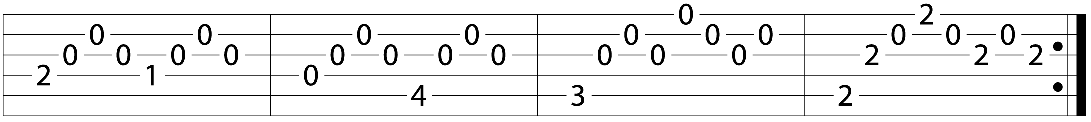
\includegraphics[width=365pt ]{res/sloni3-1.pdf}
\end{figure}
\vskip 25pt 
\begin{figure}[h]
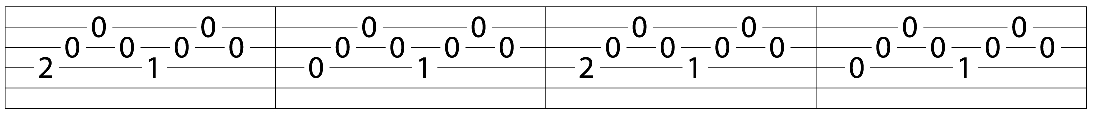
\includegraphics[width=365pt ]{res/sloni3-2.pdf}
\end{figure}
\vskip -8pt
\noprint{\Em{}}Vím o ces\noprint{\Eb[+]{}}tách, po kte\noprint{\G[/D]{}}rých chodí \noprint{\Eb[+]{}}sloni \noprint{\Em{}}pít,\noprint{\hskip 1.3em \Eb[+]{} \hskip 2.2em \G[/D]{} \hskip 2.5em \Eb[+]{}}\\
\begin{figure}[h]
\vskip 2ex
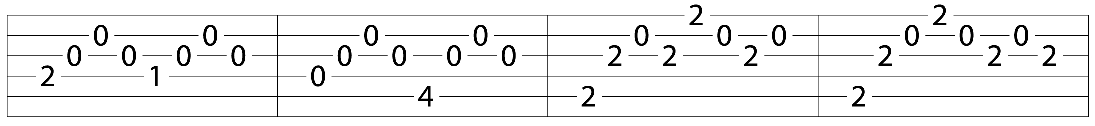
\includegraphics[width=365pt ]{res/sloni3-3.pdf}
\vskip -2ex
\end{figure}
\noprint{\Em{}}jsou žízní \noprint{\Eb[+]{}}rozryté, \noprint{\G[/D]{}}váhám, zda \noprint{\Db[dim]{}}dál mám \noprint{\H[7]{}}jít.\noprint{\hskip 2em \H[7]{}}\\
\begin{figure}[h!]
\vskip 2ex
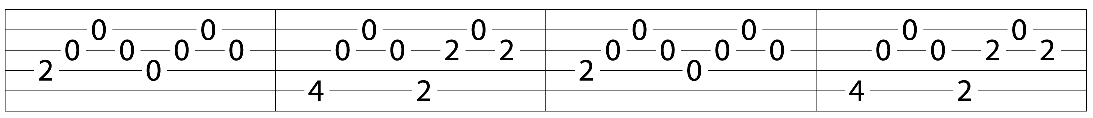
\includegraphics[width=365pt ]{res/sloni3-4.pdf}
\vskip -2ex
\end{figure}
\textls[-10]{\noprint{\Em{}}Na konci \noprint{\G[/D]{}}nečeká tů\noprint{\Db[dim]{}}ň s vodou \noprint{\H[7]{}}spásnou, \noprint{\\}\noprint{\Em{}}na konci \noprint{\G[/D]{}}poslední\noprint{\Db[dim]{}} naděje \noprint{\hskip 1em\H[7]{}}zhasnou,}\\
\begin{figure}[h!]
\vskip 2ex
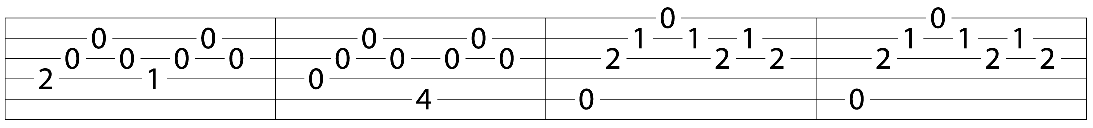
\includegraphics[width=365pt ]{res/sloni3-5.pdf}
\vskip -2ex
\end{figure}
už \noprint{\Em{}}vím, kde \noprint{\Eb[+]{}}leží \noprint{\hskip 1em \G[/D]{}}sloní \noprint{\hskip 1em\Db[dim]{}}hřbitov, \noprint{\\}\noprint{\Am{}}vím, kde najdeš kosti sluncem \noexport{\\}
\begin{figure}[h!]
\vskip 2ex
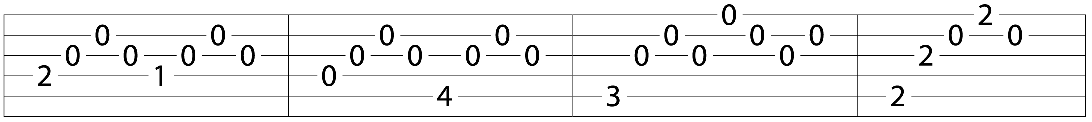
\includegraphics[width=365pt ]{res/sloni3-7.pdf}
\vskip -2ex
\end{figure}
\noprint{\Em{}}vyprah\noprint{\CHORD{\dots}{}}lé\ldots{}

\clearpage
\begin{figure}[h!]
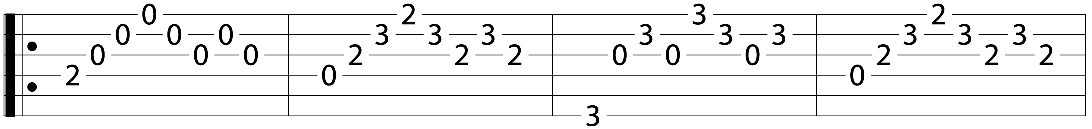
\includegraphics[width=365pt ]{res/sloni3-8.pdf}
\vskip -2ex
\end{figure}
Až nám \noprint{\Em{}}hvězdy přestanou \noprint{\D{}}svítit, až nám \noprint{\G{}}slunce přestane \noprint{\D{}}hřát,\\
\begin{figure}[h!]
\vskip 2ex
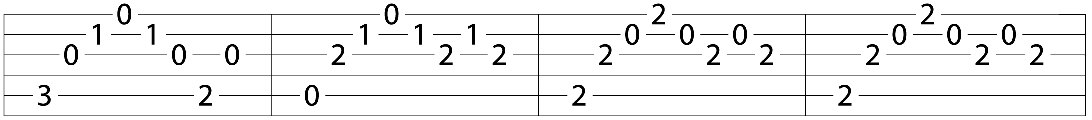
\includegraphics[width=365pt ]{res/sloni3-9.pdf}
\vskip -2ex
\end{figure}
až se \noprint{\C{}}budeme vesmírem \noprint{\Am{}}řítit, napo\noprint{\H[7]{}}řád\ldots{}\\
\begin{figure}[h!]
\vskip 2ex
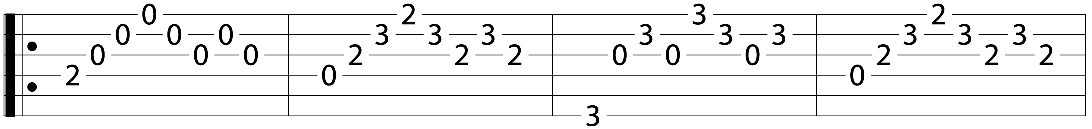
\includegraphics[width=365pt ]{res/sloni3-8.pdf}
\vskip -2ex
\end{figure}
Až mi \noprint{\Em{}}hvězdy přestanou \noprint{\D{}}svítit, až mi \noprint{\G{}}slunce přestane \noprint{\D{}}hřát,\\
\begin{figure}[h!]
\vskip 2ex
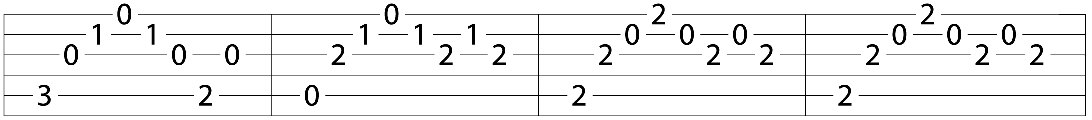
\includegraphics[width=365pt ]{res/sloni3-9.pdf}
\vskip -2ex
\end{figure}
chci se \noprint{\C{}}s vámi vesmírem \noprint{\Am{}}řítit, napo\noprint{\H[7]{}}řád,\noexport{\\}
\begin{figure}[h!]
\vskip 2ex
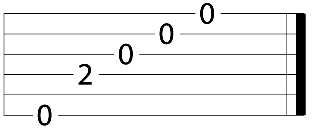
\includegraphics[scale=0.65 ]{res/sloni3-10.pdf}
\vskip -2ex
\end{figure}
napo\noprint{\Em{}}řád.
}
\Large
\crdheight=2.2ex
\toftagthis{filmove}
\song{Slunečný hrob}{Blue Effect}{35pt}{0.80}{
\rec{Usínám a chtěl bych se vrátit\\
o nějakej ten rok zpátky,
bejt zase malým klukem,\\
kterej si rád hraje a~který je s tebou.}

\vskip -1ex
\leftskip 70pt
\verse{1}\E{}Zdá se \Fsm{}mi, \hskip 1em \Gsm{} je to \hskip 0.4em \Fsm{}moc let,\\
já byl kluk, kterej chtěl\\
znáti svět, s tebou jsem si hrál.\\
\verse{*}\textbf{\sffamily G6 \hskip 0.5em F$\sharp$7 \hskip 0.5em Fmaj7}

\verse{2}Vrátím se a chtěl bych rád\\
být s tebou, zavzpomínat,\\
\E{}mám tu \Fsm{}teď \hskip 1em \Gsm{} ale \hskip 1em \Fsm{}zprávu \E{}zlou\E{}. \hskip 1em \E[7]{} \hskip 1.8em \E[7]{}

\chorus{}\Csm{}Su \hskip 0.3em - \hskip 0.3em \Dsm{}chá \hskip 1em \A{}hlína \Gsm{}ta - dy, \hskip 0.2em \Fsm{}\\
bez kvítí, bez vody,\\
\Gsm{} já na ni \Fsm{}poklekám,\\
\Gsm{}vzpomínkou po\H{}cta se vzdává.

\verse{3}Loučím se a něco však\\
tam zůstalo z těch našich dnů,\\
já teď vím, věrný zůstanu.\\
\textbf{R:}

\vskip -1ex
\verse{4}Loučím se\dots

\leftskip 35pt
\rec{Nemohu spát, probouzím se a zase se nemohu ubránit\\ myšlence,vrátit se o nějakej ten rok zpátky, bejt zase\\
malým klukem, kterej si rád hraje, který je s \emph{\E[9]{}}tebou.}
}



\toftagthis{olympic}
\song{Slzy tvý mámy}{Olympic}{20pt}{1}{
\capo{3}
\verse{1}\Em{}Chvilku vzpomínej,\Am{} je to všechno jen pár let,\\
\D{}na kytaru v duchu hrej,\G{} tvoje parta \G[/F$\sharp$]{}je tu hned.\\
\Em{}Z cigaret je modrej dým, \E[7]{}hraje magneťák,\\
\Am{}holka sedla na tvůj klín, \Em{}nevíš ani \Hm{}jak,\\
nevíš \Em{}jak.\hskip 1em \D{} \hskip 1em \Em{} \hskip 2em \D{}

\verse{2}Tvý roky bláznivý chtěly křídla pro svůj let,\\
dnes už možná nevíš sám, proč tě tenkrát pálil svět.\\
Chtěl jsi prachy na mejdan, byl to hloupej špás,\\
když jsi v noci vyšel ven, snad ses trochu třás, trochu třás.

\verse{*}\E{}Když tě našel noční \D{}hlídač,\\
byl by \C{}to jen příběh \G{}bláznivýho kluka,\\
\C{}nebejt nože \G{}ve tvejch dětskej rukách,\\
\C{}nebejt strachu \G{}mohlo to bejt \D{}všechno \Em{}jináč.\H[7]{}

\chorus{}\Em{}Slzy tvý mámy \D{}šedivý \Hm{}stékají na \Em{}polštář,\\
\C{}kdo tě zná, se vůbec \D{}nediví, že stárne \G{}její tvář.\H[7]{}\\
\Em{}Nečekej úsměv od ženy, který jsi \Am{}všechno vzal,\Am[/G]{}\\
jen pro tvý \Em{}touhy zborcený, \D{}léta ztrace\Hm{}ný,\\
ty oči \Em{}pláčou dál.

\verse{3}Když jsi vyšel ven, ze žalářních vrat,\\
možná, že jsi tenkrát chtěl znovu začínat.\\
Poctivejma rukama, jako správnej chlap,\\
snad se někdo ušklíb jen,\\
že jsi křivě šláp, křivě šláp.

\verse{*}I když byl někdo k tobě krutej,\\
proč jsi znovu začal mezi svejma,\\
tvůj pocit křivdy se pak těžko smejvá,\\
když hledáš vinu vždycky jenom v druhejch.\\
\textbf{R:}

}


\toftagthis{spiritual}
\song{Soudný den}{Spirituál kvintet}{55pt}{1}{
\verse{1}\Am{}Zdál se mi sen, že se nebe hroutí,\\
\G{}zdál se mi sen o poslední pouti,\\
\Am{}zdál se mi sen, že všechno seberou ti\\
v ten \Em{}soudný \Am{}den.

\verse{2}Kam běžet mám, Slunce rychle chladne,\\
kam běžet mám, měsíc na zem spadne,\\
kam běžet mám, moře už je na dně\\
v ten soudný den.

\verse{3}Stůj, nechoď dál, času už je málo,\\
stůj, nechoď dál, míň, než by se zdálo,\\
stůj, nechoď dál, otevři se, skálo,\\
v ten soudný den.

\verse{4}Pán tě zavolá, má pro každého místo,\\
Pán tě zavolá, jen kdo má duši čistou,\\
Pán tě zavolá, sám nedokázal bys to\\
v ten soudný den.

\verse{5}Soudí, soudí pány, slouhy,\\
soudí, soudí hříšné touhy,\\
\Am{}soudí, soudí, výčet pouhý, \Am{}á\ldots \hskip 0.5em  \A[sus2]{} \hskip 3em \E[sus4]{} \hskip 3em \E{}

\verse{*}\Am{}Vtom se probudíš, to byl jen sen,\\
\F{}vtom se probudíš, to byl jen sen,\\
\Dm[6]{}vtom se probudíš, to byl jen sen,\\
\Am{}jen \hskip 1em \E{}pouhý \Am{}sen.

\verse{6} Zdál se mi sen, že se nebe hroutí \dots

\verse{7}Zdál se mi sen, já stojím na svém místě,\\
zdál se mi sen, mé svědomí je čisté,\\
\Am{}zdál se mi sen, jen jedno vím \F{}jistě:\\
\Am{} je \hskip 1em  \E{}soudný \Am{}den!
~\\}


\toftagthis{anglicke}
\song{Sound of Silence}{Simon \& Garfunkel}{45pt}{1}{
\capo{6}
\verse{1}\Am{}Hello darkness, my old \G{}friend,\\
I've come to talk with you \Am{}again,\\
because a vision softl\F{}y cree\C{}ping\\
left its seeds while I w\F{}as slee\C{}ping\\
and the \F{}vision that was planted in my \C{}brain\\
still re\C{}mains\Am{}\\
\C{}within the \G{}sound of \Am{}silence.

\verse{2}In restless dreams I walked alone,\\
narrow streets of cobblestone.\\
'Neath the halo of a street lamp,\\
I turned my collar to the cold and damp,\\
when my eyes were stabbed by\\
the flash of a neon light,\\
that split the night\\
and touched the sound of silence.

\verse{3}And in the naked light I saw\\
ten thousand people, maybe more.\\
People talking without speaking,\\
people hearing without listening,\\
people writing songs that voices never share\\
and no one dared\\
disturb the sound of silence.

\verse{4}\uv{Fools,} said I, \uv{You do not know,\\
silence like a cancer grows.\\
Hear my words that I might teach you,\\
take my arms that I might reach you.}\\
But my words like silent raindrops fell\\
and echoed in the wells of silence

\verse{5}And the people bowed and prayed\\
to the neon god they made.\\
And the sign flashed out its warning\\
in the words that it was forming.\\
And the sign said: `The words of the prophets\\
are written on the subway walls\\
and tenement halls\\
and whispered in the sound of silence.'\\
}


%\toftagthis{anglicke}
%\song{Stairway to Heaven}{Led Zeppelin}{10pt}{1}{
%\vskip 8pt
%\verse{1}There's a lady who's sure, all that glitters is gold\\
%and she's buying a stairway to heaven.\\
%\textls[-17]{When she gets there she knows, if the stores are all closed}\\
% with a word she can get what she came for.\\
% Ooh, ooh, and she's buying a stairway to heaven.
%
%\verse{2}There's a sign on the wall but she wants to be sure,\\
% 'cause you know sometimes words have two meanings.\\
% In a tree by the brook, there's a songbird who sings,\\
% sometimes all of our thoughts are misgiven.
%
% Ooh, it makes me wonder,\\
%ooh, it makes me wonder.
%
%\verse{3}There's a feeling I get when I look to the west\\
%and my spirit is crying for leaving.\\
%\textls[-25]{In my thoughts I have seen rings of smoke through the trees}\\
%and the voices of those who stand looking.
%
% Ooh, it makes me wonder,\\
% ooh, it really makes me wonder.
%
%\verse{4}And it's whispered that soon, if we all call the tune,\\
% then the piper will lead us to reason.\\
% And a new day will dawn for those who stand long,\\
%and the forests will echo with laughter.
%\clearpage
%\verse{5}\textls[-15]{If there's a bustle in your hedgerow, don't be alarmed now,}\\
% it's just a spring clean for the May queen.\\
%\textls[-15]{Yes, there are two paths you can go by, but in the long run}\\
% there's still time to change the road you're on.\\
% And it makes me wonder.
%
%\verse{6}\textls[-45]{Your head is humming and it won't go, in case you don't know,}\\
% the piper's calling you to join him.\\
%\textls[-15]{Dear lady, can you hear the wind blow and did you know}\\
%your stairway lies on the whispering wind?
%
%\verse{7} And as we wind on down the road,\\
% our shadows taller than our soul.\\
%There walks a lady we all know,\\
%who shines white light and wants to show,\\
%how everything still turns to gold\\
%and if you listen very hard,\\
%the tune will come to you at last,\\
%when we all are one and one is all,\\
%to be a rock and not to roll.
%
% And she's buying the stairway to heaven.\\
%}


\toftagthis{anglicke}
\song{Stand By Me}{Ben E. King}{30pt}{1}{
\verse{1}When the \A{}night has come\Fsm{} and the land is dark\\
and the \D{}moon is the \E{}only light we'll \A{}see,\\
no I won't be afraid, oh, I won't be afraid,\\
just as long as you stand, stand by me.

\chorus{}So darling, darling,\\
stand by me, oh stand by me,\\
oh stand, stand by me, stand by me.

\verse{2}If the sky that we look upon should tumble and fall,\\
all the mountains should crumble to the sea,\\
I won't cry, I won't cry, no, I won't shed a tear,\\
just as long as you stand, stand by me.

\chorus{}And darling, darling,\\
stand by me, oh stand by me,\\
oh stand now, stand by me, stand by me.

\chorus{}So darling, darling,\\
stand by me, oh stand by me,\\
oh stand now, stand by me, stand by me.\\
Whenever you're in trouble won't you stand by me,\\
oh stand by me, oh won't you stand now, stand,\\
stand by me\\
}


\toftagthis{spiritual}
\song{Stará archa}{Spirituál kvintet}{60pt}{0.9}{
\chorus{}\revrpt{} Já mám \D{}kocábku náram-, \A[7]{}náram-, \D{}náram-,\\
kocábku náram-, \A[7]{}náram\D{}nou. \rpt{}

\verse{1}\D{}Pršelo a blejskalo se sedm neděl,\\
kocábku náram-, \A[7]{}náram\D{}nou,\\
Noe nebyl překvapenej, on to věděl,\\
kocábku náram-, \A[7]{}náram\D{}nou.\\
\textbf{R:}

\verse{*}\D{}Archa má cíl, archa má směr,\\
plaví se k Araratu \A[7]{}na se\D{}ver.\\
\textbf{R:}

\verse{2}Šem, Nam a Jafet byli bratři rodní,\\
kocábku náram-, náramnou,\\
Noe je zavolal ještě před povodní,\\
kocábku náram-, náramnou.

\verse{3}Kázal jim naložiti ptáky, savce,\\
kocábku náram-, náramnou.\\
\uv{Ryby nechte, zachrání se samy hladce,}\\
kocábku náram-, náramnou.\\
\textbf{R:, *., R:}

\verse{4}Přišla bouře, zlámala jim pádla, vesla,\\
kocábku náram-, náramnou,\\
tu přilétla holubice, snítku nesla,\\
kocábku náram-, náramnou.

\verse{5}Na břehu pak vyložili náklad celý,\\
kocábku náram-, náramnou,\\
ještě že tu starou dobrou archu měli,\\
kocábku náram-, náramnou.\\
\textbf{R:, *., R:, R:}\\
}

\toftagthis{spiritual}
\song{Starý příběh}{Spirituál kvintet}{50pt}{0.89}{
\verse{1}Řek' \D{}Mojžíš jednou lidu svému: Přišel čas,\\
dnes v noci tiše \Fsm{}vytratí se \G{}každý \A[7]{}z vás,\\
\D{}mává\D[7]{}, \hskip 1em \G{}mává\Gs[dim]{} \hskip 1em nám \D{}všem \A[7]{}svobodná \D{}zem.

\verse{2}Já říkám rovnou, každý ať s tím počítá,\\
že naše cesta ke štěstí je trnitá,\\
mává, mává nám všem svobodná zem.\\
\chorus{}\revrpt{} A \D{}kdo se bojí vodou jít,\\
ten podle tónů faraónů musí \A[7]{}žít,\\
\D{}mává\D[7]{}, \hskip 1em  \G{}mává\Gs[dim]{} \hskip 1em  nám \D{}všem \A[7]{}svobodná \D{}zem. \rpt{}

\verse{3}Až první krůček bude jednou za námi,\\
už nikdo nesmí zaváhat, dát na fámy,\\
mává, mává nám všem svobodná zem.

\verse{4}Pak tenhle vandr všem potomkům ukáže,\\
že šanci má jen ten, kdo má dost kuráže,\\
mává, mává nám všem svobodná zem.\\
\textbf{R:}

\verse{5}Ten starý příběh z bible vám tu vykládám,\\
ať každý ví, že rozhodnout se musí sám,\\
mává, mává nám všem svobodná zem.\\
\textbf{R:}\\
}

\toftagthis{nedvedi}
\song{Stánky}{Nedvědi}{55pt}{1}{
\verse{1}\D{}U stánků \G{}na levnou krásu,\\
\D{}postávaj' a \Gm{}smějou se času\\
\D{}s cigaretou a \A[7]{}s holkou, co nemá kam j\D{}ít.

\verse{2}Skleniček pár a pár tahů z trávy,\\
uteče den, jak večerní zprávy,\\
neuměj' žít a bouřej' se a neposlouchaj'.

\chorus{}\D[7]{} Jen\G{} zahlídli svět, maj' \A[7]{}na duši vrásky,\\
tak \D{}málo je, tak \Gm{}málo je lásky,\\
\D{}ztracená víra \A[7]{}hrozny z vinic neposbír\D{}á.

\verse{3}U stánků na levnou krásu,\\
postávaj' a ze slov a hlasů\\
poznávám, jak málo jsme jim stačili dát.\\
\textbf{R: $(2\times)$}\\
}


\song{Stín katedrál}{Karel Svoboda}{40pt}{1}{
\verse{1}\A{}Stín \D{}katedrál, \A{}půl nebe s bůhví \G{}čím, \D{}jé \E{}jé,\\
\A{}svůj \D{}ideál, \A{}sen, co si \H[7]{}dávám \E{}zdát.\E[7]{}\\
Z úsměvů šál, dům nebo básní rým, jéjé\\
jé, co ti dál, mám, řekni, dárkem dát.

\chorus{}\C{}Přej si, co \D{}chceš, zlatý \G{}důl nebo \D{}věž,\\
sladkou \C{}sůl, smutný \D{}ráj, suchý \G{}déšť. \G{}\\
\C{}Ber, tady \D{}máš mořskou \G{}pláň nebo \D{}pláž,\\
hudbu \C{}sfér, jenom \D{}ber se mnou \E{}též, \Hm[7]{}jé \hskip 1.8em \E[7]{}jé.

\verse{2}\A{}Můj \D{}ideál, \A{}víš, to co já mám \G{}rád, \D{}jé \E{}jé,\\
\A{}stín \D{}katedrál, \A{}sen, co si \H[7]{}k ránu \D{}dá - \E[7]{}vám \A{}zdát.\\
\textbf{R:}

\verse{3} Můj ideál, víš \dots

\revrpt{} \H[7]{}Sen, co se \E{}nám bude \A{}zdát. \rpt{}\\
}


\toftagthis{anglicke}
\song{Suicide is Painless}{M*A*S*H theme}{60pt}{1.05}{
\vskip 8pt
\verse{1}Through \Dm[7]{}early morning \G[7]{}fog I see\\
\C[maj]{}visions of the \Am[7]{}things to be,\\
the \Dm[7]{}pains that are with\G[7]{}held for me,\\
I \C{}realize and \Am[7]{}I can see\A[7]{}.

\chorus{}That \Dm[7]{}suicide is \G[7]{}painless,\\
it \C[maj]{}brings on many \Am[7]{}changes\\
and \F[maj]{}I can \Am{}take or \Dm[7]{}leave it \G[7]{}if I \Am{}please.

\verse{2}Try to find a way to make\\
all our little joys relate\\
without that ever present hate,\\
but now I know that it's too late.\\
And\ldots{}+ \textbf{R:}

\verse{3}The game of life is hard to play,\\
I'm going to lose it anyway,\\
the losing card I'll someday lay,\\
so this is all I have to say.\\
That\ldots{}+ \textbf{R:}
\clearpage
\verse{4}The only way to win is cheat\\
and lay it down before I'm beat\\
and to another give a seat\\
for that's the only painless feat.\\
'Cause\ldots{}+ \textbf{R:}

\verse{5}The sword of time will pierce our skins,\\
it doesn't hurt when it begins,\\
but as it works it's way on in,\\
the pain grow stronger watch it grin.\\
For\ldots{}+ \textbf{R:}

\verse{6}A brave man once requested me\\
to answer questions that are key,\\
is it to be or not to be\\
and I replied \uv{Oh, why ask me.}\\
'Cause\ldots{}+ \textbf{R:}

And you can do the same thing if you please.\\
}


\toftagthis{ceskekapely}
\song{Svařák}{Harlej}{50pt}{1}{
\verse{1}\G{}Když jsem sám doma, \Am{}poslouchám Vávra,\\
\C{}starýho vola, \D{}pořád dokola.\\
\G{}Chce to mít nápad, \Am{}a né pořád chrápat,\\
\C{}já dostal jsem nápad, \D{}udělat mejdan.

\chorus{}Mám \G{}rád svařené \Am{}víno červené,\\
já mám \C{}rád, rád sva\G{}řák.\\
Mám \G{}rád svařené \Am{}víno červené,\\
já mám \C{}rád, rád sva\G{}řák.

\verse{2}Se známou partou, domluva krátká,\\
zejtra v 6 hodin, vstup jedna lampa.\\
Začíná mejdan, na 200 \%,\\
my plníme plány, rostou nám blány.\\
\textbf{R: $(2\times)$}\\
}



\toftagthis{ceskekapely}
\song{Svaz českých bohémů}{Wohnout}{20pt}{1}{
\capo{1}
\medskip
\chorus\E{}Vracím se domů nad rá\Hm{}nem, kvalitním vínem omá\Fsm{}men,\\
z přímek se stávaj zatá\D{}čky, točí se \A{}svět, jsem na sra\E{}čky.\\
Vedle mě zvrací princezna, nastavím dlaň a požehnám,\\
pro všechny jasný poselství - tomu se říká přátelství. 

\verse{1}Mám tisíc otázek na žádnou vzpomínku,\\
skládám si obrázek kámen po kamínku.\\
Včerejší produkce šla do bezvědomí,\\
nastává dedukce, co na to svědomí. 

\verse{2}A už si vzpomínám, já byl jsem na srazu,\\
s kumpány který mám, patříme do svazu,\\
vlastníme doménu, tak si nás rozklikni,\\
svaz českejch bohémů\dots{}\\
\textbf{R:}

\verse{3}Stačí pár večírků, společně s bohémy,\\
za kterými se táhnou od školy problémy.\\
V partě je Blekota, Jekota, Mekota,\\
dost často hovoříme o smyslu života.

\verse{4}Jako je třeba teď, mám tisíc otázek,\\
na žádnou vzpomínku, si skládám obrázek.\\
Z těžkejch ran lížu se, včera jsme slavili,\\
svatýho Vyšuse.\\
\textbf{R:}\\

\verse{5}Svět zrychluje svý otáčky, sousedka peče koláčky.\\
Hlášen stav nouze nejvyšší, Hapkové volaj Horáčky.\\
Zástupy českejch bohému, vyráží ven do terénů\\
šavlí z kvalitního vína bojovat proti systému.

\revrpt{} Tak jsme se tu všichni sešli, co myslíš, osobo?\\
Na to nelze říci než \uv{Co je ti do toho?}\\
Tak jsme se tu všichni sešli, co myslíš, osude?\\
Na to nelze říci než \uv{Jinak to nebude.} \rpt\\
}


\toftagthis{anglicke}
\song{Sweet Home Alabama}{Lynyrd Skynyrd}{25pt}{0.93}{
\verse{1}\D{}Big \C{}wheels keep on \G{}turning,\G{}\\
carry me home to see my kin.\\
Singing songs about the Southland,\\
I miss Alabamy once again and I think it's a sin.

\verse{2}Well I heard mister Young sing about her,\\
well, I heard old Neil put her down.\\
Well, I hope Neil Young will remember,\\
a Southern man don't need him around anyhow.

\chorus{}Sweet home Alabama,\\
where the skies are so blue.\\
Sweet Home Alabama,\\
\D{}Lord, I'm \C{}coming home to \G{}you. \F{} \hskip 1em \C{}

\verse{3}In Birmingham they love the governor, \F{}boo \C{}hoo \D{}hoo!\\
Now we all did what we could do,\\
now Watergate does not bother me,\\
does your conscience bother you? Tell the truth.\\
\textbf{R:}

\verse{4}Now Muscle Shoals has got the Swampers\\
and they've been known to pick a song or two,\\
Lord, they get me off so much,\\
they pick me up when I'm feeling blue,\\
now how about you?\\
\textbf{R: $(2\times)$}
}


\toftagthis{hapka}
\song{Šaškové počmáraní}{Petr Hapka / Michal Horáček}{70pt}{1}{
\verse{1}\C{}Koukněte na toho \H[7]{}fintila,\\
\Dm{}pod krkem žlutého \G[7]{}motýla,\\
\Dm{}zelený klobouček \G[7]{}do týla\\
\D[7]{}šoupne si \G[7]{}na bílou \C{}pleš. \G[+]{}

\verse{2}I když ten tralalák padá mi,\\
hlavně že vyhrávám barvami,\\
hlavně že vyhrávám barvami,\\
\D[7]{}zase jsem \G[7]{}šťastnej jak \C{}veš.\C[7]{}

\chorus{}Co po mně \F{}chceš, pravdu či \Fm{}lež?\\
Zkus ty dvě \C{}rozeznat a pak se \C[7]{}směj,\\
barevný \F{}svět láme mi \Fm{}hřbet,\\
\Em{}přesto chci být \Eb[dim]{}šašek \hskip 0.7em \Dm[7]{}počmára\G[7]{}nej.

\verse{3}Ucho mi hryžou jak oplatku,\\
s rozběhem kopou mě do zadku,\\
tvrděj, že všechno je v pořádku,\\
když mi daj' mizernej plat.

\clearpage
\verse{4}Když ale koukám se na lidi,\\
všechno tak černě zas nevidím,\\
všechno tak černě zas nevidím,\\
ještě se dovedem smát.

\chorus{}Ne že se snad není co bát,\\
úzkost má tlapy jak Cassius Clay,\\
ten věčný strach na miskách vah,\\
převážit chce šašek počmáranej.

\verse{5}Kampak chcem ve věku rozumu\\
strkat prý své nosy na gumu,\\
určitě od rumu z konzumu\\
tak strašně červené jsou.

\verse{6}Ptám se však tebe, náš osude,\\
co bude, až tady nebude,\\
co bude, až tady nebude,\\
dojemně pitomá show.

\chorus{}Bláhová show, šaškové jdou\\
barevnou naději vytřískat z ní,\\
hledáme brod uprostřed vod,\\
my věční šaškové počmáraní.

\verse{7}Ptám se však tebe, náš osude,\\
co bude, až tady nebude,\\
co bude, až tady nebude,\\
dojemně pitomá show.\\
}


\toftagthis{nohavica}
\song{Šnečí blues}{Jaromír Nohavica}{60pt}{0.95}{
\verse{1}\G{}Jednou \C[7]{}jeden \G{}šnek \D[7]{}\\
\G{}šíle\C{}ně se \G{}lek',\D[7]{}\\
\G{}nikdo už dnes \G[7]{}neví, z \C{}čeho se tak \Cm{}zjevil,\\
že se\G{} dal hned \D{}na ú\G{}těk.\D[7]{}

\verse{2}Přes les a mýtinu\\
rychlostí půl metru za hodinu,\\
z ulity pára, ohnivá čára,\\
měl cihlu na plynu.

\verse{3}Ale v jedné zatáčce,\\
tam v mechu u svlačce,\\
udělal šnek chybu, nevyhnul se hřibu,\\
nevyhnul se bouračce.

\verse{4}Hned seběhl se celý les\\
a dali šneka pod pařez,\\
tam v tom lesním stínu, jestli nezahynul,\\
tak leží ještě dnes.

\verse{5}A kdyby použil vůz\\
anebo autobus,\\
\revrpt{} nebylo by nutné zpívat tohle smutné,\\
smutné šnečí blues. \rpt{}\\
}


\toftagthis{anglicke}
\song{Tears in Heaven}{Eric Clapton}{70pt}{0.85}{
\verse{1}\A{}Would you \E[/G$\sharp$]{} know my \Fsm{}name\\
\D[/F$\sharp$] if \hskip 0.2em I \hskip 0.2em s\A[/E]aw you in \E{}heaven?\\
Would it be the same\\
if I saw you in heaven?

\chorus{}\Fsm{}I must be \Cs[/F]{}strong,\A[7/E]{} and carry \Fs{}on,\\
'cause I \Hm[7]{}know I don't be\E[7sus4]{}long\\
here in hea\A{}ven.

\verse{2}Would you hold my hand\\
if I saw you in heaven?\\
Would you help me stand\\
if I saw you in heaven?

\chorus{}I'll find my way, through night and day,\\
'cause I know I just can't stay\\
here in heaven.

\verse{*}\C{}Time can \G[/H]{}bring you \Am{}down,\\
time can \D[/F$\sharp$]{}bend your \G{}knee.\D[/F$\sharp$]{} \hskip 2.5em \Em{} \hskip 2em \D[/F$\sharp$]{} \hskip 2.5em \G{}\\
Time can break your heart,\\
have you begging, please,\\
begging, please.\\
\vskip 7pt
(instrumental)\\
\vskip 10pt

\clearpage
\chorus{}Beyond the door,\\
there's peace I'm sure.\\
And I know there'll be no more\\
tears in heaven.

\verse{3. = 1}\\
\textbf{R: + }Cause I know I don't belong\\
here in heaven.\\}




\toftagthis{folk}
\songWithTranslation{czech}{
\song{Ten vítr to ví}{Waldemar Matuška}{70pt}{0.85}{
\crdheight=2.0ex
\verse{1}\D{}Míle a \G{}míle jsou \D{}cest, které znám,\\
jdou trávou i \G{}úbočím \A{}skal,\\
\D{}jsou cesty \G{}zpátky a \D{}jsou cesty \Hm{}tam\\
a \D{}já na všech \G{}s vámi \A{}stál.\A[7]{}\\
\D{}Proč ale \G{}blátem nás \D{}kázaly vést\\
a špínou nám \G{}třísnily \D{}šat?

\vskip -1.5ex
\chorus{}To \G{}ví snad jen \A{}déšť a \D{}vítr kolem \Hm{}nás,\\
ten \G{}vítr, co \A[7]{} začal právě \D{}vát.

\verse{2}Míle a míle se táhnou těch cest\\
a dál po nich zástupy jdou.\\
Kříže jsou bílé a lampičky hvězd\\
jen váhavě svítí tmou.\\
Bůh ví, co růží, jež dál mohly kvést,\\
spí v hlíně těch práchnivých blat?\\
\textbf{R:}

\verse{3}Dejte mi stéblo a já budu rád,\\
i stéblo je záchranný pás.\\
Dejte mi flétnu a já budu hrát\\
a zpívat a ptát se vás:\\
Proč jen se účel tak rád mění v bič\\
a proč že se má člověk bát ?\\
\textbf{R:}\\
}
}{english}{
\originalVersion{Blowin' in the Wind}{Bob Dylan}{60pt}{1}{
\verse{1}\noprint{\D{}}How many \noprint{\G{}}roads must a \noprint{\D{}}man walk down\\
before they \noprint{\G{}}call him a \noprint{\A{}}man?\\
\noprint{\D{}}How many \noprint{\G{}}seas must a \noprint{\D{}}white dove \noprint{\Hm{}}sail\\
be\noprint{\D{}}fore she \noprint{\G{}}sleeps in the \noprint{\A{}}sand?\noprint{\A[7]{}}\\
\noprint{\D{}}How many \noprint{\G{}}times must the \noprint{\D{}}cannon balls fly\\
before they're \noprint{\G{}}forever \noprint{\D{}}banned?

\chorus{}The \noprint{\G{}}answer, my \noprint{\A{}}friend, is \noprint{\D{}}blowin' in the \noprint{\Hm{}}wind,\\
the \noprint{\G{}}answer is \noprint{\A[7]{}}blowin' in the \noprint{\D{}}wind.

\verse{2}How many years can a mountain exist\\
before it is washed to the sea?\\
How many years can some people exist\\
before they're allowed to be free?\\
How many times can a man turn his head\\
and pretend that he just doesn't see?\\
\textbf{R:}

\verse{3}How many times must a man look up\\
before he can see the sky?\\
How many ears must one man have\\
before he can hear people cry?\\
How many deaths will it take 'til he knows,\\
that too many people have died?

\chorus{}The answer, my friend, is blowin' in the wind.\\
The answer is blowin' in the wind.\\
The answer is blowin' in the wind.\\ 
}
}



\toftagthis{folk}
\song{To tá Heľpa}{lidová}{30pt}{1}{
\verse{1}\Am{}To ta \Dm{}Heľpa, \Am{}to ta \Dm{}Heľpa, \Am{}to je \E{}pekné \Am{}mesto.\\
A v tej Heľpe, a v tej Heľpe švárnych chlapcov je sto.\\
\revrpt{} \F{}Koho je sto, \C{}toho je sto, \G{}nie po mojej \C{}vôli\E{},\\
\Am{}ľen za \Dm{}jedným, \Am{}ľen za \Dm{}jedným, \Am{}srdiečko \E{}ma \Am{}bolí. \rpt{}

\verse{2}Za Janíčkom, za Palíčkom, krok by nespravila,\\
za Ďuríčkom, za Mišíčkom, Dunaj preskočila.\\
\revrpt{} Dunaj, Dunaj, Dunaj, Dunaj, aj to širé more,\\
ľen za jedným, ľen za jedným, počešenie moje. \rpt{}\\
}


\toftagthis{anglicke}
\song{Total Eclipse of the Heart}{Bonnie Tyler}{12pt}{1}{
\verse{1}\Am{}Turn around, every now and then I get a \G{}little bit\\
lonely and you're never coming round.\\
Turn around, every now and then I get a little bit\\
tired of listening to the sound of my tears.

\vskip -2ex
\C{}Turn around, every now and then I get a \Bb{}little bit\\
nervous that the best of all the years have gone by.\\
Turn around, every now and then I get a little bit\\ 
terrified and then I see the look in your eyes.

\vskip -2ex
\scalebox{.97}[1.0]{\Eb{}Turn around, \Ab[maj7]{}bright eyes, every now and then I fall apart.}\\
\scalebox{.97}[1.0]{\Eb{}Turn around, \Ab[maj7]{}bright eyes, every now and then I fall a\Am{}part.}

\verse{2}Turn around, every now and then I get a little bit\\
restless and I dream of something wild.\\
Turn around, every now and then I get a little bit\\ 
helpless and I'm lying like a child in your arms.

Turn around, every now and then I get a little bit\\ 
angry and I know I've got to get out and cry.\\
Turn around, every now and then I get a little bit\\ 
terrified but then I see the look in your eyes.

Turn around bright eyes, every now and then I fall apart.\\
Turn around bright eyes, every now and then I fall a\G{}part.

\scalebox{.95}[1.0]{\chorus{}And I \Em{}need you now \C{}tonight, and I \D{}need you more than \G{}ever}\\
\scalebox{.95}[1.0]{And if you'll only hold me tight, we'll be holding on forever.}\\
\scalebox{.95}[1.0]{And we'll only be making it right, cause we'll \D{}never be wrong} 

To\Em{}gether we can take it to the \D{}end of the line,\\
your \Em{}love is like a shadow on me \A{}all of the time.\\
I \G{}don't know what to do and I'm \D{}always in the dark,\\
we're \Em{}living in a powder keg and \A{}giving off sparks.

I really need you to\G{}night, for\D{}ever's gonna \Hm{}start to\C{}night,\\
for\D{}ever's gonna start tonight.

\verse{*}\G{}Once upon a time I was \Em[7]{}falling in love,\\
but \Hm{}now I'm only falling a\C{}part,\\
there's \Am{}nothing I can do, a \D{}total eclipse of the \G{}heart.

Once upon a time there was light in my life,\\
but now there's only love in the dark,\\
nothing I can say, a total eclipse of the heart 
}


\toftagthis{filmove}
\song{Trezor}{Karel Gott}{5pt}{1}{
\D{}Ze zdi na mě \D[7]{}tupě zírá \G{}po trezoru temná díra,\\
\E[7]{}poznám tedy bez nesnází, \A[7]{}že tam nepochybně něco schází,\\
\D{}ve zdi byl totiž \D[7]{}po dědovi \G{}velký trezor ocelový.\\
\A[7]{}Mám tedy ztrátu zdánlivě minimál\G[7]{}ní. \hskip 0.8em \D{}

Na to, že \A[7]{}náhodně v krámě vášnivé dámě\\
\D{}padl jsem za tro\Hm{}fej,\\
\E[7]{}tvrdila pevně: přijdu tě levně, \A[7]{}nezoufej, ó jé, jé, jé, jé.

\D{}Jenže potom \D[7]{}v naší vile \G{}chovala se zhůvěřile,\\
\textls[-45]{\E[7]{}aby měla správné klima, \A[7]{}dal jsem ji do trezoru, ať v klidu dřímá.}\\
\textls[-30]{\D{}Spánku se bráním \D[7]{}už noc pátou, \G{}ne ale žalem nad tou ztrátou,}\\
\A[7]{}jen hynu bázní, že kasař úlovek \G[7]{}vrá - \D{}tí.

Na to, že\ldots{}
}


%\toftagthis{matuska}
%\song{Třešně zrály}{Waldemar Matuška}{30pt}{0.85}{
%\verse{1}\C{}Jó, třešně zrály, \G[7]{}zrovna třešně \C{}zrály,\\
% \C{}sladký \E[7]{}třešně \Am{}zrály a \F{}teplej \G[7]{}vítr \C{}vál.\\
%A já k horám v dáli, k modrejm horám v dáli,\\
% sluncem, který pálí, tou dobou stádo hnal.\\
%\chorus{}\C{}Jó, \G[7]{}třešně \Am{}zrály, \Dm[7]{}zrovna \G[7]{}třešně \C{}zrály,\\
% \C{}sladký \E[7]{}třešně \Am{}zrá - \F{}ly a \Dm{}jak to \G[7]{}bylo \C{}dál? 
%
%\verse{2}Tam, jak je ta skála, ta velká bílá skála,\\
% tak tam vám holka stála a bourák opodál.\\
%A moc se na mě smála, zdálky už se smála,\\
% i zblízka se pak smála a já se taky smál.\\
%\textbf{R:}\\
%\verse{3}Řekla, že mě má ráda, už dlouho mě má ráda,\\
% dlouho mě má ráda, abych prej si ji vzal.\\
%Ať nechám ty svý stáda, že léta pilně střádá,\\
% jen abych ji měl rád a žil s ní jako král.\\
%\textbf{R:}\\
%\verse{4}Pokud je mi známo, já řek' jenom: \uv{Dámo,\\
% milá hezká dámo, zač bych potom stál.\\
% Ty můj typ nejsi, já mám svoji Gracie,\\
% moji malou Gracie, a tý jsem srdce dal.}\\
%\textbf{R:}\\
%\verse{5}Jó, u tý skály dál třešně zrály,\\
% modrý hory v dáli, teplej vítr vál.\\
%A já od tý skály, od tý bílý skály,\\
%v slunci, který pálí, jsem hnal svý stádo \C{}dá - \Ab{}á - \C{}ál.\\
%
%}

\toftagthis{folk}
\song{Tři kříže}{Hop Trop}{60pt}{0.95}{
\verse{1}\Dm{}Dávám sbohem \C{}břehům prokla\Am{}tejm,\\
který \Dm{}v drápech má \C{}ďábel \Dm{}sám.\\
\Dm{}Bílou přídí \C{}šalupa \uv{My \Am{}Grave}\\
míří \Dm{}k útesům, \C{}který \Dm{}znám.

\chorus{}Jen tři \F{}kříže z bí\C{}lýho kame\Am{}ní\\
někdo \Dm{}do písku \C{}posklá\Dm{}dal.\\
Slzy \F{}v očích měl a \C{}v ruce znave\Am{}ný\\
lodní \Dm{}deník, co \C{}sám do něj \Dm{}psal.

\verse{2}První kříž má pod sebou jen hřích,\\
samý pití a rvačky jen.\\
Chřestot nožů, při kterým přejde smích,\\
srdce kámen a jméno \uv{Stan}.\\
\textbf{R:}

\verse{3}Já, Bob Green, mám tváře zjizvený,\\
štěkot psa zněl, když jsem se smál.\\
Druhej kříž mám a spím pod zemí,\\
že jsem falešný karty hrál.\\
\textbf{R:}

\verse{4}Třetí kříž snad vyvolá jen vztek,\\
Fatty Rogers těm dvoum život vzal.\\
Svědomí měl, vedle nich si klek'\ldots{}

\rec{Snad se chtěl modlit: \uv{Vím, trestat je lidský,\\
ale odpouštět božský. Snad mi tedy Bůh odpustí.}}

\chorus{}Jen tři kříže z bílýho kamení\\
jsem jim do písku poskládal.\\
Slzy v očích měl a v ruce znavený\\
lodní deník, a v něm, co jsem psal.\\
}


\toftagthis{nohavica}
\song{U nás na severu}{Jaromír Nohavica}{70pt}{1}{
\verse{1}\Em{}V Bělském lese \Am{}toulají se \H[7]{}mamu\Em{}ti,\\
\G{}když je neo\D[7]{}solíš, tak jsou \G{}bez \C{}chu\H[7]{}ti,\\
\G{}nevěřil bys, \D[7]{}kolik to dá \G{}ro - \C{}bo - \H[7]{}ty\\
\Em{}zavařovat \Am{}na kyselo \H[7]{}chobo\Em{}ty.


\chorus{}Ďura \Am{}světa v každém směru,\\
co si \Em{}myslíš, na to seru,\\
nemluv, \H[7]{}bo mě mory beru,\\
tak se \Em{}žije tady na se\E[7]{}veru.

Větry fučí ze všech směrů,\\
když není máslo, jíme Heru,\\
furt dva metry od maléru,\\
tak se \Em{}žije \hskip 0.5em \H[7]{}tu u \Em{}nás.\\
Ná na nána \dots

\verse{2}Všude kolem ve světě jsou mobily,\\
u nás nevyroste ani obilí,\\
psi se živí výhonkama přesliček,\\
každá rodina má deset dětiček\\
\textbf{R:}

\verse{3}V centru vedle sochy T.G. Masaryka\\
ze země jak na Islandu voda stříká.\\
Malí, velcí, tlustí, tencí, různé rasy,\\
zadarmo si tady všichni myjou vlasy.\\
\textbf{R:}

\verse{4}Z Karolíny je vidět do Evropy,\\
pod Radhoštěm potkáš aj lidoopy,\\
po výplatě je tu velmi divoko,\\
Praha daleko a Pánbůh vysoko.\\
\textbf{R:}
}


\toftagthis{folk}
\song{Už to nenapravím}{Samson}{15pt}{1}{
\capo{2}
\chorus{}\Am{}Vap ta\D{}va d\F{}ap \E[7]{}\ldots \hskip 0.7em \Am{}

\verse{1}V \Am{}devět hodin dvacet pět \D{}mě opustilo štěstí,\\
ten \F{}vlak, co jsem jím měl jet, na koleji\E{} dávno \E[7]{}nestál.\\
V devět hodin dvacet pět jako bych dostal pěstí,\\
já za hodinu na náměstí měl jsem stát,\\
ale v jiným městě.

\verse{*}Tvá \A[7]{}zpráva zněla prostě a byla tak krátká,\\
že \Dm{}stavíš se jen na skok, že nechalas mi vrátka\\
\G{}zadní otevřená, \E{}zadní otevřená.

Já naposled tě viděl, když ti bylo dvacet,\\
to jsi tenkrát řekla, že se nechceš vracet,\\
že jsi unavená, ze mě unavená.\\
\textbf{R:}

\verse{2}Já čekala jsem, hlavu jako střep, a zdálo se, že dlouho,\\
může za to vinný sklep, že člověk často sleví.\\
Já čekala jsem, hlavu jako střep, s podvědomou touhou,\\
čekala jsem dobu dlouhou víc než dost,\\ 
kolik přesně, nevím.

\leftskip 30pt
\verse{*}Pak jedenáctá byla a už to bylo pasé,\\
já měla vědět dřív, že vidět chci tě zase,\\
láska nerezaví, láska nerezaví.

Ten list, co jsem ti psala, byl dozajista hloupý,\\
byl odměřený moc, na vlídný slovo skoupý,\\
už to nenapravím, už to nenapravím.\\
\textbf{R:}
}

\toftagthis{folk}
\songWithTranslation{czech}{
\song{Veď mě dál, cesto má}{Pavel Bobek}{30pt}{1}{
\verse{1}\D{} Někde v dálce\Hm{} cesty končí,\\
\A{} každá prý však \G{}cíl svůj \D{}skrývá.\\
Někde v dálce každá má svůj cíl,\\
ať je pár mil dlouhá nebo tisíc mil. 

\chorus{}Veď mě \D{}dál, cesto \A{}má, veď mě \Hm{}dál, vždyť i \G{}já\\
tam, kde \D{}končíš, chtěl bych \A{}dojít,\\
veď mě \G{}dál, cesto \D{}má. 

\verse{2}Chodím dlouho po všech cestách,\\
všechny znám je, jen ta má mi zbývá.\\
Je jak dívky, co jsem měl tak rád,\\
plná žáru bývá, hned zas samý chlad.\\
\textbf{R:}

\verse{*}\Hm{}Pak na pat\A{}ník posled\D{}ní napíšu \D{}křídou\\
\G{}jméno své a \D{}pod něj, že jsem \A{}žil \D{}hrozně \A{}rád.\\
\Hm{}Písně své, co mi \C{}v kapsách zbydou,\\
\G{}dám si bandou \D{}cvrčků hrát a \A{}půjdu spát, půjdu \A[7]{}spát.\\
\textbf{R: $(2\times)$}\\
}
}{english}{
\originalVersion{Take Me Home, Country Roads}{John Denver}{60pt}{1}{
\verse{1}\noprint{\D{}}Almost heaven,\noprint{\Hm{}} West Virginia\\
\noprint{\A{}}Blue Ridge Mountains, \noprint{\G{}}Shenandoah \noprint{\D{}}River\\
Life is old there, older than the trees\\
Younger than the mountains, growing like a breeze

\chorus{}Country \noprint{\D{}}roads, take me \noprint{\A{}}home\\
to the \noprint{\Hm{}}place I be\noprint{\G{}}long\\
West Vir\noprint{\D{}}ginia, Mountain \noprint{\A{}}Mama\\
Take me \noprint{\G{}}home, country \noprint{\D{}}roads

\verse{2}All my memories gather 'round her\\
Miner's lady, stranger to blue water\\
Dark and dusty, painted on the sky\\
Misty taste of moonshine, teardrop in my eye\\
\textbf{R:}

\verse{*}\noprint{\Hm{}}I hear her \noprint{\A{}}voice, in the \noprint{\D{}}mornin' hour she calls me\\
The \noprint{\G{}}radio re\noprint{\D{}}minds me of my \noprint{\A{}}home \noprint{\D{}}far a\noprint{\A{}}way\\
And \noprint{\Hm{}}drivin' down the \noprint{\C{}}road, I get a \noprint{\G{}}feelin\\
That I \noprint{\D{}}should have been home \noprint{\A{}}yesterday, yester\noprint{\A[7]{}}day\\
\textbf{R: $(2\times)$}\\
}
}



\toftagthis{ceskekapely}
\song{Velmi nesmělá}{Jablkoň}{30pt}{0.9}{
\verse{1}\Am{}Potkali se v pondělí,\G{} \hskip 1em \Am{} \hskip 1em byli velmi nesmělí\G{} \hskip 1em \E{}\\
\C{}a tak oba dělali,\G{} \hskip 1em \E{} \hskip 1em \Am{}jako by se neznali.\C{} \hskip 1em \E{} \hskip 1em \Am{}\\
\verse{2}V úterý sebral odvahu, odhodlal se k pozdravu\\
a pak v citové panice prchali oba k mamince. 

\chorus{}\C{}Sema\E{}for popásá\Am{} chodce\F{}, motorky, \C{}auta, \G{}tramva\C{}je\\
\C{}a všechny \E{}cesty dneska \Am{}vedou\F{} \hskip 0.8em \C{}do pekla i \G{}do rá\Am{}je,\\
\C{}do pekla i \G{}do rá\C{}je.

\verse{3}Ve středu spolu postáli, dívali se do dáli\\
a do dáli se dívali i když už spolu nestáli.\\
\verse{4}Ve čtvrtek přišel první zvrat, prohlásil že má ji rád\\
a ona špitla do ticha, že na ni moc pospíchá.\\
\textbf{R:} 

\verse{5}V pátek to vzal útokem, jak tak šli krok za krokem,\\
přesně v šestnáct dvacet pět zavadil loktem o loket.\\
\verse{6}V sobotu ji chyt za ruku, hlavou jí kmitlo je to tu\\
a jak hodiny běžely, drželi se drželi.\\
\textbf{R:}

\verse{7}V neděli už věděli, že jsou možná dospělí\\
a tak při sedmém pokusu dal jí pusu na pusu.\\
\verse{8}Když zas přišlo pondělí, tak příšerně se styděli,\\
\revrpt{} že oba dva dělali, jakoby se neznali. \rpt{}\\
}


\toftagthis{slovenske}
\song{Voda, čo ma drží nad vodou}{Elán}{25pt}{0.86}{
\crdheight=2.0ex
\verse{1}\E{}Keby bolo \A{}niečo, \H[/D$\sharp$]{}čo sa ti dá \E{}zniesť,\\
okrem neba \A{}nado mnou\Gsm{} a \hskip 1.7em \Fsm{} \hskip 2.2em \H{}miliónov \A[sus2]{}hviezd. \H{}\\
\E{}Tak by som to \A{}zniesol, \H{}vždy znova a \Gsm{}rád,\\
\A{}k tvojim nohám \E{}dobré veci\Fsm{} \hskip 0.3em ako \hskip 0.3em \H{}vodopád\A{}.

\verse{2}Keby som mal kráčať, sám a zranený,\\
šiel by som až tam, kde tvoja duša pramení.\\
Keby som ten prameň našiel náhodou,\\
bola by to voda, čo ma drží nad vodou.

\verse{*}\Gsm{} Môžeš zabud\Csm{}núť, \hskip 0.7em \A{} stačí kým tu \E{}si,\\
\Gsm{} iba ďalej \Csm{}buď, \hskip 0.5em \A{} nič viac nemu\H{}síš. \Gs[sus4]{}\\
\chorus{}Chcem sa z teba \Csm{}napiť, \hskip 0.5em \E{} šaty odhoď \H{}preč,\\
\Gs{} \hskip 1.2em \Gs[7]{}čo má byť sa \Csm{}stane, \H{}tak cez moje \A{}dlane\A[/G$\sharp$]{},\\
ako \Fsm{}čistý prameň teč.\Gs{}\\
Ak ťa ešte trápi smútok z rozchodov,\\
ono sa to podá, ty si predsa voda,\\
čo ma \Fsm{}drží nad vo\Fsm{}dou. \hskip 0.7em \H{}\\
\vskip 8pt
\verse{3}Keby bolo niečo\ldots\\
\textbf{R:}
}

\toftagthis{ceskekapely}
\song{Voda živá}{Aneta Langerová}{15pt}{1}{
\verse{1}Když \F{}končí se den a usne má zem, pak \C{}na malou chvíli\\
\F{}vrací se zpět můj niterný svět, co \C{}osud tvůj sdílí.\\
Do všech \Gm{}světových stran, do všech koutů co znám\Bb{} \hskip 1em \C{}\\
vo\F{}lám.

\verse{2}\textls[-10]{Když přichází noc, tak cítím, jak moc tvé světlo mi schází,}\\
\textls[-15]{promítne krátce svůj stín někde v dálce, tvá duše se ztrácí.}\\
Zdá se nezbylo nic, jenže čím dál tím víc\ldots{}

\chorus{}Ve mně navždy z\F{}ůstává tvoje voda živ\C{}á,\\
uvnitř odpočív\Dm{}á, čistá a důvěřiv\Bb{}á.\\
Ve mně navždy z\F{}ůstává tvoje voda živ\C{}á,\\
tiše odplouv\Dm{}á, čistá a důvěřiv\Bb{}á. \hskip 0.5em \C{}

\verse{3}Když končí se den a usne má zem, nevnímám čas,\\
vrací se zpět můj niterný svět, snad probudí nás.\\
Zdá se nezbylo nic, jenže čím dál tím víc\ldots{}\\
\textbf{R: $(2\times)$}
}


\toftagthis{anglicke}
\song{Wake Me Up When September Ends}{Green Day}{50pt}{1}{
\crdheight=2.5ex
\verse{1}\D{}Summer has \D[/C$\sharp$]{}come and passed,\\
\D[/H]{}the innocent can \D[/A]{}never last.\\
\G{}Wake me up \Gm{}when September \D{}ends.

\verse{2}Like my father's come to pass,\\
seven years has gone so fast.\\
\G{}Wake me up \Gm{}when September \D{}ends.\D[/C$\sharp$]{}

\chorus{}\Hm{}Here comes the \Fsm{}rain again,\\
\G{}falling from the \D{}stars,\D[/C$\sharp$]{}\\
\Hm{}drenched in my \Fsm{}pain again,\\
\G{}becoming who we \A{}are.

\verse{3}As my memory rests,\\
but never forgets what I lost.\\
Wake me up when September ends

\verse{4}Summer has come and passed\ldots 
\clearpage
\verse{5}Ring out the bells again\\
like we did when spring began.\\
Wake me up when September ends.\\
\textbf{R:}

\verse{6}As my memory rests\ldots 

\verse{7}Summer has come and passed\ldots 

\verse{8}Like my father's come to pass,\\
twenty years has gone so fast.\\
\revrpt{} Wake me up when September ends. \rpt{} $^{3\times}$

}


\toftagthis{anglicke}
\song{What a Wonderful World}{Louis Armstrong}{20pt}{1}{
\verse{1}I see \C{}trees of \Em{}green,\F{} red roses \Em{}too,\\
\Dm[7]{}I see them \C{}bloom,\E[7]{} for me and \Am{}you,\\
and I \Ab{}think to myself:\Dm[7]{} \uv{What a \G[7]{}wonderful wo\C{}rld.}\C[+]{} \hskip 1.5em \F[maj7]{} \hskip 3em \G[7]{}\\
\verse{2} I see skies of blue and clouds of white,\\
the bright blessed day, the dark sacred night\\
and I think to myself: \uv{What a wonderful wo\C{}rld}\F{} \hskip 0.8em \F{} \hskip 0.8em \C{}

\verse{*}The \G[7]{}colors of the rainbow, so \C{}pretty in the sky,\\
are \G[7]{}also on the faces of \C{}people goin' by.\\
I see \Am{}friends shaking \G[/H]{}hands, saying:\Am[/C]{} \uv{How do you \G{}do?}\\
\Am[/C]{}They're really \Cs[dim]{}saying: \uv{\Dm[7]{}I \hskip 2em \Cs[dim]{}love\hskip 1.7em \G[7]{}you.} 

\verse{3}I hear babies cry, I watch them grow,\\
they'll learn much more than I'll ever know,\\
and I think to myself: \uv{What a wonderful wo\C{}rld\Em[7b5]{}.}\\
\A[7]{}Yes, I \Dm[7]{}think to myself:\Dm[7/G]{} \uv{What a \G[7]{}wonderful \C{}world.}\F[6]{} \hskip 1.2em \C{}\\
}


\toftagthis{anglicke}
\song{While My Guitar Gently Weeps}{The Beatles}{35pt}{1.05}{
\medskip 

\verse{1}I \Am{}look at you \Am[/G]{}all, see the \D[9/F$\sharp$]{}love there that's \F{}sleeping,\\
\Am{}while my gui\G{}tar gently \D{}weeps.\E[7]{}\\
I \Am{}look at the \Am[/G]{}floor and I \D[9/F$\sharp$]{}see it needs \F{}sweeping,\\
\Am{}still my gui\G{}tar gently \C{}weeps.\E[7]{}

\chorus{}\A{}I don't know \Csm{}why \hskip 0.8em \Fsm{} nobody \Csm{}told you\\
\Hm{}how to unfold your \E{}love.\\
I don't know how someone controlled you,\\
they bought and sold you.

\verse{2}I look at the world and I notice it's turning,\\
while my guitar gently weeps.\\
With every mistake we must surely be learning,\\
still my guitar gently weeps.

\chorus{}I don't know how you were diverted,\\
you were perverted too.\\
I don't know how you were inverted,\\
no one alerted you.

\clearpage
\verse{3}I look from the wings at the play you are staging,\\
while my guitar gently weeps.\\
As I'm sitting here, doing nothing but ageing,\\
still, my guitar gently weeps.

\verse{4} I look at you all, see the love there that's sleeping,\\
while my guitar gently weeps.\\
Look at you all\ldots{}\\
still my guitar gently weeps.\\
}


\toftagthis{anglicke}
\song{Wonderwall}{Oasis}{20pt}{1}{
\vskip 10pt
\crdheight=2.5ex
\verse{1}\Em[7]{}Today is \G{}gonna be the day\\
that they're \D[sus4]{}gonna throw it back to \A[sus4]{}you.\\
By now, you should've somehow\\
realized what you gotta do.\\
I don't believe that anybody\\
feels the way I do about you \C[add9]now. \hskip 1.2em \D[sus4]{} \hskip 3em \A[7sus4]{}

\verse{2} Backbeat, the word is on the street\\ 
that the fire in your heart is out.\\
I'm sure you've heard it all before,\\
but you never really had a doubt.\\
I don't believe that anybody\\
feels the way I do about you now.

\verse{*}And \C[add9]{}all the roads we \D{}have to walk are \Em{}winding\\
and \C[add9]{}all the lights that \D{}lead us there are \Em{}blinding.\\
\C[add9]{}There are many \D{}things that I would \G{}like to \G[/F$\sharp$]{}say to \Em{}you,\\
but I don't know \A[7sus4]{}how.

\clearpage
\chorus{}Because \C[add9]{}maybe \hskip 0.7em \Em[7]{} \hskip 2.3em \G{}you're \Em[7]{}gonna be the one that\\
\C[add9]{}saves me\Em[7]{} \hskip 2.3em \G{}and \Em[7]{}after \hskip 0.5em \C[add9]{}all,\hskip 2em  \Em[7]{} \hskip 2.3em \G{}\\
you're my \Em[7]{}wonder\C[add9]{}wall. \hskip 1em \Em[7]{} \hskip 2.4em \G{} \hskip 1em \Em[7]{}

\verse{3}Today was gonna be the day,\\
but they'll never throw it back to you.\\
By now, you should've somehow\\
realized what you're not to do.\\
I don't believe that anybody\\
feels the way I do about you now.

\verse{*}And all the roads that lead you there were winding\\
and all the lights that light the way are blinding.\\
There are many things that I would like to say to you,\\
but I don't know how.

\textbf{R: $(2\times)$}~\\
I said maybe you're gonna be the one that saves me.\\
You're gonna be the one that saves me.\\
You're gonna be the one that saves me.\\
}


\toftagthis{anglicke}
\song{Yesterday}{The Beatles}{25pt}{1}{
\verse{1}\G{}Yesterday,\Fsm[7]{} all my \H[7]{}troubles seemed so \Em{}far away\Em[/D]{},\\
\C[maj]{}now it \D[7]{}looks as though they're \G{}here to stay, \G[/F$\sharp$]{}oh,\\
\Em[7]{} I be - \A[7]{}lieve in \C{}ye - \G{}sterday.

\verse{2}Suddenly, I'm not half the man I used to be,\\
there's a shadow hanging over me,\\
oh, I yesterday came suddenly.

\chorus{}\Fsm[7]{}Why \hskip 0.8em \H[7]{}she \Em{}had\ \ \D{}to \C{}go \H[7]{}I don't \D[7/A]{}know \D[7]{}she wouldn't \G{}say.\\
I said something wrong, now I long for yesterday.

\verse{3}Yesterday, love was such an easy game to play,\\
now I need a place to hide away,\\
oh, I believe in yesterday.\\
\textbf{R:}

\verse{4}Yesterday, love was such an easy game\dots

\G{}Mmm\ldots{}\A[7/G]{}mmm\ldots{}\C[/G]{}mmm\ldots{}\G{}mmm.\\
}


\toftagthis{folk}
\song{Zabili, zabili}{Miloš Štědroň}{65pt}{1}{
\verse{1}\C{}Zabili, \F{}zabili \Dm{}chlapa z Kolo\F{}čavy,\C{}\\
řekněte, hrobaři, kde je pochovaný. 

\chorus{}\C{}Bylo tu, není tu, havrani \F{}na plotu,\\
\C{}bylo víno v sudě, \F{}teď tam voda bude,\\
není, \C{}není tu. 

\verse{2}Špatně ho zabili, špatně pochovali,\\
vlci ho pojedli, ptáci rozklovali.\\
\textbf{R:}

\verse{3}Vítr ho roznesl po dalekém kraji,\\
havrani pro něho po poli krákají.\\
\textbf{R:}

\verse{4}Kráká starý havran, krákat nepřestane,\\
dokud v Koločavě živý chlap zůstane.\\
\ldots{}živý chlap zůstane.
}


\toftagthis{folk}
\song{Zafúkané}{Fleret}{20pt}{1}{
\verse{1}\Am{}Větr sněh \A[sus2]{}zanésl z \Am{}hor do po\A[sus2]{}lí,\\
\Am{}já idu \C{}přes kopce, \G{}přes údo\Am{}lí,\\
\C{}idu k tvej \G{}dědině \G{}zatúla\C{}nej,\\
\F{}cestičky \C{}sněhem sú \E{}zafúka\Am{}né.\hskip 1em \F[maj]{}\hskip 3em \Am{} \hskip 2em \E[sus4]{}

\chorus{}\Am{}Zafúka\C{}né, \G{}zafúka\C{}né, \F{}kolem mňa \C{}všecko je \Dm{}zafúka\E{}né,\\
\Am{}zafúka\C{}né, \G{}zafúka\C{}né, \F{}kolem mňa \C{}všecko je \E{}zafúka\Am{}né.

\verse{2}Už vašu chalupu z dálky vidím,\\
srdce sa ozvalo, bit ho slyším.\\
Snáď enom pár kroků mi zostává,\\
a budu u tvého okénka stát.

\chorus{}\revrpt{} Ale zafúkané, zafúkané, okénko k tobě je zafúkané \rpt{}

\verse{3}Od tvého okna sa smutný vracám,\\
v závějoch zpátky dom cestu hledám.\\
Spadl sněh na srdce zatúlané,\\
aj na mé stopy -- sú zafúkané.

\chorus{}\revrpt{} Zafúkané, zafúkané, mé stopy k tobě sú zafúkané. \rpt{}\\
}


\toftagthis{ceskekapely}
\song{Zachraňte koně}{Kamelot}{50pt}{1}{
\verse{1}\Em{}Peklo byl ráj, když hořela stáj, \Am[7]{}příteli,\\
\C{}věř mi, koně \D{}pláčou, poví\G{}dám.\H[7]{}\\
\Em{}To byla půlnoc, vtom křik o pomoc, už \Am[7]{}letěly\\
\C{}hejna kohou\H[7]{}tů a bůhví \Em{}kam.

\vskip -1ex
\chorus{}\G{}Zachraňte koně, \Hm{}křičel jsem tisíc\C{}krát,\\
\G{}žil jsem jen pro ně, \Hm{}bránil je nejvíc\C{}krát,\\
než přišla \Am[7]{}chvíle, kdy hřívy \C[maj]{}bílé\\
pročesal \Am[7]{}plamen, spálil na \H[7]{}troud.

\verse{2}Ohrady a stáj a v plamenech kraj, už nedýchal,\\
já viděl, jak to hříbě umírá.\\
Klisna u něj a smuteční děj se odbývá,\\
jak tiše pláče oči přivírá.

\vskip -1ex
\chorus{}Zachraňte koně\ldots{}\\
\dots spálil na \H[7]{}troud.\D{}\\
\chorus{}Zachraňte koně, křičel jsem tisíckrát,\\
žil jsem jen pro ně, bránil je nejvíckrát.\\
Zachraňte koně, křičel jsem tisíckrát,\\
zachraňte \Em{}koně!\\
}


\toftagthis{nohavica}
\song{Zatanči}{Jaromír Nohavica}{35pt}{1}{
\capo{3}
\verse{1}\Em{}Zatanč\G{}i, má milá,\D{} zatanči \Em{}pro mé oči,\\
zatanči a vetkni nůž do mých zad,\\
ať tvůj šat, má milá, ať tvůj šat na zemi skončí,\\
ať tvůj šat, má milá, rázem je sňat.

\chorus{}Zatanči, jako se okolo ohně tančí,\\
zatanči jako na vodě loď,\\
zatanči jako to slunce mezi pomeranči,\\
zatanči, a pak ke mně pojď.

\verse{2}Polož dlaň, má milá, polož dlaň na má prsa,\\
polož dlaň nestoudně na moji hruď,\\
obejmi, má milá, obejmi moje bedra,\\
obejmi je pevně a mojí buď.\\
\textbf{R:}

\verse{3}Nový den než začne, má milá, nežli začne,\\
nový den než začne, nasyť můj hlad,\\
zatanči, má milá, pro moje oči lačné,\\
zatanči a já budu ti hrát.\\
\textbf{R: $(2\times)$}\\
}


\toftagthis{nohavica}
\song{Zatímco se koupeš}{Jaromír Nohavica}{20pt}{0.95}{
\verse{1}Zatímco se \Hm{}koupeš,\D{} umýváš si záda,\\
\G{}na největší \A[7]{}loupež ve mně se \D{}střádá,\D{}\\
\G[dim]{}tak, jako se \Hm{}dáváš vodě, \F[dim]{}vezmu si tě\A[7]{} já, já -- zloděj.

\verse{2}Už v tom vážně plavu, za stěnou z umakartu\\
piju druhou kávu a kouřím třetí spartu\\
a za velmi tenkou stěnou slyším, jak se mydlíš pěnou.

\chorus{}Nechej vodu \D{}vodou\Em{}, \hskip 1em jen \G{}ať si klidně \D{}teče,\D{}\\
chápej, že \Em{}touha je touha a \G{}čas se pomalu \D{}vleče,\D{}\\
cigareta \Em{}hasne, káva \G{}stydne, krev se \D{}pění,\D{}\\
bylo by to \Em{}krásné, kdyby srdce bylo \G{}klidné,\\
ale ono \D{}není, hmm \Em{}hmm\ldots{}

\verse{3}\A{}Zatímco se \Hm{}koupeš, \CHORD{\ldots}{}umýváš si záda,\\
svět se se mnou houpe, všechno mi z rukou padá,\\
a až budeš stát na prahu,\\
všechny peníze dal bych za odvahu.

\chorus{}+ hm \Em{}hmm, \G{}nebylo a \D{}není, hm \Em{}hmm, \A[7]{}zatímco se \D{}koupeš.\\
}


\toftagthis{ceskekapely}
\song{Zejtra mám}{Ready Kirken}{30pt}{1}{
\verse{1}Zejtra \G{}mám, zejtra \Hm{}mám svůj \Em{}den, \hskip 0.7em \D{}\\
zejtra se mi \C{}splní moje tajný \Em{}přání, můj \Am{}sen. \hskip 0.7em \D{}\\
Dlouho tě znám, dlouho tě znám, mám tě rád,\\
uvidím tě zas, uslyším tvůj hlas, možná.

\verse{2}Zejtra mám, zejtra mám svůj den,\\
asi to tak bude, je to cejtit všude, je to cejtit všude,\\
všude tam, kam se podívám, něco z tebe mám,\\
tak se mi \C{}zdá, tak se mi \Em{}zdá,\\
že už asi \A{}zejtra nebudu \D{}sám.

\chorus{}Nebudu \C{}sám, nebudu \H[7]{}sám, 
zejtra tě \Em{}máááá\G{}ám,\\
\Em{}máááá\A{}ám, \Em{}mááááá\A{}m, \H[7]{}jééé.

\verse{3}Zejtra mám, zejtra mám svůj den,\\
zejtra se mi splní moje tajný přání, můj sen.\\
Všude tam, kam se podívám, něco z tebe mám,\\
poslední den, jednou vyspím se jen\\
a pak už nikdy nebudu sám.\\
\textbf{R: $(2\times)$}\\
}



\toftagthis{bsp}
\song{Země vzdálená}{BSP}{20pt}{1}{
\verse{1}\G{}Smutnej déšť a \D{}město v kouři,\Am{} ticho prázdnejch \C{}rán,\\
\Em{}noční můry \D{}pijou silnej \A{}čaj.\\
Smutnej déšť, oči mhouříš, už v nich nejsem sám,\\
ještě málo žijou, když se ptaj'.

\chorus{}Znám tě mnohem víc, země vzdálená,\\
spát s tajemnou závratí.

\verse{2}Roky ztratí sílu, když ti dál šeptám:\\
While my guitar gently wheeps.\\
Pod správnou hvězdou v malým ráji chtěl jsem říct:\\
Stil my guitar gently wheeps.

\verse{*}\F{}Den chová stín v \C{}záclonách,\G{} toulavejch pár \D{}koček strach,\\
\F{}sen ti skrývá \C{}na víčkách, že jsi \G{}mou.\\
\F{}Bláznům se jen \C{}může smát,\G{} když nám ráno \D{}dává mat,\\
\F{}chtěl jsem dál jen \C{}poslouchat, že jsi \D{}má, že jsi \E{}má\ldots{} 

\chorus{}\revrpt{} \A{}Znám tě mnohem \E{}víc, země \Hm{}vzdálená,\D{}\\
\Fsm{}spát s tajem\E{}nou závra\H{}tí. \rpt{}\\
}


\toftagthis{nohavica}
\song{Zítra ráno v pět}{Jaromír Nohavica}{20pt}{1}{
\verse{1}Až mě \Am{}zítra ráno v pět, \C{}ke zdi postaví,\\
ješ\F{}tě si napos\G[7]{}led dám \C{}vodku na zdra\A[7]{}ví,\\
z očí \Dm{}pásku strhnu \G[7]{}si, to abych \C{}viděl\C[/H]{} na ne\Am{}be\\
a \Dm{}pak vzpomenu \E[7]{}si, \hskip 0.5em \Am{}lásko, na te\A[7]{}be,\hskip 0.2em\Dm{}\hskip 2.1em \G[7]{} \hskip 1.3em \C{} \hskip 0.8em \C[/H]{}\hskip 2em \Am{}\\
a \Dm{}pak vzpomenu \E[7]{}si na te\Am{}be.

\verse{2}Až zítra ráno v pět přijde ke mně kněz,\\
řeknu mu, že se splet, že mně se nechce do nebes,\\
že žil jsem, jak jsem žil, a stejně tak i dožiju\\
a co jsem si nadrobil, to si i vypiju,\\
a co jsem si nadrobil, si vypiju.

\verse{3}Až zítra ráno v pět poručík řekne: \uv{Pal!},\\
škoda bude těch let, kdy jsem tě nelíbal,\\
ještě slunci zamávám, a potom líto přijde mi,\\
že tě, lásko, nechávám samotnou tady na zemi,\\
že tě, lásko, nechávám na zemi.

\verse{4}Až zítra ráno v pět prádlo půjdeš prát\\
a seno obracet, já u zdi budu stát,\\
tak přilož na oheň a smutek v sobě skryj,\\
prosím, nezapomeň, nezapomeň a žij,\\
na mě nezapomeň a žij.\\
}

\toftagthis{cernoch}
\song{Zrcadlo}{Karel Černoch}{40pt}{0.95}{
\chorus{}\G{}Tap tap \D{}ta dada\G{}\ldots{} \hskip 1em \D{} 

\verse{1}\G{}Na svůj \D{}obraz se \G{}dívám\D{}, \hskip 1em \G{}soudím, \D{}že ránu \G{}mám, \D{}\\
píseň o tváři zpívám a jak se tak dívám,\\
už se nepoznám.\\
\C{}Já-á-á-á \CHORD{--}{}už dvanáct \G{}dní svůj obraz \D{}nevšední,\\
sleduji po \C{}ránu, stojí to \D{}za, no za ránu.\\
\chorus{}Tap tap ta dada\ldots{}

\verse{2}Nad svým obrazem zoufám, slzy ve vočích mám,\\
chvíli si rozbít ho troufám a chvíli zas doufám,\\
že kazí ho rám.\\
Dá-á-ám si kafe do jedu a klapky na oči,\\
a nohy do ledu, snad se to vo, no votočí.\\
\chorus{}Tap tap ta dada\ldots{}

\rec{Inzerát: Najmu muže, raději několik, s vlastním\\ krumpáčem. Značka: Střepy přinášejí štěstí!} 

\verse{3} Nad svým obrazem zoufám, slzy ve vočích mám,\\
chvíli si rozbít ho troufám a chvíli zas doufám,\\
že kazí ho rám.\\
Já-á-á-á sním doma o tváři, co dívkam zazáří,\\
a nechci zrcadlo, teď mě to po, no popadlo.\\
\chorus{}Tap tap ta dada\ldots{}\\
}


\toftagthis{olympic}
\song{Želva}{Olympic}{20pt}{1}{
\verse{1}\D{}Ne moc \G{}snadno se \D{}želva \G{}po dně ho\D{}ní,\G{} \hskip 1em \D{}\hskip 1em \G{}\\
\D{}velmi \G{}radno je \D{}plavat \G{}na dno za \D{}ní,\G{} \hskip 1em\D{}\\
potom \A{}počkej, až se zeptá na to, \Hm{}co tě v mozku lechtá,\\
\D{}nic se \G{}neboj a \D{}vem si \G{}něco od \D{}ní.\G{} \hskip 1em \D{}\hskip 1em \G{}

\verse{2}Abych zabil dvě mouchy jednou ranou,\\
želví nervy od želvy schovám stranou,\\
jednu káď tam dám pro sebe a pak aspoň pět pro tebe,\\
víš, má drahá, a zbytek je pod vanou.

\chorus{}\D{}Když si \A{}někdo \G{}pozor ne\D{}dá, \D{}jak se \A{}vlastně \G{}želva \D{}hledá,\\
\G{}ona ho na něco nachy\A{}tá, \G{}i když si to později vyčí\A{}tá.

\verse{3}Ne moc lehce se želva po dně honí,\\
ten, kdo nechce, tak brzy slzy roní,\\
jeho úsměv se vytratí, a to se mu nevyplatí,\\
má se nebát želev a spousty vodní.\\
\textbf{R:}\\
}

\toftagthis{vw}
\song{Život je jen náhoda}{J. Ježek / V+W}{15pt}{1}{
\G{}Proč, že se mi \Bb{}každou noc o tom jen \G{}zdá, o tom jen \E{}zdá,\\
jak v \A[7]{}mém životě vyšla \G{}má tak \D[7]{}sťastná a \G{}krá\A[7]{}sná \Am{}hvěz\D[7]{}da.\\
\G{}Proč, že se mi \Bb{}každou noc o tom jen \G{}zdá, že ta hvěz\E{}da\\
mi \A[7]{}dá to štěstí, o němž \G{}se mi \D[7]{}ve dne ne\G{}zdá.

\Hm{}Zdání \Fs{}klame, mimoto \Hm[/A]{}každý \hskip 0.5em \E[9]{}sen,\\
který v no\D{}ci \D[dim]{}mí \hskip 0.4em - \hskip 0.4em \A[7]{}váme\A[+7]{}, zažene \D{}pří\C{}ští \D[7]{}den.\D[+7]{}

\chorus{}\G{}Život je jen \C[7]{}náhoda, \G{}jednou jsi dole jednou \G[7]{}nahoře,\\
\C{}život plyne \Cm{}jak voda a \G{}smrt je \D[7]{}jako mo\G{}ře.\hskip 0.3em \D[+7]{}\\
Každý k moři dopluje, někdo dříve a někdo později,\\
kdo v životě miluje ať neztrácí nadě\G{}ji. \hskip 0.3em \G[7]{}

\C{}Až uvidí v životě \G{}zázraky, \C{}které jenom \C[7]{}láska u\G{}mí,\\
\A[7]{}zlaté ryby vyletí nad mraky, \D{}pak porozu\D[7]{}mí. \hskip 0.3em \D[+7]{}\\
\G{}Že je život \C[7]{}jak voda, \G{}kterou láska ve víno \G[7]{}promění,\\
\C{}láska že je \Cm{}náhoda a \G{}bez ní \D[7]{}štěstí ne\G{}ní.{}\\
}


% <DO NOT REMOVE!> 
%% This hack addresses the bug of tableof package (I think, before it was ok):
%% if \clearpage is right before end{document}, it breaks (wont even typeset)
~\\
% </DO NOT REMOVE> 


% end of multicols in toc, needs to be after last title
\addtocontents{lem}{\protect\end{multicols}} 

\end{document}
